% Options for packages loaded elsewhere
\PassOptionsToPackage{unicode}{hyperref}
\PassOptionsToPackage{hyphens}{url}
\PassOptionsToPackage{dvipsnames,svgnames,x11names}{xcolor}
%
\documentclass[
  10ptls,
  b5paper]{book}
\usepackage{amsmath,amssymb}
\usepackage{iftex}
\ifPDFTeX
  \usepackage[T1]{fontenc}
  \usepackage[utf8]{inputenc}
  \usepackage{textcomp} % provide euro and other symbols
\else % if luatex or xetex
  \usepackage{unicode-math} % this also loads fontspec
  \defaultfontfeatures{Scale=MatchLowercase}
  \defaultfontfeatures[\rmfamily]{Ligatures=TeX,Scale=1}
\fi
\usepackage{lmodern}
\ifPDFTeX\else
  % xetex/luatex font selection
\fi
% Use upquote if available, for straight quotes in verbatim environments
\IfFileExists{upquote.sty}{\usepackage{upquote}}{}
\IfFileExists{microtype.sty}{% use microtype if available
  \usepackage[]{microtype}
  \UseMicrotypeSet[protrusion]{basicmath} % disable protrusion for tt fonts
}{}
\makeatletter
\@ifundefined{KOMAClassName}{% if non-KOMA class
  \IfFileExists{parskip.sty}{%
    \usepackage{parskip}
  }{% else
    \setlength{\parindent}{0pt}
    \setlength{\parskip}{6pt plus 2pt minus 1pt}}
}{% if KOMA class
  \KOMAoptions{parskip=half}}
\makeatother
\usepackage{xcolor}
\usepackage{longtable,booktabs,array}
\usepackage{calc} % for calculating minipage widths
% Correct order of tables after \paragraph or \subparagraph
\usepackage{etoolbox}
\makeatletter
\patchcmd\longtable{\par}{\if@noskipsec\mbox{}\fi\par}{}{}
\makeatother
% Allow footnotes in longtable head/foot
\IfFileExists{footnotehyper.sty}{\usepackage{footnotehyper}}{\usepackage{footnote}}
\makesavenoteenv{longtable}
\usepackage{graphicx}
\makeatletter
\def\maxwidth{\ifdim\Gin@nat@width>\linewidth\linewidth\else\Gin@nat@width\fi}
\def\maxheight{\ifdim\Gin@nat@height>\textheight\textheight\else\Gin@nat@height\fi}
\makeatother
% Scale images if necessary, so that they will not overflow the page
% margins by default, and it is still possible to overwrite the defaults
% using explicit options in \includegraphics[width, height, ...]{}
\setkeys{Gin}{width=\maxwidth,height=\maxheight,keepaspectratio}
% Set default figure placement to htbp
\makeatletter
\def\fps@figure{htbp}
\makeatother
\setlength{\emergencystretch}{3em} % prevent overfull lines
\providecommand{\tightlist}{%
  \setlength{\itemsep}{0pt}\setlength{\parskip}{0pt}}
\setcounter{secnumdepth}{5}
% definitions for citeproc citations
\NewDocumentCommand\citeproctext{}{}
\NewDocumentCommand\citeproc{mm}{%
  \begingroup\def\citeproctext{#2}\cite{#1}\endgroup}
\makeatletter
 % allow citations to break across lines
 \let\@cite@ofmt\@firstofone
 % avoid brackets around text for \cite:
 \def\@biblabel#1{}
 \def\@cite#1#2{{#1\if@tempswa , #2\fi}}
\makeatother
\newlength{\cslhangindent}
\setlength{\cslhangindent}{1.5em}
\newlength{\csllabelwidth}
\setlength{\csllabelwidth}{3em}
\newenvironment{CSLReferences}[2] % #1 hanging-indent, #2 entry-spacing
 {\begin{list}{}{%
  \setlength{\itemindent}{0pt}
  \setlength{\leftmargin}{0pt}
  \setlength{\parsep}{0pt}
  % turn on hanging indent if param 1 is 1
  \ifodd #1
   \setlength{\leftmargin}{\cslhangindent}
   \setlength{\itemindent}{-1\cslhangindent}
  \fi
  % set entry spacing
  \setlength{\itemsep}{#2\baselineskip}}}
 {\end{list}}
\usepackage{calc}
\newcommand{\CSLBlock}[1]{\hfill\break\parbox[t]{\linewidth}{\strut\ignorespaces#1\strut}}
\newcommand{\CSLLeftMargin}[1]{\parbox[t]{\csllabelwidth}{\strut#1\strut}}
\newcommand{\CSLRightInline}[1]{\parbox[t]{\linewidth - \csllabelwidth}{\strut#1\strut}}
\newcommand{\CSLIndent}[1]{\hspace{\cslhangindent}#1}
\usepackage{amssymb}
\usepackage{pifont}
\usepackage{colortbl}
\usepackage{xcolor}
\usepackage{float}
\usepackage[small]{titlesec} % or medium, or tiny
\usepackage{booktabs}
\usepackage{amsthm}
\usepackage{makeidx}
\makeindex
\makeatletter
\def\thm@space@setup{%
  \thm@preskip=8pt plus 2pt minus 4pt
  \thm@postskip=\thm@preskip
}
\makeatother
% \frontmatter
% \let\oldmaketitle\maketitle
% \AtBeginDocument{\let\maketitle\relax}
\frontmatter
\usepackage{booktabs}
\usepackage{longtable}
\usepackage{array}
\usepackage{multirow}
\usepackage{wrapfig}
\usepackage{float}
\usepackage{colortbl}
\usepackage{pdflscape}
\usepackage{tabu}
\usepackage{threeparttable}
\usepackage{threeparttablex}
\usepackage[normalem]{ulem}
\usepackage{makecell}
\usepackage{xcolor}
\ifLuaTeX
  \usepackage{selnolig}  % disable illegal ligatures
\fi
\usepackage{bookmark}
\IfFileExists{xurl.sty}{\usepackage{xurl}}{} % add URL line breaks if available
\urlstyle{same}
\hypersetup{
  pdftitle={What Do the Data Say? -- Traps to Avoid},
  pdfauthor={John Maindonald},
  colorlinks=true,
  linkcolor={red},
  filecolor={Maroon},
  citecolor={Blue},
  urlcolor={blue},
  pdfcreator={LaTeX via pandoc}}

\title{What Do the Data Say? -- Traps to Avoid}
\usepackage{etoolbox}
\makeatletter
\providecommand{\subtitle}[1]{% add subtitle to \maketitle
  \apptocmd{\@title}{\par {\large #1 \par}}{}{}
}
\makeatother
\subtitle{Examples that inform and educate}
\author{John Maindonald}
\date{11 April 2024}

\begin{document}
\maketitle

\newpage
This book is licensed under a Creative
Commons Attribution-ShareAlike 3.0 New Zealand License.
Visit \url{http://creativecommons.org/licenses} for details.


{
\hypersetup{linkcolor=}
\setcounter{tocdepth}{1}
\tableofcontents
}
\renewcommand{\bibname}{References}

\chapter*{Preface}\label{preface}
\addcontentsline{toc}{chapter}{Preface}

\begin{quote}
It ain't what you don't know that gets you into trouble.
Its what you know for sure that just ain't so.
{[}Variously attributed; author unknown{]}
\end{quote}

This booklet has as its intended audience, as well as practicing
researchers, anyone interested in using data as a basis for
judgment. The critical processes and skills that are discussed
have wide application, in everyday as well as in professional life.

The questions that data and data analysis may be asked to answer can
often be stated simply. This may encourage the layperson to believe
that the steps needed to provide answers are similarly simple.
Very often, they are not. It is alluringly easy to create forms of
data summary that misrepresent what the data have to say.\\
Or inadequate attention may be paid to the context from which the
data have been taken. The context has to~be understood and to feed
into the way that the data are used, if conclusions are to be drawn
that warrant credence.

The pages that follow avoid detailed discussion of methodology,
instead focusing on what Kahneman, in his book
``Thinking Fast and Slow''\footnote{Kahneman (\citeproc{ref-kahneman_2013}{2013})} calls ``educating gossip'',
with examples taken from the media and from the research literature.
Examples are chosen for the insight that they may provide, both
those that show effective critical processes at work, and those
that do not.

When they function well, scientific processes work to avoid the
traps that will be discussed. They fail often enough that examples
of failure are relatively easy to find. Cases where scientific
processes have clearly failed are commonest where scientists work
as individuals or in small groups with limited outside checks.

In areas where the nature of the work requires cooperation between
scientists with a wide range of skills, and where data and code
are shared, those involved in the research provide a check on each
other. Papers may be sent for comment to other researchers, or
posted on the net for comment, prior to formal submission for
publication. This allows informed and incisive criticism, with
the more formal refereeing process providing supplementary checks.

Concerns about reproducibility, especially in wet laboratory
biology and in psychology, have in the past decade attracted
wide attention in the pages of Nature, Science, the Economist,
psychology journals, and elsewhere. Among other needed changes,
publication of experimental results needs to become a staged
process that moves from ``this is worth a look'' to ``has been
independently replicated'' to ``established result''.

Human psychology helps explain why humans so readily fall for
conclusions that are both simplistic and wrong. Humans are
programmed, by inheritance and by conditioning, to respond
quickly to signs of immediate danger. Too often, we respond
quickly and without careful~thought in situations that call
for a carefully reasoned response. Or, we may not have the
skills needed for a carefully reasoned judgment.
It is helpful to think about the psychology involved when humans
make judgments as of two types, which Kahneman (2013) calls System 1
(jumping quickly to a conclusion) and System 2 (pondering).
These are a useful starting point for drawing attention to common
traps to which humans are prone. Those who know and understand
common traps are better placed to avoid them.

\chapter*{Summary of points that are discussed}\label{summary-of-points-that-are-discussed}
\addcontentsline{toc}{chapter}{Summary of points that are discussed}

\begin{enumerate}
\def\labelenumi{\arabic{enumi}.}
\tightlist
\item
  Understand the psychology --- why the showcase of fallacies

  \begin{itemize}
  \tightlist
  \item
    Recognize and avoid the mental traps to which humans are prone.
  \end{itemize}
\item
  Graphs can reveal surprises. They can also be drawn
  so that they deceive.

  \begin{itemize}
  \tightlist
  \item
    Choice of one or both scales such that equal relative
    changes mark out equal distances on the scale may show
    patterns that are not otherwise obvious.
  \end{itemize}
\item
  From hindsight to insight --- it is easy to be deceived.

  \begin{itemize}
  \tightlist
  \item
    If a sportsperson is at the top of their form, the only
    way to go is down. If at the bottom, the only way is up.
  \item
    This is true also for success in business.
  \item
    Chance, as well as form,~obviously plays a part.
  \end{itemize}
\item
  Medicine and health provides a good context into which to study
  a number of important issues. What causes cholera -- bad air or bad water?
  Does drinking coffee help or harm health?

  \begin{itemize}
  \tightlist
  \item
    Randomized trials, if done rigorously, and participants
    closely reflect the population to which results will be applied,
    are a gold standard.
  \item
    Think carefully about the outcome measure. Thus, is it
    ``cancers'' found? Or is it ``deaths'' within a stated timeframe.
  \end{itemize}
\item
  Careful checks are needed when the attempt is made to use
  observational data to establish causation.

  \begin{itemize}
  \tightlist
  \item
    In group comparisons, adjustments are needed
    to account for prior differences between the two (or more)
    groups. What checks can be made that adjustments are adequate?
    It is in general impossible to be sure that adjustments account
    for all effects other than the effectm that is of interest.
  \item
    In what direction, and through what causal chains, do causal
    effects go? Are people healthier because they exercise more?
    Or, do they exercise more because they are healthier? Or, do
    causal effects go in both directions? What are the influences
    from dietary and other lifestyle factors?
  \item
    An overwhelming case can sometimes be made, as in the link
    between smoking and lung cancer, by bringing together multiple
    independent lines of evidence.
  \end{itemize}
\item
  Mistakes that arise from statistical misunderstandings
  can have serious consequences.

  \begin{itemize}
  \tightlist
  \item
    This is the case also for fraudulent manipulation of
    data and/or evidence.
  \end{itemize}
\item
  Weighting paradoxes appears in many different guises.
  A notable example is the Yule-Simpson paradox, which arises
  because we have naively added numbers in ways that give more
  weight to some combinations of effects than to others.
\item
  What direction does the correlation go?

  \begin{itemize}
  \tightlist
  \item
    Tall fathers are likely to have tall sons, but shorter than themselves.
  \item
    What can be hard to grasp is that the effect goes on both directions.
    Tall sons are likely to have tall fathers, but shorter than themselves.
    The ``regression to the mean'' phenomenon goes in both directions.\\
  \item
    Regression models require careful checking to ensure that they
    correctly reflect all systematic effects in the data.
  \item
    The coefficient that is attached to an explanatory variable accounts
    for the effect of that variable when other variables are help constant.
    The coefficient is likely to change with the change to different
    explanatory variables that give the same predicted values.
  \end{itemize}
\item
  Results become part of established science when they have
  survived informed critique. Work that claims to revise or overturn
  established results has itself to survive the same informed critique.

  \begin{itemize}
  \tightlist
  \item
    Uninformed critique is common. Watch for the tricks that
    detractors who find established scientific results inconvenient
    use in the attempt to discredit them.
  \item
    When presented with scientific (or any) claims, ask/check
    whether claims have been carefully critiqued. For laboratory
    studies, have results been replicated?
  \item
    Publication processes work best where authors contribute
    input and critique widely from across different disciplinary
    perspectives, and where data and code are made available for
    checking.
  \end{itemize}
\end{enumerate}

\mainmatter

\chapter{Systems of human judgment}\label{systems-of-human-judgment}

An understanding of the mental traps to which we are prone can help us avoid them. Kahneman's book (\citeproc{ref-kahneman_2013}{2013}) \emph{Thinking Fast and Slow} is a good starting point for thinking about the strengths and limitations of human thinking processes. There is no good substitute for the use of ``educating gossip'', as Kahneman describes it, for training in effective judgment and in decision making.

Important themes that Kahneman notes are

\begin{itemize}
\tightlist
\item
  We have ``an excessive confidence in what we think we know''.
\item
  We too readily judge decisions by outcome, rather than by the
  strength of the arguments that support them.
\item
  We have two selves --- an experiencing self and a remembering self

  \begin{itemize}
  \tightlist
  \item
    These do not always have the same interests.
  \end{itemize}
\item
  Automatic memory formation has its own rules

  \begin{itemize}
  \tightlist
  \item
    This is exploited to improve the memory of a bad episode
  \end{itemize}
\item
  ``We easily think associatively, \ldots{} metaphorically, casually, but statistics requires thinking about many things at once \ldots{}''
\end{itemize}

\section{System 1 and System 2 --- further comments}\label{system-1-and-system-2-further-comments}

Humans have been conditioned to respond quickly to immediate risks and challenges, without stopping to consider too carefully whether what we heard was a false alarm. They also have the ability, when the occasion seems to demand it, to stop to ponder. This is the basis for Kahneman's categorization of human thought~ processes as of two types --- System 1 which jumps rapidly to make a judgment, and System 2 which takes time for careful consideration.\footnote{See \url{https://suebehaviouraldesign.com/kahneman-fast-slow-thinking/} for further comment.}

System 1 Features are

\begin{itemize}
\tightlist
\item
  It may answer an easier question in place of a harder.
\item
  It responds to irrelevancies --- priming, framing, affect, memory illusions, illusions of truth, \ldots{}

  \begin{itemize}
  \tightlist
  \item
    Priming by one stimulus can affect the response to a second
    stimulus that occurs shortly aferwards
  \item
    The portrayal of logically equivalent alternatives in different
    ways or `frames' can affect the response
  \item
    The emotion or `affect' generated by a question can affect the
    response
  \end{itemize}
\item
  It has little understanding of logic and statistics
\item
  It cannot be turned off, but it can be trained
\item
  When flummoxed, it calls on System 2
\end{itemize}

System 2 features are

\begin{itemize}
\tightlist
\item
  It keeps you polite when angry, alert when driving in a severe
  rainstorm
\item
  In its world, gorillas do not cross basket-ball courts \ldots{}\footnote{See \url{http://theinvisiblegorilla.com/gorilla_experiment.html}}
\item
  Problems that put 1 \& 2 in conflict may require large mental effort \& self-control to overcome the impulses and intuitions of System 1.
\item
  Its effectiveness depends, in important areas, on training.
\end{itemize}

Both systems are amenable to training. A well-trained System 2 helps
greatly in creating a better System 1. Further points are:

\begin{itemize}
\tightlist
\item
  Healthy living is a compromise

  \begin{itemize}
  \tightlist
  \item
    Recognize situations where mistakes are likely
  \item
    Aim to avoid significant mistakes when the stakes are high
  \end{itemize}
\item
  Untrained humans are poor intuitive statisticians
\item
  Judgments about statistical~issues may require us to think about more than one, even many, things at once.
\item
  Too often, we jump to conclusions, without careful assessment.
\item
  We may not be equipped to make an informed and carefully thought through decision.
\end{itemize}

\section{The Intuition of Professionals}\label{the-intuition-of-professionals}

Effective professional training is designed to ensure that at least some of the results of well-tuned System 2 expert judgment operate at a System 1 level.
The professional will, if the training is doing its job, build up a
repetoire of System 2 judgments that will later, when the circumstances
seem to demand it, be available at a System 1 level.

\begin{quote}
The situation has provided a cue; this cue has given the expert access to information stored in memory, and the information provides the answer. Intuition is nothing more and nothing less than recognition.\\
(\citeproc{ref-simon1992explanation}{Simon 1992}, ``What is an Explanation of Behavior?'')
\end{quote}

\subsection*{Obstacles to effective judgment}\label{obstacles-to-effective-judgment}
\addcontentsline{toc}{subsection}{Obstacles to effective judgment}

Even those who are experts in their field can be similarly prone to judgments that have no foundation in fact. The following comment appeared in a discussion of
the response to a U.S. Preventive Services assessment that prostate screening,
when used in accordance with then current treatment practices, was doing more
harm than good.\footnote{Association of Professional Psychologists, web post on Arkes and Gaissmaier (\citeproc{ref-arkes2012psychological}{2012})}

\begin{quote}
Even faced with \ldots{} evidence \ldots{} from a ten-year study of around 250,000
men that showed the test didn't save lives, many activists and medical professionals are clamoring for men to continue receiving their annual PSA test.
\end{quote}

New evidence emerges as time proceeds, and there are advances in the approach to treatment. At least part of the problem has~been a rush to treatments that themselves risk increasing damage and the risk of death. Note the comment in Brawley (\citeproc{ref-brawley2018prostate}{2018}) that

\begin{quote}
Over the past few years, the benefit‐to‐harm ratio has improved in favor of benefit if the man understands that active surveillance may be a reasonable path if diagnosed.
\end{quote}

\section{A demand for discipline \& careful thought}\label{a-demand-for-discipline-careful-thought}

\begin{itemize}
\tightlist
\item
  We make judgments based on evidence that is too limited
\item
  We are easily fooled by irrelevancies

  \begin{itemize}
  \tightlist
  \item
    Kahneman has brought together evidence on what \& how.
  \end{itemize}
\item
  Even when data are there for the taking, someone has to notice, to collate the data, and to understand its uses and limitations
\item
  Randomized controlled experiments (RCTs) are often the ideal, but require meticulous planning. If effects of interest are small, the numbers required may be very large. See further, Subsection \ref{ss:rct}

  \begin{itemize}
  \tightlist
  \item
    A limitation is that results apply only to the population from which
    trial participants were taken. Any wider generalization has to be justified
  \end{itemize}
\item
  Observational data does not easily, if at all, substitute for the use of
  RCTs. It is in general impossible to be sure that all sources of bias have
  been properly accounted for
\item
  Keep in mind Yule-Simpson ``paradox'', which we will encounter later in Subsection \ref{sec:yule1}

  \begin{itemize}
  \tightlist
  \item
    The paradox lies in the failure of human intuition to accommodate straightforward arithmetic!
  \end{itemize}
\end{itemize}

\section{Further examples}\label{further-examples}

\subsection*{The ``conjunction fallacy''}\label{the-conjunction-fallacy}
\addcontentsline{toc}{subsection}{The ``conjunction fallacy''}

This has also, as a result of the example given in
Tversky and Kahneman (\citeproc{ref-tversky1983extensional}{1983}) come to be known as ``the Linda problem''.
The name `Linda' comes from the question and usual response
that are given by way of example.

\begin{quote}
Linda is a 31-year old philosophy graduate, single, outspoken, and bright. As a student, she was deeply concerned with issues of discrimination and social justice, and also participated in anti-nuclear demonstrations. Which of the following is more probable?
\end{quote}

\begin{itemize}
\tightlist
\item
  Linda is a bank teller.
\item
  Linda is a bank teller, and active in the feminist movement.
\end{itemize}

Adding the further descriptor ``active in the feminist movement'' can only lower the probability, or just possibly leave it unchanged. Instead of assessing the balance of probabilities, we are tempted to ask which description best meshes with what we have been already told about Linda.

``Linda is active in the feminist movement'' is the single descriptor'' that respondents see as best fitting Linda. While that was not what was asked, one has to pay close attention to prevent System 1 from substituting that for the question that was asked. Note that the correct answer will be ``a bank teller'', irrespective of the way that Linda was characterized before the question was asked.

In part, the issue is one of use of language. The ``correct'' answer is asking us to use the word ``probable''~in a strict technical sense.

\subsection*{Even careful critics sometimes get it wrong}\label{even-careful-critics-sometimes-get-it-wrong}
\addcontentsline{toc}{subsection}{Even careful critics sometimes get it wrong}

An irony is that Kahneman was, as he has acknowledged, himself fooled into taking at face values papers that claimed to~show that verbal concepts could have the effect of altering behaviour. Thus

\begin{itemize}
\tightlist
\item
  Being asked to write down stories about unethical deeds made people more likely to want to buy soap;
\item
  Subtly drawing attention to~money, e.g., leave banknotes lying around, made people feel~more self-sufficient, and care less about others;
\item
  Priming people with old age related words leads people to walk more slowly away from the~lab as research assistants armed with stopwatches timed their~movements.
\end{itemize}

As Ritchie (\citeproc{ref-ritchie2020science}{2020}) notes (p.28) Kahneman was not alone in being fooled --- the study about priming with old age related words has been extensively cited in psychology textbooks. None of these claims have stood up in attempts at replication, with larger numbers and with greater care to avoid unconscious sources of bias. Thus, in the replication of the study relating to age-related words, infra-red beams were used to measure time taken to~walk between two~points in a hallway, rather than research assistants who knew the group to which participants had been assigned.

\subsection*{Think again --- a very simple example}\label{think-again-a-very-simple-example}
\addcontentsline{toc}{subsection}{Think again --- a very simple example}

Is symptom X associated with disease A?

\begin{longtable}[]{@{}llll@{}}
\toprule\noalign{}
& Has Disease & No Disease & \\
\midrule\noalign{}
\endhead
\bottomrule\noalign{}
\endlastfoot
Symptom X Present & 20 & 10 & \\
Symptom X Absent & 80 & 40 & \\
\end{longtable}

The symptom occurs with the same relative frequency, whether or not a person has the disease. Nisbett comments that most people, including nurses and doctors, interpret such evidence wrongly (\citeproc{ref-nisbett}{Nisbett 2016, 129--30}).

\subsection*{A test to check understanding of risk}\label{a-test-to-check-understanding-of-risk}
\addcontentsline{toc}{subsection}{A test to check understanding of risk}

See the 2-minute testm ``Do you understand risk?''.\footnote{\url{http://www.riskliteracy.org/}}

\section{Misbehaving humans!}\label{misbehaving-humans}

The discipline of ``behavioural economics'' largely took shape as a result of the work of Richard Thaler. Kahneman was one of two mentors who strongly influenced Thaler --- the other was Amos Tversky, who had worked closely with Kahneman.

Thaler and Ganser (\citeproc{ref-thaler2015misbehaving}{2015}) explores the extent to which humans do not behave like the rational agents of classical economics, agents to whom Thaler gives the name ``econs''. Added to the irrationality with which we often act is that our personal priorities are unlikely to align precisely with those of econs.

Note also comments in Part 4 of Kahneman (\citeproc{ref-kahneman_2013}{2013}), titled ``A conversation with the discipline of economics''. In a discussion on ``The Prospect theory model of choice'', Kahneman comments on

\begin{itemize}
\tightlist
\item
  ``\ldots{} unfortunate tendency to treat problems in isolation''
\item
  Framing effects --- inconsequential features shape choices
\end{itemize}

Hence, ``a challenge to the assumptions of standard economics''.

\section[Negotiating Life in an Uncertain World]{\texorpdfstring{Negotiating Life in an Uncertain World\footnote{These questions came originally from the Harding Center web site \url{https://www.hardingcenter.de/en}.}}{Negotiating Life in an Uncertain World}}\label{negotiating-life-in-an-uncertain-world01-judgment-5}

Questions that it can be helpful to ask include

\begin{enumerate}
\def\labelenumi{\arabic{enumi}.}
\tightlist
\item
  Risk of what? (Showing a symptom, \ldots, Death)
\item
  What is the time frame? (next 10 years, or lifetime)
\item
  How big is the risk? (Look at risk in absolute terms)
\item
  Does the risk apply to me? (Age, sex, health, \ldots)
\item
  What are the harms of ``finding out''? (False alarms, invasive diagnostic procedures, unnecessary or dangerous treatments.)
\end{enumerate}

\chapter{Effective use of graphs}\label{effective-use-of-graphs}

\section{General principles}\label{general-principles}

\begin{itemize}
\tightlist
\item
  Focus the eye on features that are important
\item
  Avoid distracting features
\item
  Lines that are intended to attract attention can be thickened
\item
  Where points should be the focus, make them large \& dark

  \begin{itemize}
  \tightlist
  \item
    It often makes sense to de-emphasize the axes.
  \end{itemize}
\item
  If points are numerous and there is substantial overlap, use open symbols, and/or use symbols that have some degree of transparency.
\item
  Different choices of color palettes are effective for different purposes.
\item
  Bear in mind that the eye has difficulty in focusing simultaneously on widely separated colors that are close together on the same graph.
\end{itemize}

\section{Varying time intervals --- show rates, not counts}\label{varying-time-intervals-show-rates-not-counts}

A graph that was essentially the solid segmented solid line in Figure \ref{fig:Nobel} appeared in National Science Foundation (\citeproc{ref-national1975science}{1975}) ``Science Indicators, 1974''. The segmented line gives a highly misleading impression for the four years 1971-1974, as opposed to earlier points, where numbers are totals over decades. It joins up a final point that is a different measure from earlier points.

The gray dots, and the axis on the right, show rates per~year, thus comparing like with like.

\begin{figure}[H]

{\centering 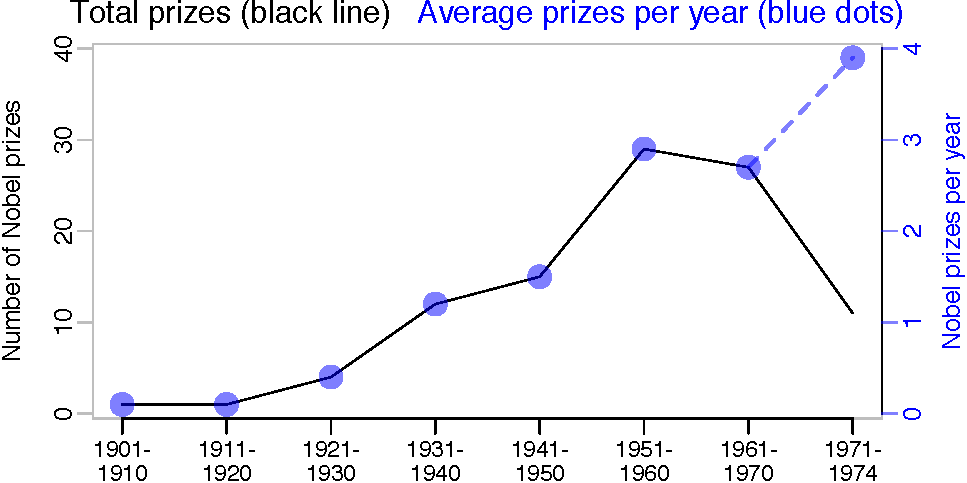
\includegraphics[width=0.8\linewidth]{02-graphs_files/figure-latex/Nobel-1} 

}

\caption{The black line shows numbers of US Nobel prizes, for given time intervals. The gray dots. with the right axis label, show average per year.}\label{fig:Nobel}
\end{figure}

The same principle applies for intervals of measures other than time --- for example of length or volume.

\section{Banking --- the importance of aspect ratio}\label{banking-the-importance-of-aspect-ratio}

\begin{figure}[H]

{\centering 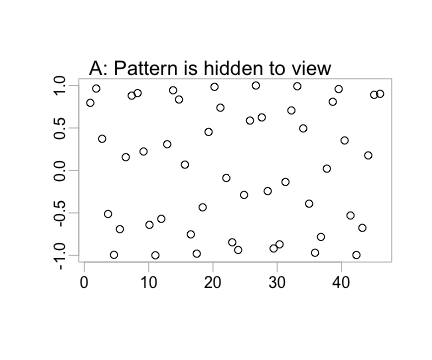
\includegraphics[width=1\linewidth]{02-graphs_files/figure-latex/Banking-1} 

}

\caption{The same data are used for both graphs.  The pattern that is not
obvious in Panel A is very obvious in Panel B}\label{fig:Banking}
\end{figure}

Patterns of change on the horizontal scale that it is important to identify should bank at an angle of roughly 45\textsuperscript{o} above or below the horizontal. Angles in the approximate range 20\textsuperscript{o} to 70\textsuperscript{o} may be satisfactory, and the aspect ratio should be chosen accordingly.

\section{Scales that show changes by equal multipliers}\label{scales-that-show-changes-by-equal-multipliers}

Figure \ref{fig:animals} shows two plots of the same data. Panel A plots brain weight (grams) against body weight (kilograms), for 28 ``animals''. Panel B plots the same data, but now equal distances on each scale show changes by the same factor (i.e., change in relative weight).

\begin{figure}[H]

{\centering 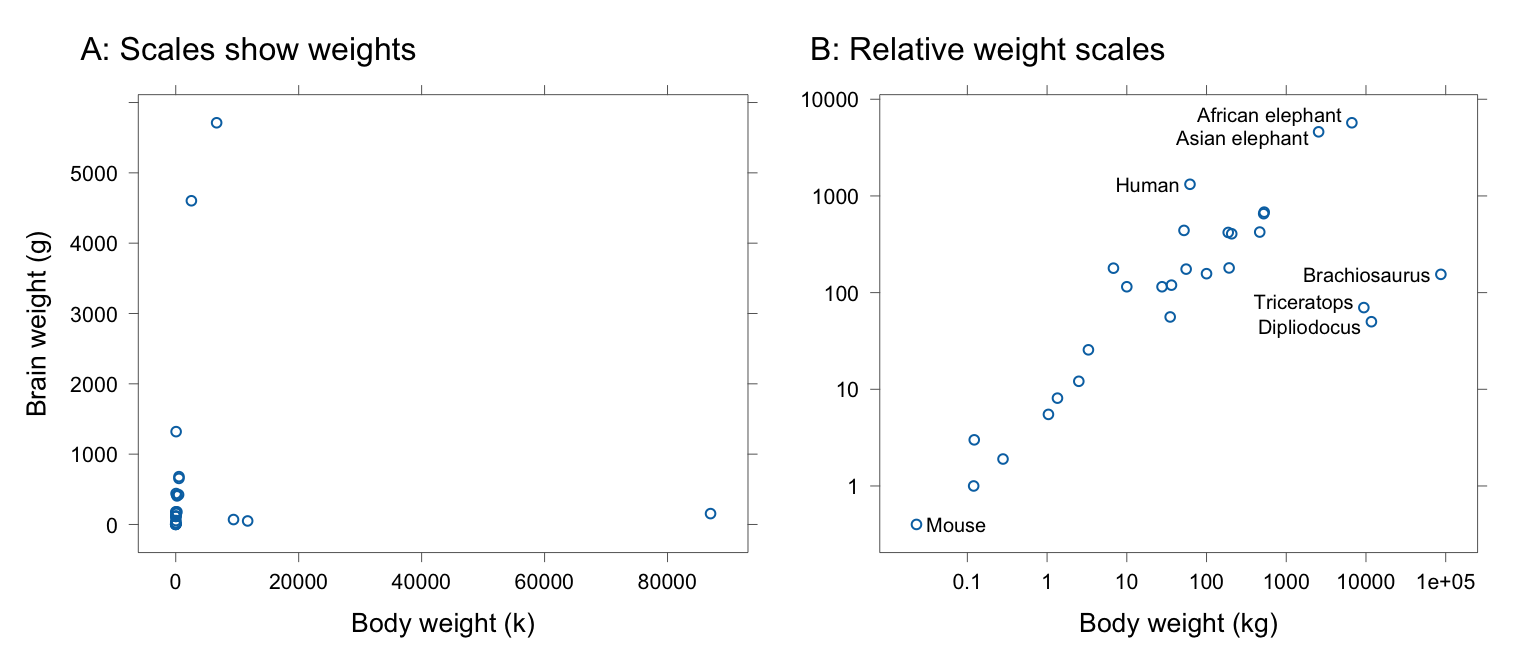
\includegraphics[width=1\linewidth]{02-graphs_files/figure-latex/animals-1} 

}

\caption{Panel A plots brain weight (grams) against body weight 
(kilograms), for 28 'animals'.  Panel B plots the same data, 
with relative weight scales, i.e., equal distances on each scale 
show changes by the same multiplier.}\label{fig:animals}
\end{figure}

Often, when measurement data span a large range (e.g., a change from smallest to largest by a factor of 100 to 1 or more), it is a relative amount scale that is appropriate.\footnote{Technically, such scales are termed logarithmic,~as opposed to straight line or linear. A logarithmic transformation is used to obtain such relative distance scales.}

\section{Different graphs serve different purposes}\label{track}

The line in Figure \ref{fig:resid}A shows the broad overall pattern, while Figure \ref{fig:resid}B shows how that pattern needs to be tweaked to more closely reflect the data.

\begin{figure}[H]

{\centering 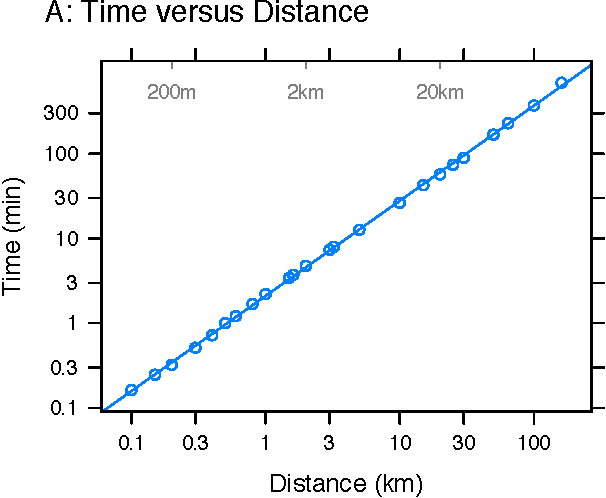
\includegraphics[width=1\linewidth]{02-graphs_files/figure-latex/resid-1} 

}

\caption{Panel A plots world record Time (as of 2006, in minutes)
against Distance (in kilometers), for field races.  On both the
`x` and `y` axes, the scale is one on which equal distances on 
the scale correspond to equal relative changes.  Panel B plots
deviations from the fitted line in the `y` direction, otherwise
known as residuals, against Distance. The deviations are
approximate relative differences from the line.  Thus a 0.05
difference is a difference that amounts to 5\% of the time
predicted by the line.}\label{fig:resid}
\end{figure}

Notice, in Panel A, the use of scales for which which equal distances on the scale correspond to equal relative changes. This is achieved by specifying logarithmic scales, on both axes. There is a loglinear, i.e., straight line on logarithmic scales, relationship.

In Figure \ref{fig:resid}, the line looks to be a good fit. The range of times is however large, from just under 10 seconds to close to 11.5 hours. All except the largest difference from the fitted line are a less than 7\% change, and are not at all obvious in Panel A. There is a very clear pattern of systematic differences in Panel B that reflects differences in human physiology, very likely between the athletes who excel at the different distances.

The line can be interpreting as implying a 13\% increase in the time per unit distance for every unit increase in the distance. The units may for example be units of 100 meters, or kilometers. Panel B indicates that the pattern of increase moves down to a local minimum at around 200 meters, up to a local maximum at around 1 kilometer, down again to a local minimum at around 20 kilometers, and then steadily up again.

\subsection*{Relative distance scales}\label{relative-distance-scales}
\addcontentsline{toc}{subsection}{Relative distance scales}

Figure \ref{fig:lnscales} shows different ``equal physical distance along the scale'' labels that might be used for the relative \texttt{Distance} (``logarithmic'') scale in Figure \ref{fig:resid} in Subsection \ref{track}.

\begin{figure}[H]

{\centering 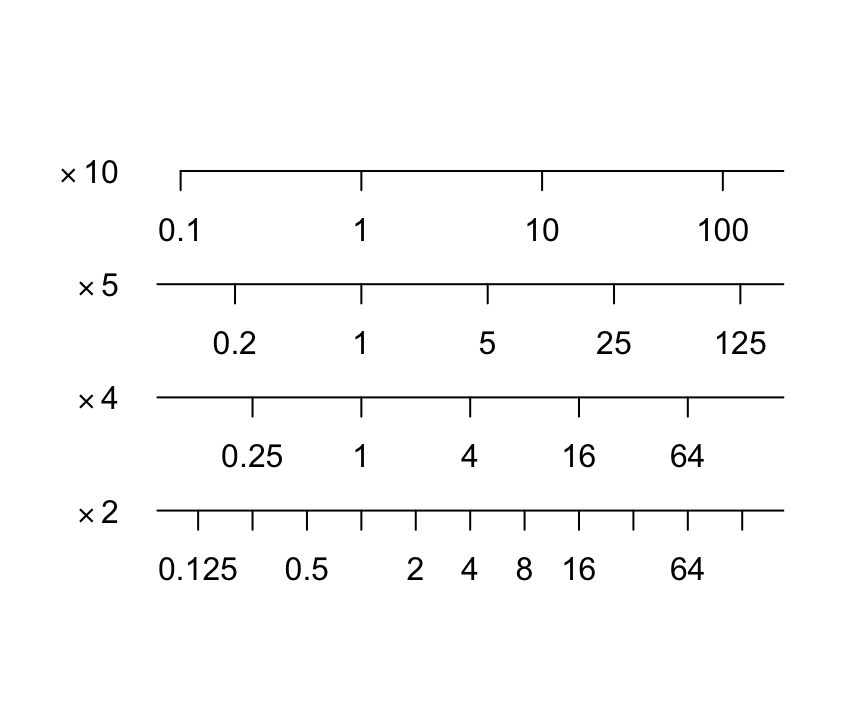
\includegraphics[width=0.6\linewidth]{02-graphs_files/figure-latex/lnscales-1} 

}

\caption{Different labelings, all with tick marks at the same
relative distance apart, are shown for the `Distance` scale.
The multipliers for the `Distance` values that are plotted are,
starting at the bottom, 2, 4, 5, and 10.}\label{fig:lnscales}
\end{figure}

\section{Helpful web links are:}\label{helpful-web-links-are}

\begin{itemize}
\tightlist
\item
  Good \& bad graphs (Ihaka, lecture notes)\footnote{\url{https://www.stat.auckland.ac.nz//~ihaka/120/Lectures/lecture03.pdf}}
\item
  Misleading graphs\footnote{\url{https://www.statisticshowto.com/misleading-graphs/}}
\item
  Color Brewer\footnote{\url{https://colorbrewer2.org/}}
\end{itemize}

\chapter{Selection and survivor bias}\label{selection-and-survivor-bias}

In mind here are cases where the data are not a random sample.

\section{The hazards of convenience samples}\label{the-hazards-of-convenience-samples}

Quota sampling has often been used as an alternative to random
sampling --- quotas are set for age categories, male/female,
and socioeconomic categories that are designed to ensure that
the sample~is representative of the wider population.
In polls~prior to the 1948 US presidential election that
pitted democrat Harry Truman against republican Thomas Dewey,
pollsters were given strict quotas, but otherwise left~free to
decide who they would approach. Polls by three different
organizations gave Dewey a lead of between 5\% and 15\%. In the
event, Truman led by 5\%.

\subsection*{Convenience samples sometimes have a story to tell}\label{convenience-samples-sometimes-have-a-story-to-tell}
\addcontentsline{toc}{subsection}{Convenience samples sometimes have a story to tell}

This is not to rule out all use of convenience samples.
Convenience samples, taken within a limited population,
can sometimes be useful in setting a bound.
It is strongly in the public interest that scientists have
reasonable freedom for responsible expression of their minds
on issues of public concern. In an informal 2015 survey, 151
Crown Research Institute scientists (out of 384 who responded)
answered yes to the question ``Have you ever been prevented
from making a public comment on a controversial issue by your
management's policy, or by fear of losing research funding?''
The 384 who responded will undoubtedly be a biased sample.
Irrespective of the size of the bias, the number who had not
been allowed to speak their mind was large enough to be a cause
for serious concern. Hon Joyce's response, to the effect that
as this was not a scientific survey of all CRI scientists
(to this extent, true), its evidence of large concern could be
ignored, was an evasion. Equally disturbing was the reaction
of the NIWA management, suggesting that they did not accept a
responsibility to defend transparency.\footnote{See \url{https://sciblogs.co.nz/infectious-thoughts/2015/08/28/niwa-in-astonishing-attack-on-scientist-association/}}

\section{UK cotton worker wages in the 1880s}\label{uk-cotton-worker-wages-in-the-1880s}

Prior to the Boot and Maindonald (\citeproc{ref-boot2008new}{2008}) paper\footnote{``New estimates of age- and sex- specific
  earnings and the male-female earnings gap in the British cotton
  industry, 1833-1906''} the main source of published information on
cotton worker wages in the UK in the late 19th century were results
from an 1889 US Bureau of Labor survey, intended for~use for
comparison with the US cotton industry wages.

\begin{figure}

{\centering 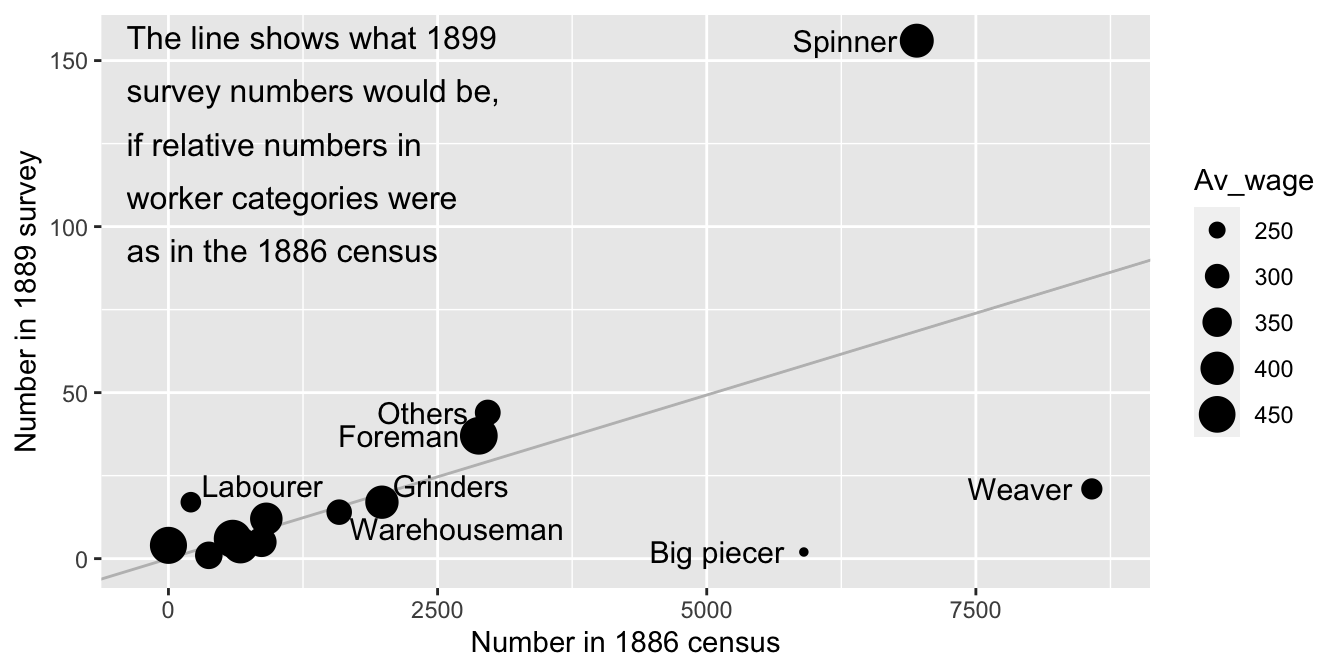
\includegraphics{03-select_files/figure-latex/cotton-1} 

}

\caption{Cotton worker wages in the UK --- 1889 US Bureau of Labor 'survey'
versus 1886 census data. Wages are in pence per week.}\label{fig:cotton}
\end{figure}

Figure \ref{fig:cotton} compares the US Bureau of Labor
survey numbers with 1886 census numbers of different types
of full time UK cotton operatives.
The 1889 survey shows some strong biases --- a result it
would seem of geographical bias and of the informal data
collection methods that were used. The high wages given to
spinners were grossly over-weighted in the US Bureau of
Labor survey, while Big Piecers and Weavers were grossly
under-represented. A guess is that workers were asked for
information on their wages as they left work, and that
the survey personnel happened to catch employees at a time
when there was a large preponderance of highly paid spinners,
and an untypically small number of big piecers and weavers.
The net effect was a gross over-estimate of average wages.

\section{The uneasy path from hindsight to insight}\label{the-uneasy-path-from-hindsight-to-insight}

There is a mix of selection and survivor bias when data
from the past are used as a guide to the future, with no
allowance for the source/target difference. The target about
which we wish to~make judgments lies in the future, while the
data are from the past. Think about a business that is
planning for the future. One can never know, until after the
event, all the ramifications of the choices made.

Businesses may be selected as examples of effective business
practice because they were, at the time when the data were
collated, successful. Likewise, it is athletes who have
been successful in the recent past who are likely to be
selected to~appear on the covers of sports magazines.
In either case, this gives a biased picture of what can be
expected in the future --- in many cases those who are
picked out will be close to~the peak of their success,
and/or have had unusual luck. High levels of success in
the recent past will not always translate into success
in the following year or years. How often will past
success translate into future success? In order to
discover, it is necessary to collect relevant data.

\subsection*{Tales of standout past success}\label{tales-of-standout-past-success}
\addcontentsline{toc}{subsection}{Tales of standout past success}

Collins (\citeproc{ref-collins_2001}{2001}), in the book \emph{Good to Great}, identified
11 companies, from 1,435 studied, as standouts. Since 2001,
5 have performed better than average, and 6 worse.
Notable later changes in fortune were

\begin{itemize}
\tightlist
\item
  Fannie Mae --- 2001: \textgreater\$80 per share: 2008: \textless\$1
\item
  Circuit City: Bankrupt in 2009
\end{itemize}

Waterman and Peters (\citeproc{ref-waterman1982search}{1982}), in the book \emph{Close to consumer''},
identified 43 successful companies, as having a ``bias for action'',
and being ``close to consumer''. From the 35 that were publicly listed,
Smith (\citeproc{ref-smith-sd}{2014}) noted that 15 had done better than average, and 20 worse.
See Smith (\citeproc{ref-smith-sd}{2014}) for further commentary.

In all cases, companies that were chosen as examples of
standout success were likely to be near to~the peak of
their performance, as judged by Collins, or by Waterman and Peters.
Overlaid on this is the regression effect that will be discussed
in Chapter \ref{sec:reg}.

\section{The message in the missing bullet holes}\label{ss:wald}

In World War II, the US air force was concerned that too many
of their planes were being shot down. What were the priority
areas to which protective armour should be added, given that
the extra weight meant that they could not be placed everywhere?
Abraham Wald's insight was that survivor bias was to be
expected, with the density of bullet~holes providing evidence
about the extent of bias, and the implications for identifying
the part(s) of the planes that would benefit most from
additional protection. See \href{https://medium.com/@penguinpress/an-excerpt-from-how-not-to-be-wrong-by-jordan-ellenberg-664e708cfc3d}{Abraham Wald and the Missing Bullet Holes}\footnote{\url{https://medium.com/@penguinpress/an-excerpt-from-how-not-to-be-wrong-by-jordan-ellenberg-664e708cfc3d}},
which is~an excerpt from Ellenberg (\citeproc{ref-ellenberg_2015}{2015}).

The~numbers of hits per square foot were:

\begin{verbatim}
      Engines      Fusilage   Fuel system Rest of plane 
         1.11          1.73          1.55          1.80 
\end{verbatim}

Wald argued that the gunshots were likely to have been spread
very nearly uniformly over the planes as a whole, those that
were shot down, and those that survived, The reason for relatively
fewer bullet holes in the engine and fuel system areas was that
hits in those areas were more likely to bring the plane down,
so~that they did not return.

\chapter{Medicine and health}\label{medicine-and-health}

A focus on medicine and public health is used as a context in which to introduce ideas and issues that are more generally relevant. There is wide acceptance that the evidence provided by randomized controlled trials (RCTs) that are conducted to high standards is at the top of a hierarchy of evidence.

Web sources are noted that, because they base their advice on careful and transparent evaluations of the available evidence, can be trusted.

\section{Useful sources of advice and information}\label{useful-sources-of-advice-and-information}

Here are noted web resources that, for many issues of major interest, provide carefully collated assessments that are based on a critical examination of the whole range of evidence that the authors could identify. There may be many published studies, not all of equal quality, that bear on a medical~issue. Or there may be one, or a small number, of large-scale high quality trials that are used as a basis for judgment. It is important that assessments are updated as new evidence emerges.

Resources that will be noted are

\begin{itemize}
\tightlist
\item
  \href{https://www.hardingcenter.de/en}{Harding Center for Risk Literacy}
\item
  The \href{https://www.cochrane.org/}{Cochrane Center}
\item
  \href{https://wintoncentre.maths.cam.ac.uk/}{Winton Centre for Risk and Evidence Communication}
\end{itemize}

\href{https://medlineplus.gov/}{Note also the US Consumer health information site}

\subsection*{The Harding Center for Risk Literacy}\label{the-harding-center-for-risk-literacy}
\addcontentsline{toc}{subsection}{The Harding Center for Risk Literacy}

There is extensive informative content on the \href{https://www.hardingcenter.de/en}{Harding Center for Risk Literacy site.}\footnote{\url{https://www.hardingcenter.de/en}} Note in particular

\begin{itemize}
\tightlist
\item
  Medical Fact Boxes. Look under \textbf{Transfer and Impact \textbar{} Fact Boxes}
\item
  Covid-19. Look under \textbf{Transfer and Impact \textbar{} Corona pandemic}
\item
  Consumer Empowerment. \textbf{Transfer and Impact \textbar{} Consumer Empowerment}
\item
  Risk and Evidence Communication. Look under \textbf{Research \textbar{} Risk and Evidence Communication}
\item
  VisRisk - Visualization and Communication of Complex Evidence in Risk Assessment. Look under \textbf{Research \textbar{} VisRisk}
\item
  Horizon2020 Project FORECEE (on balancing female cancer risk against the risk arising from false-positive alarms and overdiagnosis). Look under \textbf{Research \textbar{} FORECEE Project}
\item
  Drone Risks Project. Look under \textbf{Research \textbar{} Drone Risks Project}
\item
  Publications. Look under \textbf{The Harding Center \textbar{} Publications}
\item
  In the Media. Look under \textbf{The Harding Center \textbar{} In the Media}
\end{itemize}

\subsection*{Harding Center Medical Fact Boxes}\label{harding-center-medical-fact-boxes}
\addcontentsline{toc}{subsection}{Harding Center Medical Fact Boxes}

\href{https://www.hardingcenter.de/en/transfer-and-impact/fact-boxes}{Medical fact boxes}\footnote{\url{https://www.hardingcenter.de/en/transfer-and-impact/fact-boxes}} provide visual and tabular summaries of the current ``best'' evidence, from randomized controlled trials. The comparison may be with a placebo, or with an alternative that is known to be effective. Detailed references are given. Where available, reliance is on Cochrane studies. Available fact boxes, as of March 2024, appear under the headings:

\begin{itemize}
\tightlist
\item
  Vaccines
\item
  Low back pain
\item
  Antibiotics
\item
  Early detection of cancer: breast, colon, prostate, ovarian
\item
  Cardiovascular Diseases
\item
  Osteoarthritis of the knee
\item
  Tonsil surgery
\item
  Pregnancy and childbirth
\end{itemize}

Scroll down the home page\footnote{\url{https://www.hardingcenter.de/en}} to find the headings \textbf{Risk Literate} (with a link to a risk quiz), and \textbf{Quick Risk Test} (with a link to a test that is targeted at medical students and medical professionals. On the development of this latter test, see Cokely et al. (\citeproc{ref-cokely2012measuring}{2012}).

\subsection*{\texorpdfstring{The Cochrane Center\footnote{\url{https://www.cochrane.org/}}}{The Cochrane Center}}\label{the-cochrane-center04-medical-4}
\addcontentsline{toc}{subsection}{The Cochrane Center}

The Cochrane Center's mission is ``to promote evidence-informed health decision-making by producing high-quality, relevant, accessible systematic reviews and other synthesized research evidence.'' They rely heavily on meta-analyses, looking for the balance of evidence across all relevant studies.

\section{Randomized Controlled Trials vs other study types}\label{ss:rct}

Two types of study are widely used in medical and other contexts --- randomized controlled trials (RCTs), and population-based studies. These can, in both cases, be broken down into further sub-types. There may be elements of both these types of studies.

\subsection*{Randomized Controlled Trials --- the gold standard?}\label{randomized-controlled-trials-the-gold-standard}
\addcontentsline{toc}{subsection}{Randomized Controlled Trials --- the gold standard?}

For simplicity, it will be assumed that there are two alternatives to be compared, in what is known as a two-armed trial. In medical trials the two arms may be a treatment and a placebo, with the placebo (something harmless that has no effect) made to look as similar as possible to the treatment.

An important distinction is between pre-clinical trials, often with animals such as mice, and clinical trials with human subjects. Pre-clinical trials are likely to be conducted with a small number of mice or other animals, and are intended to check whether a drug or other treatment warrants further investigation. Evidence will be presented in Section \ref{sec:lab} that suggests that these trials are commonly not achieving their intended purpose.

Clinical trials typically are conducted in three phases. Phase I applies the treatment to a small number of subjects and checks that the treatment appears safe. Phase II, perhaps with several hundred subjects, looks for evidence of an effect, and how this might relate to dose level. Phase III trials are conducted with large numbers of subjects, typically spread over multiple treatment centres, and are designed to check whether the treatment is effective, what side effects there may be, and whether there are issues with particular subgroups.

Important issues are

\begin{itemize}
\tightlist
\item
  Use a random mechanism to assign to assign to treatment as against control --- in a medical screening study to ``screen'' or ``not screen''

  \begin{itemize}
  \tightlist
  \item
    The aim is to ensure that apples are compared with apples
  \item
    Treatment and control must otherwise be treated in the same way.
  \end{itemize}
\item
  There must be strict adherence to a protocol

  \begin{itemize}
  \tightlist
  \item
    Minor departures that may, e.g., allow unconscious bias in the way that results from the different groups of participants are measured, can invalidate results.
  \item
    In clinical trials an ideal, not always possible, is the double blind trial where neither the individual nor the clinician involved knows which drug (or other treatment) the individual has received.
  \end{itemize}
\item
  Results apply, strictly, to those who meet the trial entry criteria

  \begin{itemize}
  \tightlist
  \item
    This may limit relevance to the general population
  \end{itemize}
\end{itemize}

Especially in medical trials, think carefully about the outcome measure. It is not enough to show that a screening program will pick up otherwise undiagnosed cancers.

\begin{itemize}
\tightlist
\item
  In a screening trial, e.g., for prostate cancer, there are risks both for those who test positive, and for those who test negative.

  \begin{itemize}
  \tightlist
  \item
    The process used to check for cancer may itself bring a smaller or larger element of risk.
  \item
    Positives may be false positives, leading to more invasive checks which~may themselves carry a risk. Thus, for prostate cancer, a positive PSA test is likely to lead to a biopsy that itself has been estimated to carry a 5\% risk of serious side effects, with a much higher proportion of less serious effects (\citeproc{ref-levitin_2015}{Levitin 2015, 245})
  \item
    Some slow growing cancers may be better left untreated, rather than exposing the patient to a treatment that may itself do serious damage.
  \end{itemize}
\end{itemize}

For a helpful animated summary of some of the key issues, see:\\
\url{https://www.youtube.com/watch?v=Wy7qpJeozec}. Pashayan et al. (\citeproc{ref-pashayan2020personalized}{2020}) provide an overview of progress towards the personalized early detection and prevention of breast cancer, noting priority areas for action.

\subsection*{A note in passing: HiPPO decisions vs A/B testing}\label{a-note-in-passing-hippo-decisions-vs-ab-testing}
\addcontentsline{toc}{subsection}{A note in passing: HiPPO decisions vs A/B testing}

Randomized studies are widely used outside of medicine. Randomization is a key component of the way that Google and others test out, e.g., the effect of different web page layouts.

\begin{itemize}
\tightlist
\item
  HiPPO = ``Highest paid person in the Office.''
\item
  The term ``A/B testing'' is sometimes used to refer to randomized testing of alternatives.
\end{itemize}

A/B testing helped propel Obama into office! An experiment was conducted that involved 15 million people, or~about 25\%, from its email list. The signup forms had one of nine different combinations of images with words on which recipients were invited to click, thus:

\begin{tabular}{lccc}
& Learn more & Join us & Sign up now \\
Obama photo & \ding{56} & \ding{56} & \ding{56} \\
BW photo of Obama family & \ding{52} & \ding{56} & \ding{56} \\
Obama speaking & \ding{56} & \ding{56} & \ding{56} \\
\end{tabular}

The black and white photo of the Obama family, with the words ``Learn more'', generated the most clicks.

Young (\citeproc{ref-young2014improving}{2014}) gives an account of A/B testing as it might be used for improving library user experience.

\subsection*{Population studies --- groups must be broadly comparable}\label{population-studies-groups-must-be-broadly-comparable}
\addcontentsline{toc}{subsection}{Population studies --- groups must be broadly comparable}

\begin{itemize}
\tightlist
\item
  Adjust prunes to look like apples (is it possible?)
\item
  Can one ever be sure that the adjustments do the job?
\item
  Potential for biases is greater than for randomized controlled trials.
\end{itemize}

Where a treatment is compared with a control group, the idea is to use a regression type approach to adjust for differences in such variables or factors as age, sex, socioeconomic status, and co-morbidities. ``Propensity score'' approaches try to summarize such group differences in a single variable (or, in principle, two or more variables) that measure the propensity to~belong to the treatment as opposed to the control group. While their effectiveness for this purpose may be doubted, they can be used to provide insightful graphs that check the extent to which the groups are broadly comparable on the variables and/or factors used to adjust for differences.

The generally negative view of observational studies that is presented in Soni et al. (\citeproc{ref-soni2019comparison}{2019}) (studies in oncology) contrasts with the more positive view offered in Anglemyer, Horvath, and Bero (\citeproc{ref-anglemyer2014healthcare}{2014}) (health care), for observational studies that have been conducted with high methodological rigour. The strongest evidence comes, as with the link between smoking and lung cancer, from multiple studies, with different likely biases, that all point strongly in the same direction.

\subsection*{Issues for all types of study}\label{issues-for-all-types-of-study}
\addcontentsline{toc}{subsection}{Issues for all types of study}

What are the relevant outcome measures?

\begin{itemize}
\tightlist
\item
  e.g., cancer -- malignancies found \& removed, or deaths

  \begin{itemize}
  \tightlist
  \item
    deaths from cancer, or from all causes (for some individuals, the treatment may be more damaging in it medium to long term effect than the cancer)
  \end{itemize}
\end{itemize}

Care is required to deal with survivor, as well as other, biases.

\subsection{False Positives}\label{false-positives}

In contexts where the number of false positives is likely to be high relative to the number of true positives, screening programs may have serious downsides that outweigh the benefits.

Excess iron syndrome, known as ``haemochromatosis'', affects around 1 in 200 in the New Zealand population. Consider a test that has an 80\% accuracy, both for detecting the syndrome among those who have it, and for not detecting among those who do not.\footnote{These are known as the ``sensitivity'', and the ``specificity''.}

Excess iron syndrome, known as ``haemochromatosis'', affects around 1 in 200 in the New Zealand population. Consider a test that has an 80\% accuracy, both for detecting the syndrome among those who have it, and for not detecting among those who do not.\footnote{These are known as the ``sensitivity'' (true positive~rate''), and the ``specificity'' (true negative rate).}\\
Among 2000 tested (10 with and 1990 without)

\begin{itemize}
\tightlist
\item
  there will on average be \textbf{8} out of 10~true positives
\item
  the 1990 without the syndrome will split up~as detected +ve to detected -ve in an 20\%:80\% ratio. Thus there will be, on average, .2 \(\times\) 1990 = \textbf{398} false positives.
\end{itemize}

Overall, those detected as positive split up in a true:false ratio of 8:398, i.e., 8/406 or just under 2\% of the positives are false positives. If all positives were detected as positive, the 8/406 would change to 10/406.

A test with this kind of accuracy becomes much more useful in a subset of the population already known to be at high risk, perhaps as identified by a genetic test, or perhaps because of a medical condition commonly associated with the syndrome.

\section{Hierarchies of evidence}\label{hierarchies-of-evidence}

There is broad agreement among medical researchers on the hierarchy of evidence that is set down in the (\citeproc{ref-us1989guide}{US Preventive Services Task Force 1989}) guide:

\begin{itemize}
\tightlist
\item
  Level I: Evidence obtained from at least one properly designed randomized controlled trial.
\item
  Level II-1: Evidence obtained from well-designed controlled trials without randomization.
\item
  Level II-2: Evidence obtained from well-designed cohort studies or case-control studies, preferably from more than one centre or research group.
\item
  Level II-3: Evidence obtained from multiple time series designs with or without the intervention. Dramatic results in uncontrolled trials might also be regarded as this type of evidence.
\item
  Level III: Opinions of respected authorities, based on clinical experience, descriptive studies, or reports of expert committees.
\end{itemize}

The CONSORT 2010 statement (\citeproc{ref-Schulzc332}{Schulz, Altman, and Moher 2010}) sets out detailed criteria for assessing randomized controlled trials (RCTs). For Level II studies, the STROBE guidelines (\citeproc{ref-erik2007strengthening}{Erik von Elm et al. 2007}) set out reporting standards.

Use of such criteria is essential when evidence that is available from multiple randomized controlled trials, perhaps supplemented by evidence from studies at lower levels of the hierarchy, is brought together in a systematic review. Evidence at level II, and especially at level II-3, should ideally be checked by conducting an RCT. This is not always possible, for ethical or practical reasons.

Evidence from one type of study may complement evidence from another. A paper entitled ``Resolved: there is sufficient scientific evidence that decreasing sugar-sweetened beverage consumption will reduce the prevalence of obesity and obesity-related diseases'' (\citeproc{ref-hu2013resolved}{Hu 2013}) provides an example. Hu brings evidence from short-term randomized controlled trials together with evidence from long term cohort studies (4 or 8 years) to make a convincing case.

Clinical trials have their own problems and issues. Using evidence from published review sources, Chalmers and Glasziou (\citeproc{ref-chalmers2009avoidable}{2009}) found issues with the choice of research questions; the quality of research design and methods, and the adequacy of publication practices. They reported that 50\% of studies were designed without reference to systematic reviews of existing evidence, and that 50\% were~never published in full.

Planning and execution failures are set in stone by the time that a research report is sent for review. Pre-registration, involving the depositing a research question and study design with a registration service or journal before starting an investigation, allows peer review feedback that can elicit suggestions for improvement and detect any potential flaws before the study begins.\footnote{See \url{https://plos.org/open-science/preregistration/}} Even more than for industrial~quality control,~processes are needed that prevent defects from appearing in the first place, with screening for defects at the end of the production line used as a check that those processes have done the job asked of them.

Chapter \ref{ch:obs} will discuss issues for using observational data as a basis for inferences.

\section{Avoid, or expose infants~to~peanuts?}\label{avoid-or-expose-infants-to-peanuts}

Clinical practice guidelines introduced in or around the year 2000 had ``recommended the exclusion of allergenic foods from the diets of infants at high risk for allergy, and from the diets of their mothers during pregnancy and lactation.''

It was then a surprise to find that the prevalence of peanut allergy has substantially increased in the recent past, doubling in Europe between 2005 and 2015, suggesting that advice given to parents of young children to avoid foods containing peanuts may have been counterproductive. This reassessment was supported, at least for infants who at four months had either severe eczema or food allergy or both, and thus were at high risk of developing a peanut allergy, by the LEAPS study reported in Du Toit et al. (\citeproc{ref-du2015randomized}{2015}).

As noted, the LEAPS study was limited to infants who at four months had either severe eczema or food allergy or both. Infants were stratified into two groups following a skin-prick test, with each group then randomized between those exposed to peanut extract, and those not exposed.

Among 530 infants in the population who initially had negative results on the skin-prick test, the prevalence of peanut allergy at 60 months of age was 13.7\% (37/270) in the avoidance group and 1.8\% (5/272) in the consumption group.\footnote{There were twelve further infants in this group~whose results could not be evaluated.} Among the 98 participants who initially had positive test results, the prevalence of peanut allergy was 35.3\% (18/51) in the avoidance group and 10.6\% (5/47) in the consumption group. There was no between-group difference of consequence in the incidence of serious adverse events.

In both groups, numbers and percentages are for those who were assigned to the group and whose results could be evaluated, whether or not they followed the treatment protocol to which they were assigned. In technical terms, these are results from an ``intention to treat'' analysis. Such an analysis is designed to mirror what can be expected in practice --- not everyone who starts off in one group will stick to~it. It answers questions about what to do with subjects who did~not fully follow the treatment to which they were assigned.

The results were followed, in 2016, by changes to guidelines that recommended introduction of peanut and other allergenic foods before 12 months. The assumption that avoiding early exposure to peanuts would reduce risk of later development of peanut allergy was, it was judged, likely wrong for all~infants.

\section{The effectiveness of surgery -- RCTs are challenging}\label{the-effectiveness-of-surgery-rcts-are-challenging}

The blurb on the back cover of Harris (\citeproc{ref-harris2016book}{2016}) states that

\begin{quote}
For many complaints~and conditions, the benefits from surgery are lower, and the risks higher, than you or your surgeon think.
\end{quote}

Humans are very prone to the \emph{post hoc, ergo propter~hoc} fallacy: ``it followed, therefore it was because of'' fallacy. Harris argues that unless the benefits of a surgical procedure are clear, the only ethical way forward is to do a randomized trial where the procedure is compared with a sham procedure. Such trials are not easy to design and execute. Nonetheless, there are a number of important cases where such comparisons have been made.

Bloodletting is a prime example of a surgical procedure that has faded away due to evidence,~not just of a lack of effectiveness,~but of serious harm.\footnote{For the history, see for example Seigworth (\citeproc{ref-seigworth1980bloodletting}{1980})} The practice attracted widespread debate in the 19th century and into the early 20th century, with its defenders making such claims as

\begin{quote}
``blood-letting is a remedy which, when judiciously employed, it is hardly possible to estimate too highly''
\end{quote}

A comment in Watkins (\citeproc{ref-watkins2000conviction}{2000}) is apt

\begin{quote}
Medical evidence is trusted, and we must retain that situation and ensure that it is not abused. It is possible to be an extremely good doctor without being numerate, and not every eminent clinician is best placed to give epidemiological evidence. Doctors should not use techniques before they have acquainted themselves with the principles underlying them.
\end{quote}

What are the implications for medical practice?

\section{Screening for cancer --- how relevant is historical evidence}\label{screening-for-cancer-how-relevant-is-historical-evidence}

Screening for cancer is an area where, if the interest is in risk of death, it is necessary to wait for perhaps several decades before there is a high enough number of deaths that results can be usefully evaluated. Changes that can be expected in the interim include:

\begin{itemize}
\tightlist
\item
  Screening may become more sensitive, perhaps picking up a higher proportion of relatively benign cancers that are unlikely to ever have serious effects.\\
\item
  There may be an increased ability to distinguish between benign and more aggressive cancers.\\
\item
  More effective and/or less invasive treatments may become available, and earlier treatments finessed.
\end{itemize}

All cause death rates are a more relevant measure than cancer specific death rates, as treatments may themselves have harmful effects. Whether or not results from clinical trials in past decades remain relevant to current circumstances, their results do highlight important questions.

\subsection*{PSA Screening for Prostate Cancer, \& more}\label{psa-screening-for-prostate-cancer-more}
\addcontentsline{toc}{subsection}{PSA Screening for Prostate Cancer, \& more}

Numbers (rounded) in the following table are from a Harding Center fact box. They are for men 50 years or older who either did or did not participate in prostate cancer screening, using the PSA test, for 16 years.\footnote{\url{https://www.hardingcenter.de/en/early-detection-of-cancer/early-detection-of-prostate-cancer-with-psa-testing}}

\begin{longtable}[]{@{}
  >{\raggedright\arraybackslash}p{(\columnwidth - 4\tabcolsep) * \real{0.3662}}
  >{\raggedright\arraybackslash}p{(\columnwidth - 4\tabcolsep) * \real{0.3380}}
  >{\raggedright\arraybackslash}p{(\columnwidth - 4\tabcolsep) * \real{0.2958}}@{}}
\toprule\noalign{}
\begin{minipage}[b]{\linewidth}\raggedright
\end{minipage} & \begin{minipage}[b]{\linewidth}\raggedright
1000 men, No screening
\end{minipage} & \begin{minipage}[b]{\linewidth}\raggedright
1000 men, Screening
\end{minipage} \\
\midrule\noalign{}
\endhead
\bottomrule\noalign{}
\endlastfoot
Deaths (prostate cancer) & 12 & 10 \\
--- & --- & --- \\
Biopsy \& false alarm & 0 & 155 \\
Unnecessary treatment & 0 & 51 \\
\end{longtable}

About 10 out of every 1,000 men with screening, and 12 out of every 1,000 men without screening, died from prostate cancer within 16 years. This means that 2 out of every 1,000 people could be saved from death from prostate cancer by early detection using PSA testing. Deaths from any cause were around 322 in both groups.

Numbers for benefits are based on four studies with about 77,000 participants (progressive cancer), four studies with about 472,000 participants (overall mortality), and eleven studies with about 619,000 participants (prostate cancer specific mortality). The numbers for harms are based on seven studies with approximately 128,000 participants (false-positive results within three to six participations in PSA testing for early detection) and nine studies with approximately 274,000 participants (over-diagnosis and over-treatment). See the web site for references to the studies.

Unlike the biopsies that may follow a positive PSA test, the PSA test has no direct potential to cause physical harm. Harm results from an undue readiness to use the test result as a reason for further potentially harmful testing and treatment. ``Wait and watch'' is often the preferred strategy.

See Martin et al. (\citeproc{ref-martin2018effect}{2018}), Levitin (\citeproc{ref-levitin_2015}{2015}) \[ch. 6\], Fung (\citeproc{ref-fung2020cancer}{2020, 278--81}), the web page \href{https://www.nytimes.com/2011/10/09/books/review/your-medical-mind-by-jerome-groopman-and-pamela-hartzband-book-review.html}{How Patients Think, and How They Should}\footnote{\url{https://www.nytimes.com/2011/10/09/books/review/your-medical-mind-by-jerome-groopman-and-pamela-hartzband-book-review.html}}, and regularly updated summary of the evidence can be found at \href{https://www.ncbi.nlm.nih.gov/books/NBK65906/}{PDQ Cancer Information Summaries}.

\subsection*{Breast cancer screening}\label{breast-cancer-screening}
\addcontentsline{toc}{subsection}{Breast cancer screening}

The Raichand et al. (\citeproc{ref-raichand2017conclusions}{2017}) review starts with the comment:

\begin{quote}
The recent controversy about using mammography to screen for breast cancer based on randomized controlled trials over 3 decades in Western countries has not only eclipsed the paradigm of evidence-based medicine, but also puts health decision-makers in countries where breast cancer screening is still being considered in a dilemma to adopt or abandon such a well-established screening modality.
\end{quote}

The short summary, last updated in October 2019, from the \href{https://www.hardingcenter.de/en/early-detection-breast-cancer-mammography-screening}{Harding Center Fact Box for Mammography Screening}, referring to women 50~years (a few trials looked at women aged \$\geq\$40) and older who either did or did not participate in mammography screening for approximately 11 years reads

\begin{quote}
Mammography reduced the number of women who died from breast cancer by 1 out of every 1000 women. It had no~effect on the number of women who died from any type of cancer. Among all women taking part in screening, some women with non-progressive cancer were over-diagnosed and received unnecessary treatment.\footnote{\url{https://www.hardingcenter.de/en/early-detection-breast-cancer-mammography-screening}}
\end{quote}

The chief English source of evidence for the fact box is the Cochrane review Gøtzsche and Jørgensen (\citeproc{ref-gotzsche2013screening}{2013}). The eight eligible trials included more than 600,000 women aged between 39 and 74, all reported between 1963 and 1991. One trial was excluded because the randomization had not produced comparable groups. Four trials had inadequate randomization. The three trials with adequate randomization did not find an effect of screening on total cancer mortality.

Løberg et al. (\citeproc{ref-loberg2015benefits}{2015}) provide a slightly more detailed breakdown of the evidence, as applied to women who were screened for 20 years, starting at age 50, with mortality assessed at ages 56 to 75 in the UK. Figure \ref{fig:c-screen} is a visual summary. Interval cancers are cancers that are detected in between regular screens. A prior normal screen may give a false assurance and lead to a delay in seeking help when symptoms appear. See also the regularly updated summary of the evidence at\href{https://www.ncbi.nlm.nih.gov/books/NBK65906/}{PDQ Cancer Information Summaries}.

\begin{figure}[H]

{\centering 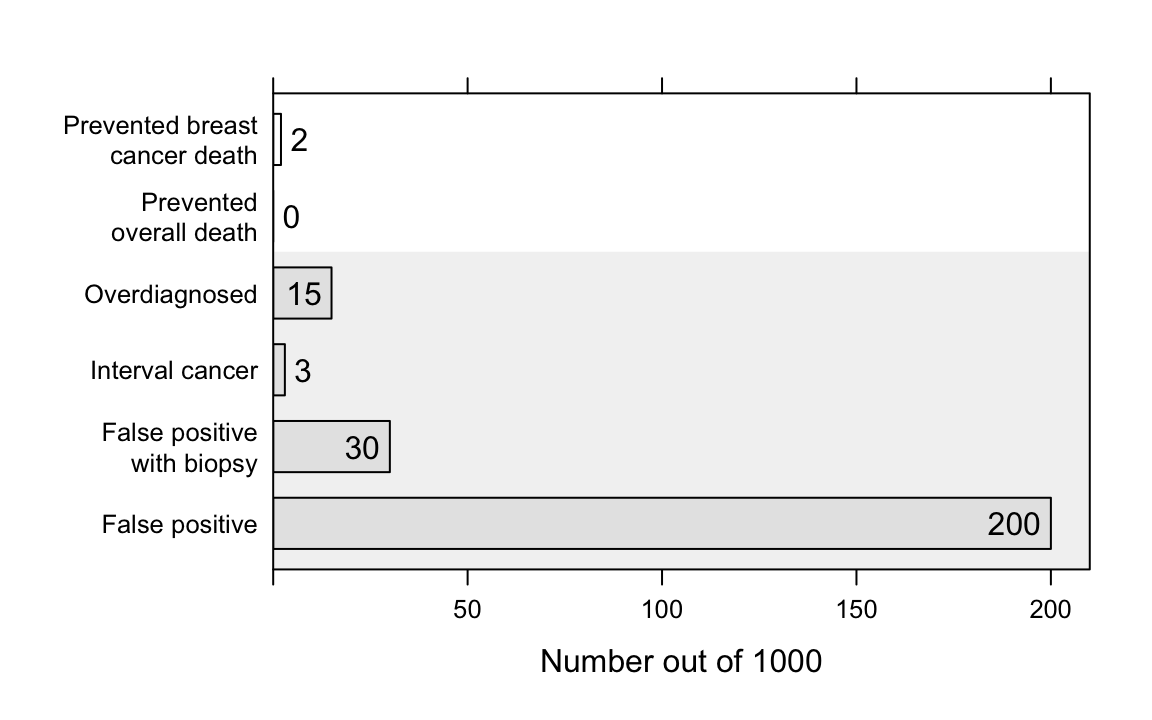
\includegraphics[width=0.6\linewidth]{04-medical_files/figure-latex/c-screen-1} 

}

\caption{Estimates of benefits and harms of screening, as applied to the observed incidence of invasive breast cancer (women aged 50 to 69 years) and mortality (women aged 55 to 74 years) in the UK in 2007.}\label{fig:c-screen}
\end{figure}

The area by area phasing of the introduction of a mammography screening program in Ireland over 1994-2011 had the character of a natural experiment, allowing checks on what the before/after difference of each area as it was phased in, as against areas where the rollout occurred earlier or later. Moran and Cullinan (\citeproc{ref-MORAN2022115073}{2022}) looked at data on the ten-year follow-up of 33,722 breast cancer cases. The conclusion was that ``while invitation to screening increased detection, it did not significantly decrease the average risk of dying from breast cancer in the population.'' The authors did however note that ``screening may have helped to reduce socioeconomic disparities in late stage breast cancer incidence.''

The historical data does, irrespective of questions regarding its current direct relevance, emphasize the importance of tuning breast cancer checks to the risk profile, of finding ways to distinguish progressive from non-progressive cancer, and of avoiding over-treatment. Early diagnosis may allow the use of less invasive forms of treatment. As argued in Esserman and WISDOM Study and Athena Investigators (\citeproc{ref-essermanwisdom}{2017}), women want ``better, not more screening''.

\chapter{The uses and limits of observational data}\label{ch:obs}

At least in principle, it is relatively straightforward to use regression type methods to make predictions for a set of new data that have been sampled in the same way. What is hard for observational data, harder than is commonly acknowledged, is to give the model~coefficients a causal interpretation. For this, it is necessary to have a clear understanding of the processes involved.

\begin{itemize}
\tightlist
\item
  There will be several, perhaps a very large number, of explanatory variables, and an outcome variable.
\item
  The aim is to find a model that will make predictions for new data.
\item
  Note the predictive/descriptive distinction.\\
\item
  Note the ``in sample/out of sample'' distinction.

  \begin{itemize}
  \tightlist
  \item
    But is the ``new'' a random sample of the old population?\\
    (Is the `target' a random sample of the `source'?)
  \end{itemize}
\end{itemize}

\section{We have a prediction. What are the drivers?}\label{we-have-a-prediction.-what-are-the-drivers}

The issues that arise for observational studies do not in general have clear and easy answers. Chapters 20 and 21 of Gelman, Hill, and Vehtari (\citeproc{ref-gelman2020regression}{2020}) canvass points that authors of those studies need to address. See also \href{https://statmodeling.stat.columbia.edu/2018/11/10/matching-discarding-non-matches-deal-lack-complete-overlap-regression-adjust-imbalance-treatment-control-groups/}{Andrew Gelman's blog.}\footnote{\url{https://statmodeling.stat.columbia.edu/2018/11/10/matching-}} There are no simple answers!\footnote{See also \url{https://mathbabe.org/2011/06/16/the-basics-of-quantitative-modeling/}}. All relevant explanatory variables have to be identified, with the manner in which they may be driving predictions then teased out.

Thus, in a comparison between two groups (e..g., in Section \ref{sec:maternity}, midwife led versus medical led neonatal care) one variable or factor may be of particular interest, while other variables are used to adjust for differences between the two groups that are at most a secondary focus of interest. Variables that are of secondary interest are commonly referred to as covariates. Regression coefficients can be misleading guides to what is driving predictions if one or more of the relevant covariates is not available or is not properly accounted for. A paradox of the Yule-Simpson type, sometimes referred to as Laird's paradox, has the same potential to mislead.

Little that has been published since Rosenbaum (\citeproc{ref-RosBook}{2002}) clarifies greatly the advice that can be given for practical data analysis, beyond what Rosenbaum has to say. Pearl and Mackenzie (\citeproc{ref-pearl2018book}{2018}) (``The Book of Why'') offers an interesting assessment. Pearl and his co-author do a good job of highlighting important issues that should be addressed in order to make causality judgments, at the same time overplaying what their methodology can in general achieve. If strictly implemented, the standards are so high that they severely limit what they can in practice achieve. Causality diagrams have a central role. There is a detailed, and insightful, discussion of the history that finally led to the conclusion that smoking causes lung cancer.

\section{Maternal~obesity, and risk of colorectal cancer}\label{maternal-obesity-and-risk-of-colorectal-cancer}

Results from a study reported in Murphy et al. (\citeproc{ref-Murphygutjnl-2021-325001}{2021}) suggest that maternal obesity (≥30 kg/m2) did increase the risk of colorectal cancer (CRC), by a factor of 2.51.\footnote{95\% error bounds, as they are termed, run from 1.05 to 6.02, so that the 2.51 risk factor is not very clearly distinguished from 1.} The authors argue that ``in utero events are important risk factors for CRC and may contribute to increasing incidence rates in younger adults''. They are at the same time careful to acknowledge that, as an observational study, it could not establish cause, and that factors such as diet and microbiome might explain the association. The eating habits of mothers must surely have a large effect on what children eat, both when young and later in life. To what extent might this explain the association.

Obesity is a risk factor for a variety of diseases. Is it obesity that is directly the risk? Or is it dietary and other factors that both increase the risk of obesity and of associated diseases?

\section{Cholera deaths in London --- 1832 to 1855}\label{cholera-deaths-in-london-1832-to-1855}

6,500 died from cholera in London in 1832. Medical opinion blamed ``miasma'' or noxious air, associated with the stink from rotting garbage, faeces, and pollution in the Thames. Poor areas had higher rates of cholera, thought to be a result of the more noxious air that arose from crowding and poorer sanitation. Human excreta went into cesspits, with night-soil periodically taken away.\footnote{See \emph{Cholera epidemics in Victorian London}\newline \url{https://www.thegazette.co.uk/all-notices/content/100519}} In 1842, \href{https://www.sciencemuseum.org.uk/objects-and-stories/medicine/cholera-victorian-london}{Edwin Chadwick, in The Sanitary Conditions of the Labouring Population (1842)}\footnote{\url{https://www.sciencemuseum.org.uk/objects-and-stories/medicine/cholera-victorian-london}} showed a direct link between poor living conditions, disease and life expectancy.

Under the assumption that miasma from the cesspools and raw sewage pits was the source of infection, the 1848 Nuisances Removal and Diseases Prevention Act\footnote{Gazette issue 20637} was passed that led to the dumping of the raw sewage into the Thames, which was London's main source of drinking water. The 1848-49 epidemic followed shortly after the cesspits were banned. Hassall (\citeproc{ref-hassall1850memoir}{1850}), in a careful microbiological study, commented:

\begin{quote}
\ldots{} a portion of the inhabitants are made to consume \ldots{} a portion of their own excrement, and \ldots{} to pay for the privilege.
\end{quote}

\subsection*{By air, or by water --- the 1849 epidemic}\label{by-air-or-by-water-the-1849-epidemic}
\addcontentsline{toc}{subsection}{By air, or by water --- the 1849 epidemic}

Farr, who worked as statistician in the UK Registrar General's~ office, collected data on deaths from cholera in London in the 1849 epidemic. Farr classified districts into three groups thus,\\
according to the source of the water for most of the householders:

\begin{enumerate}
\def\labelenumi{\arabic{enumi})}
\tightlist
\item
  Lower Thames, coded as \texttt{Battersea};\\
\item
  Sources away from the Thames, coded as \texttt{NewRiver};\\
\item
  Further up the Thames than \texttt{Batersea}, where the water was less polluted, coded as \texttt{Kew}.
\end{enumerate}

Figure \ref{fig:Farr} summarizes results from a regression analysis that used Farr's data. None of the terms stands out as substantially more important than any other. Higher rates for the poor, where crowded conditions would commonly make it difficult to maintain hygiene, were to be expected.

\begin{figure}

{\centering 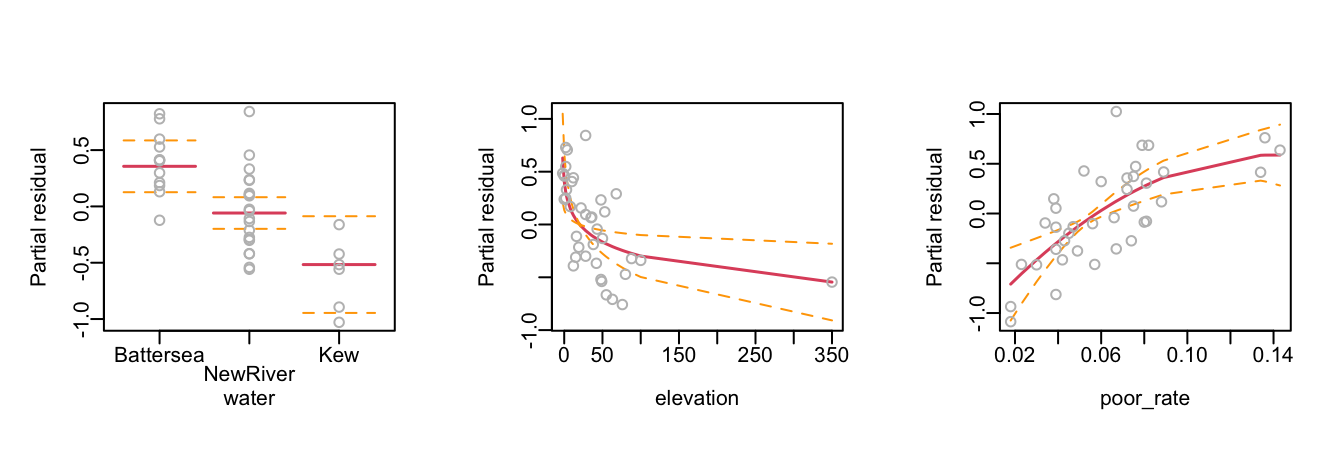
\includegraphics[width=1\linewidth]{05-observational_files/figure-latex/Farr-1} 

}

\caption{Each panel shows, in turn, the estimated contribution
of a term in the model relative to the mean contribution from 
other model terms. Changes in deaths are on a `log` scale, so 
that an increase by one unit multiplies the odds of death by 
close to 2.7, around an overall mean of just over six per 1000.
}\label{fig:Farr}
\end{figure}

Snow (\citeproc{ref-snow1849mode}{1855a}) gave examples that he had observed directly, where the likely means of transmission of the infection appeared to be a water source, or poor hygiene. He argued that those living close to the Thames, and especially in the South, were more likely to be getting their water that was contaminated with human excreta. Contaminants had more time to settle in water that was piped up to higher ground.

Farr took Snow's arguments seriously, but in his 1852 report argued that water was primarily important as a vehicle for miasmata. He would later, by the time of an 1866 epidemic when Snow was dead, be one of the waterborne theory's few champions.\footnote{Eyler (\citeproc{ref-eyler1973william}{1973})}

A context has to be provided in which to~interpret regression results such as those shown in Figure \ref{fig:Farr}. Snow's understanding of the contextual information was not, in 1852, sufficiently compelling to persuade other medical specialists. Data from the 1854 epidemic, which allowed a comparison of deaths supplied from a company that continued to get its supply from lower highly polluted Thames water with that from the company that had moved its supply higher up to less polluted water, seems in retrospect to~clinch the issue, but did not at the time convince most of the medical profession.\footnote{See Eyler (\citeproc{ref-eyler2004changing}{2004}) for further comment.} The perspective brought by germ theory had to wait for the work of Pasteur in the late 1850s and Koch in the 1880s.

\subsection*{The 1854 epidemic --- a natural experiment}\label{the-1854-epidemic-a-natural-experiment}
\addcontentsline{toc}{subsection}{The 1854 epidemic --- a natural experiment}

Two water companies --- Lambeth, and Southwark and Vauxhall, had been taking water from the same polluted source. An 1852 act required water supply companies to move water intake upriver by 1855. By the time of the 1854 epidemic, Lambeth had moved its intake 22 miles upriver,~while the Southwark and Vauxhall intake was unchanged until 1855. Data on the distribution of cholera in the 1854 epidemic then allowed Snow to test the claims made in his 1849 study.

\scalebox{1.12}{
\begin{tabular}{lrrr}
  \hline
 & \#Houses & \#Deaths & Rate per 10,000 \\ 
  \hline
Southwark \& Vauxhall & 40046 & 1263 & 315 \\ 
  Lambeth & 26107 & 98 & 37 \\ 
  Rest of London & 256423 & 1422 & 59 \\ 
   \hline
\end{tabular}
}

\begin{quote}
The experiment, too, was on the grandest scale. No fewer than 300,000 people \ldots, from gentlefolks down to the very poor, were divided into two groups without their choice, and, in most cases, without their knowledge; one group being supplied with water containing the sewage of London, and, amongst it, whatever might have come from the cholera patients, the other group having water quite free from such impurity. (\citeproc{ref-snow1855mode}{Snow 1855b})
\end{quote}

\subsection*{Use water from the brewery, and stay healthy!}\label{use-water-from-the-brewery-and-stay-healthy}
\addcontentsline{toc}{subsection}{Use water from the brewery, and stay healthy!}

\begin{figure}[H]

{\centering 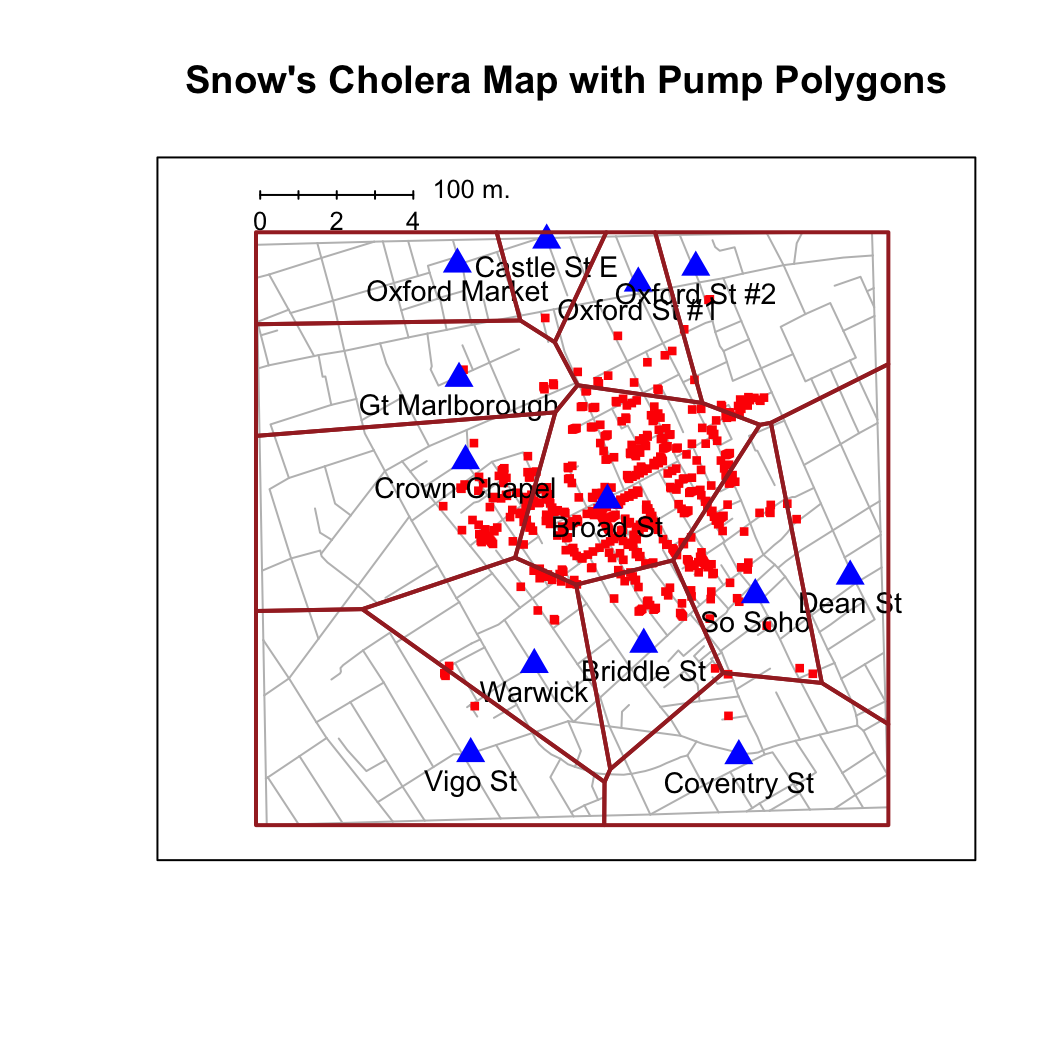
\includegraphics[width=0.6\linewidth]{05-observational_files/figure-latex/pump-1} 

}

\caption{Deaths (red dots) and pump locations.  Polygons that surround
each pump enclose the locations for which that is the nearest pump.}\label{fig:pump}
\end{figure}

Snow noted that ``Within 250 yards of the spot where Cambridge Street joins Broad Street there were upwards of 500 fatal attacks of cholera in 10 days\ldots{}''. By contrast, none of the employees of a local Soho brewery developed cholera. The reason, he judged, was that they drank water from the brewery (which had a different source from the Broad St pump) or just drank beer alone.\\
Coleman (\citeproc{ref-coleman2019causality}{2019}) gives detailed comments on Snow's work.

New Zealand cities had similar issues from the 1840s and 1850s through until~the end of the century, arising from failures to install proper drainage systems.\footnote{See Christine Dann: `Sewage, water and waste - Stinking cities', Te Ara - the Encyclopedia of New Zealand, (8 June 2017) \url{https://teara.govt.nz/en/zoomify/24431/dunedin-renamed-stinkapool}}

\section{Are there missing explanatory factors?}\label{sec:maternity}

The (\citeproc{ref-wernham_EtAl_2016}{Wernham et al. 2016}) study used data from 244,047 singleton term deliveries that occurred between 2008 and 2012 to make the claim that midwife led care, as opposed to medical led care, gave a greater risk of adverse fetal and neonatal outcomes. Notably, the claim was that midwife led care resulted in a lower Apgar score (a measure of infant health immediately after birth) and a greater risk of the imprecisely defined diagnosis of birth asphyxia.

This study was then the basis for exaggerated claims in an article in the October 8-14 2016 issue of the NZ Listener (\citeproc{ref-chisholm_2016}{Chisholm 2016} ``Birth Control''). Contrary to what was claimed, the research did not ``lob a grenade into the historically war-torn territory of New Zealand's maternity care.'' Even less did its results warrant the melodramatic claims of ``Alarming maternity research'' and ``Revolution gone wrong'' that appeared on the Listener's front cover.

A major~issue with the analysis is that it relies on using the NZ Deprivation Index\footnote{\url{https://www.health.govt.nz/publication/nzdep2013-index-deprivation}} to adjust for socioeconomic differences. This provides a deprivation score for meshblocks, each of around 60--110 people. It estimates the relative socioeconomic deprivation of an area, and does not directly relate to individuals. Deprived areas will often include some individuals with high socioeconomic status. Caesarean section, as a delivery type, may well have been more accessible for those of higher socioeconomic status. For National Women's in Auckland, the elective Caesarean rate at term over 2006-2015 for doctor-led care was 32.8\%, as against 7.4\% for self employed midwives (\citeproc{ref-farquhar2016letter}{Farquhar, McCowan, and Fleming 2016}). Effects from fetal alcohol syndrome were not accounted for, nor were direct effects from substance abuse. International data indicates that fetal alcohol syndrome may affect as many as 3\% of births.\footnote{\url{https://www.health.govt.nz/our-work/diseases-and-conditions/fetal-alcohol-spectrum-disorder}}

Studies that are similarly relatively carefully done, but naive in the weight placed on the regression results, are embarrassingly common. There are analysis tools, and associated graphs, that the authors of the study could and should have used to shed light on the likely effectiveness of the adjustments made for differences between the two groups, other than whether the delivery was midwife led or medical led.

\section{The uses and traps of rule-based methods}\label{the-uses-and-traps-of-rule-based-methods}

Figure \ref{fig:seeSpam} shows the distributions of values of six variables that have been selected for use for present illustrative purposes, from an historical dataset (pre 1999, now long past its ``use by'' date) that has data on 4601 email messages, of which 1813 were identified as spam. In practical use, such datasets have to be continually updated as spammers change their strategies

\begin{figure}[H]

{\centering 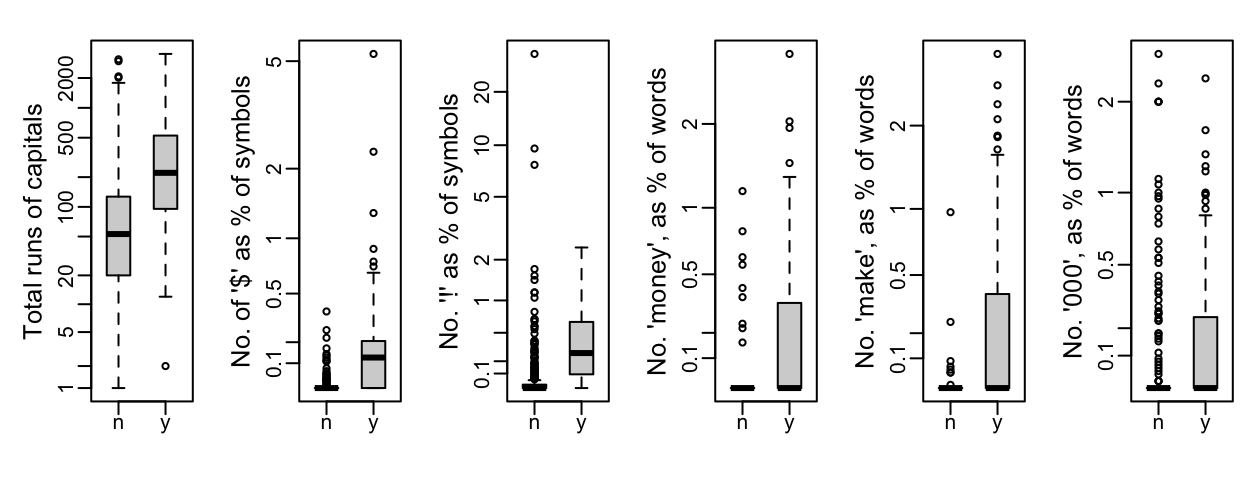
\includegraphics{05-observational_files/figure-latex/seeSpam-1} 

}

\caption{Boxplots, showing distribution of variable values
               in data used to predict email spam}\label{fig:seeSpam}
\end{figure}

Two types of decision tree approaches will be discussed --- the use of individual decision trees, and the random forest approach which generates and uses large numbers of trees in the decision making process.

Figure \ref{fig:spam} shows a decision tree that has been derived for the spam data.

\begin{figure}[H]

{\centering 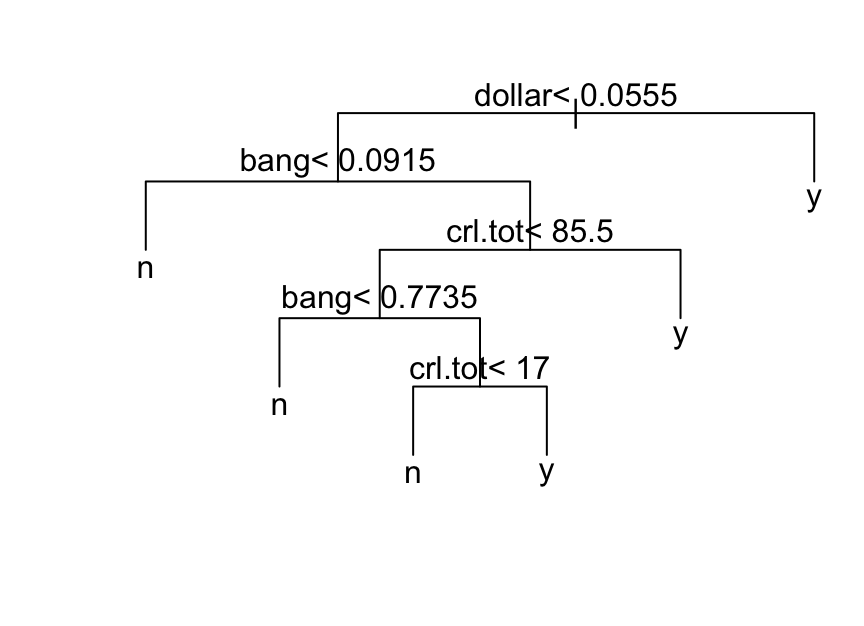
\includegraphics[width=0.48\linewidth]{05-observational_files/figure-latex/spam-1} 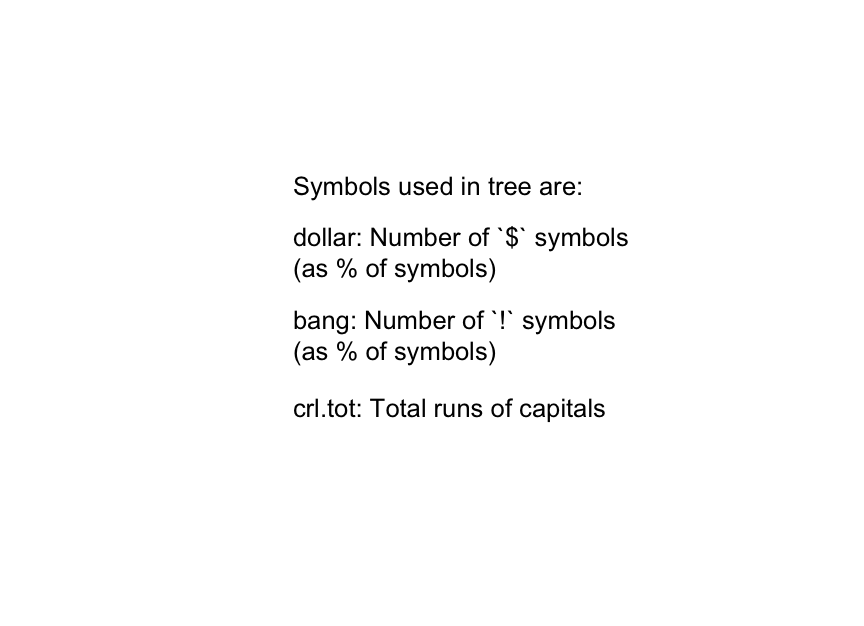
\includegraphics[width=0.48\linewidth]{05-observational_files/figure-latex/spam-2} 

}

\caption{Decision tree for spam data. If the condition is satisfied, take
               the branch to the left.  Otherwise, take the branch to the right.}\label{fig:spam}
\end{figure}

The tree in Figure \ref{fig:spam} would be too inaccurate for practical use, even suitably updated with new data, but it is easy to follow the decsion tree process.

\subsection*{From trees to forests}\label{from-trees-to-forests}
\addcontentsline{toc}{subsection}{From trees to forests}

``Random forests'' improve on decision trees by using samples from the data to create a forest (a ``random forest'') of trees, then voting between the trees. A downside is that ``Random forests'' and similar methods operate largely as black boxes. For detection of spam email, this may, as those who deploy the spam detectors have little idea what may be going on in the minds of the spammers, not be too much of an issue. One wants a spam detector that will respond effectively to whatever is thrown at it.

\subsection*{It helps to know the how and why of the algorithms used}\label{it-helps-to-know-the-how-and-why-of-the-algorithms-used}
\addcontentsline{toc}{subsection}{It helps to know the how and why of the algorithms used}

Both decison trees and random forests follow an \emph{algorithmic} process. The relatively ``black box'' nature of the random forest approach places an especially strong burden on the analyst to ensure relevant data have been used, and that the algorithm really is doing its intended task. In her book ``Weapons of math destruction'', O'Neil (\citeproc{ref-oneil_2016}{2016}) comments:

\begin{quote}
\ldots{} it's not enough to just know how to run a black box algorithm. You actually need to know how and why it works, so that when it does'nt work, you can adjust.
\end{quote}

This is too strong. But if one does not know the how and why of how an algorithm works, it is absolutely crucial to be sure that the data used to fit and test the model (the ``training''~and ``test'' data) are directly relevant to the task in hand.

Automated systems that can be easily gamed do, however, abound. They are a menace!

\chapter{Weighting effects that skew statistics}\label{sec:yule1}

\section{Covid-19 deaths --- comparing countries}\label{covid-19-deaths-comparing-countries}

\begin{figure}[H]

{\centering 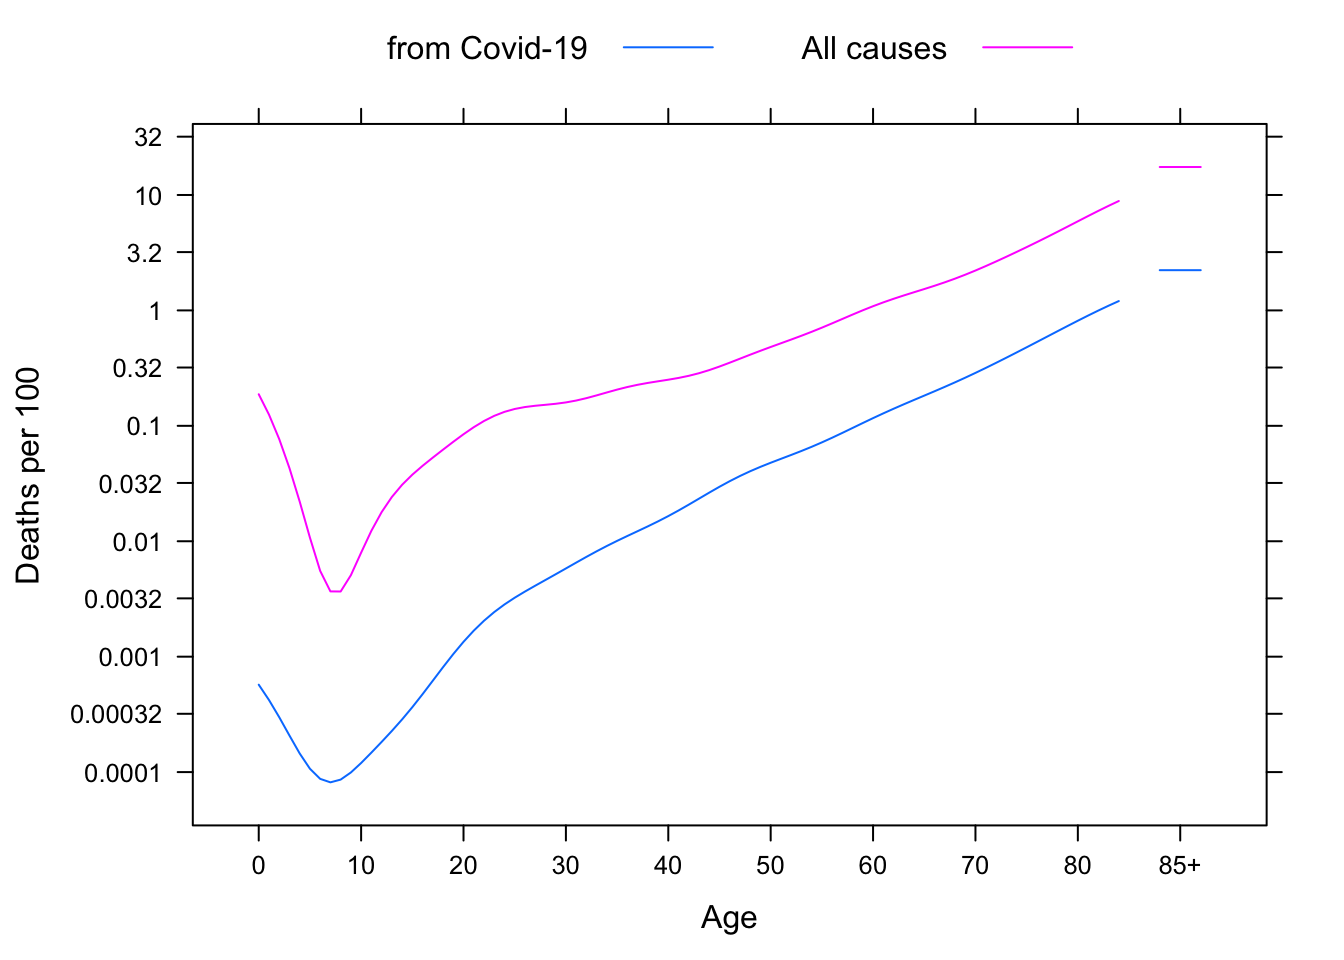
\includegraphics[width=0.6\linewidth]{06-weighting_files/figure-latex/riskByAge-1} 

}

\caption{US data for proportions who died from Covid-19, and in total,
for the 13 months up to 31 January 2021. Vaccination of a substantial 
part of the population, and the emergence of new variants, will,
six months or more later, have substantially changed the pattern
of relative risks by age.}\label{fig:riskByAge}
\end{figure}

Figure \ref{fig:riskByAge} shows stark differences by age in US Covid-19 death rates. The US death rates per 1000 for under age 65 as opposed to age \(>=\) 65, were 0.28, 6.3 US totals for infection rates and for hospital admissions were also impacted by age structure, but to a lesser extent. More recent Covid-19 variants would present a somewhat different picture.

Countries with a lower proportion of their population aged \textgreater=65 would, if the death rates for each of the two groups are similar to US rates, have lower overall death rates. The following compares the overall deaths rates for the US with what might, if these figures carried across, be expected for Kenya and for Italy.

\begin{verbatim}
                               US Italy Kenya
Percentage 65 or more        16.3  23.3   2.5
Expected deaths per 100,000 126.7 168.5  43.5
Reported deaths per 100,000 126.7 146.0   3.3
\end{verbatim}

Between country comparisons are hazardous. The dependence of reported case numbers on testing rates and reporting protocols makes it likely that they will be substantial undercounts, to an extent that varies from country to country.

\section{University admissions data --- Simpson's paradox}\label{sec:Y-S}

Admissions data for University of California Berkeley in 1973 showed a curious anomaly. Overall admission rates strongly favoured males, while in individual departments the rates mostly favoured females. The table shows percent admission rates, with number applying shown in brackets underneath.

\begin{tabular}{l>{\raggedleft\arraybackslash}p{5em}>{\raggedleft\arraybackslash}p{2.5em}>{\raggedleft\arraybackslash}p{2.5em}>{\raggedleft\arraybackslash}p{2.5em}>{\raggedleft\arraybackslash}p{2.5em}>{\raggedleft\arraybackslash}p{2.5em}>{\raggedleft\arraybackslash}p{2.5em}}
\toprule
  & OVERALL & A & B & C & D & E & F\\
\midrule
Male & \textbf{44.5} & 62.1 & 63 & 36.9 & 33.1 & 27.7 & 5.9\\
 & \textbf{(2691)} & (825) & (560) & (325) & (417) & (191) & (373)\\
Female & \textbf{30.4} & 82.4 & 68 & 34.1 & 34.9 & 23.9 & 7\\
 & \textbf{(1835)} & (108) & (25) & (593) & (375) & (393) & (341)\\
\bottomrule
\end{tabular}

Figure \ref{fig:UCBgph1} provides a graphical summary.

\begin{figure}[H]

{\centering 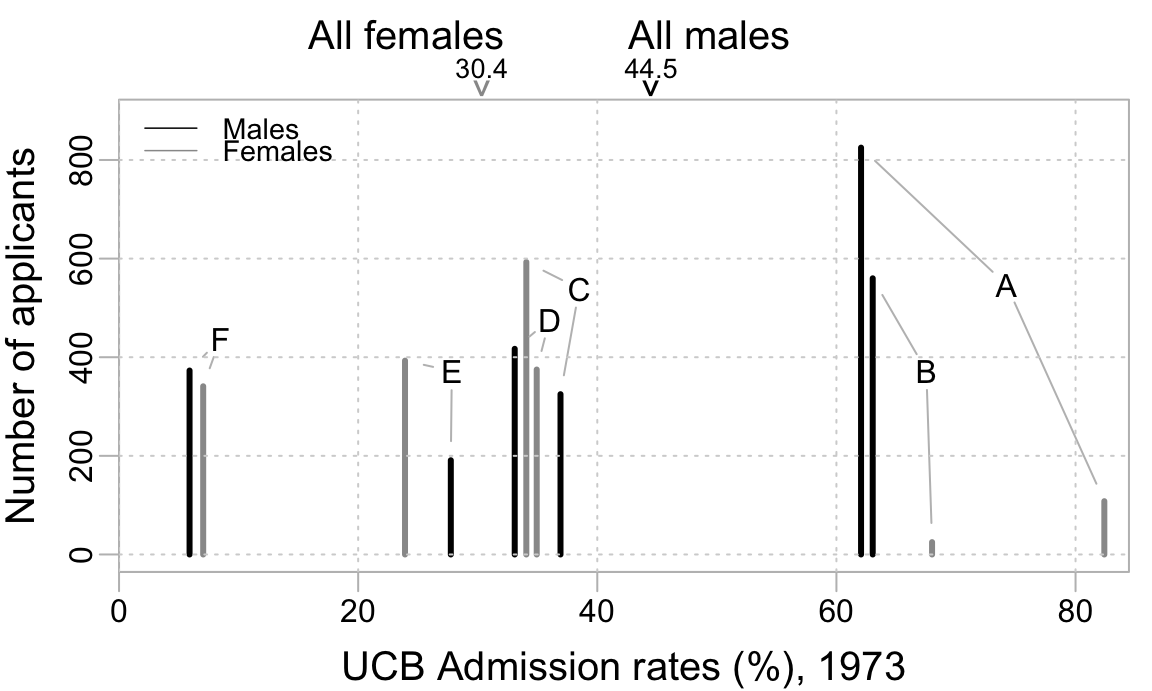
\includegraphics[width=0.72\linewidth]{06-weighting_files/figure-latex/UCBgph1-1} 

}

\caption{UCB admossion data for 1973, for males and females, by 
department.  Department labels range from A to E.  Notice that
the largest differences in admission rates are for departments
A and B, in both cases favouring females.}\label{fig:UCBgph1}
\end{figure}

There are thus three different broad admission patterns. The big differences in admission rates were in departments A (82.4\%-62.1\%=20.3\%) and B (68\%-63\%=5\%), in both cases favouring females. In the other four departments, differences were 3.8\% or less, and split very nearly equally between slightly favouring females and slightly favouring males. Also, the relative numbers of males and females applying did not show the same big differences as in departments A and B.

\begin{table}[H]
\centering
\caption{Comparion of admission rates (percent) and numbers of males and
females applying, for departments A, B, and CDEF which combines 
numbers for departments other than A and B.}
\centering
\begin{tabular}[t]{l>{\raggedleft\arraybackslash}p{5em}>{\raggedleft\arraybackslash}p{2.25em}>{\raggedleft\arraybackslash}p{2.25em}>{\raggedleft\arraybackslash}p{2.25em}}
\toprule
  & TOTALS & A & B & CDEF\\
\midrule
Male & \textbf{44.5} & 62.1 & 63 & 25.5\\
 & \textbf{(2691)} & (825) & (560) & (1306)\\
Female & \textbf{30.4} & 82.4 & 68 & 26.5\\
 & \textbf{(1835)} & (108) & (25) & (1702)\\
\bottomrule
\end{tabular}
\end{table}

\begin{itemize}
\tightlist
\item
  The overall male rates are weighted (825+560):(325+(417+191+373 = 1385:1306 or 1.06:1, between an overall AB rate of 62.5\%, and the CDEF rate of 25.5\%.\\
\item
  Overall female rates are weighted 133:1702 = 1:15.8 for departments A and B, as against departments CDEF. Overall female rates are, accordingly, strongly weighted towards the 26.5\% rate for other departments.
\end{itemize}

\subsection*{UCB Admissions Data -- Another perspective}\label{ucb-admissions-data-another-perspective}
\addcontentsline{toc}{subsection}{UCB Admissions Data -- Another perspective}

\begin{figure}[H]

{\centering 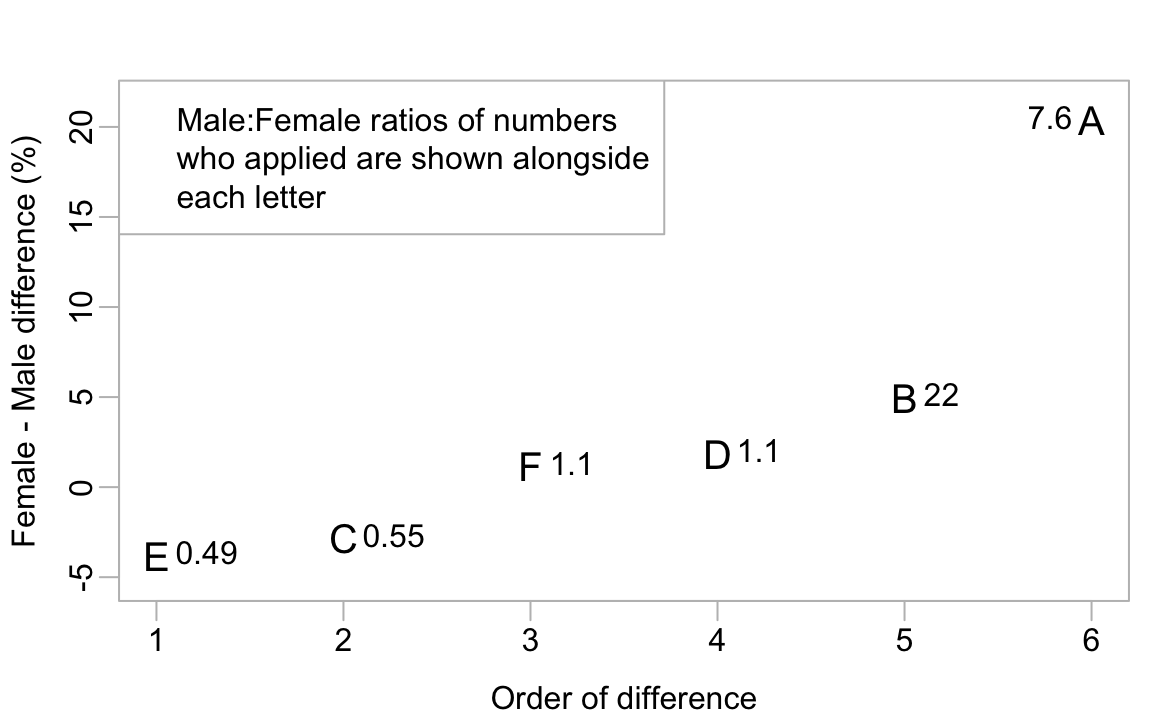
\includegraphics[width=0.72\linewidth]{06-weighting_files/figure-latex/UCBdiffs-1} 

}

\caption{UCB admossion data for 1973 --- another perspective.}\label{fig:UCBdiffs}
\end{figure}

In order to understand how the overall imbalance between numbers of males and females arose, it was necessary to break the data down by department. The major driver of the overall imbalance was the low numbers of females, relative to males, applying to department A (and, to a lesser extent, B) where admission rates were highest.

See \url{https://www.youtube.com/watch?v=ZDinnCwP3dg} for an animated video that explains the Yule-Simpson paradox.

\subsection*{A note on Lord's paradox}\label{a-note-on-lords-paradox}
\addcontentsline{toc}{subsection}{A note on Lord's paradox}

The same sorts of paradoxical effects can be found in regression. The Yule-Simpson paradox may be regarded as a special case of Lord's paradox, described in Lord (\citeproc{ref-lord1967paradox}{1967}).\footnote{See also Tu and Gilthorpe (\citeproc{ref-tu2011statistical}{2011}), pp.60-71} Any attempt to attach meaning to regression coefficients can be highly misleading, unless it is clear that effects of all relevant variables are properly accounted for. It is rarely easy, with observational data, to be sure that this has been done effectively, a point that will be taken up in Chapter \ref{sec:reg}.

\section{Comparing unvaccinated with vaccinated}\label{comparing-unvaccinated-with-vaccinated}

Once high enough vaccination rates have been achieved, a greater number of Covid-19 infections will be found among the vaccinated than among the vaccinated. Suppose that, for a particular age group and for a particular vaccine, the risk rate for severe Covid-19, is 5\% for unvaccinated versus 1\% for vaccinated, i.e.~a relative risk of 5:1. Consider the following scenarios. The final column has the relative numbers, for unvaccinated versus vaccinated with Covid-19:

\begin{longtable}[]{@{}lll@{}}
\toprule\noalign{}
Unvaccinated & Vaccinated & Relative numbers with severe Covid-19 \\
\midrule\noalign{}
\endhead
\bottomrule\noalign{}
\endlastfoot
200 & 800 & 10 unvaccinated : 8 among vaccinated \\
100 & 900 & 5 : 9 \\
0 & 1000 & 0 : 10 \\
\end{longtable}

At a certain point, provided the risk ratio is greater than 1.0, the higher number will be from the vaccinated. Of course, the 100\% vaccination rate scenario in the final row is unlikely to~be realized.

\subsection*{Report found almost 60\% of~cases were vaccinated}\label{report-found-almost-60-of-cases-were-vaccinated}
\addcontentsline{toc}{subsection}{Report found almost 60\% of~cases were vaccinated}

As of August 15 2021, Israeli data showed that 301 of those hospitalized with severe Covid-19 were fully vaccinated, while 214 were not. We need to compare, not the counts, but the proportions of vaccinated and unvaccinated, i.e., look at the percentages that are shown in brackets following the counts.\footnote{Data are from \url{https://bit.ly/3h1mwXQ}, on the website \url{https://www.covid-datascience.com/}.} Numbers given are of~those aged 12 or more.

\begin{longtable}[]{@{}llll@{}}
\toprule\noalign{}
& Unvaccinated & Fully vaccinated & \\
\midrule\noalign{}
\endhead
\bottomrule\noalign{}
\endlastfoot
Number (aged \textgreater=12) & 1,302,912 & 5,634,634 & \\
Severe cases & 214 (16.4\%) & 301 (5.3\%) & \\
\end{longtable}

The relative risk is 16.4/5.3 \(\simeq\) 3.1. Because no account has been taken of age differences, this still underestimates the effectiveness of vaccination. A fairer picture is:

\begin{longtable}[]{@{}llll@{}}
\toprule\noalign{}
& Unvaccinated & Fully vaccinated & \\
\midrule\noalign{}
\endhead
\bottomrule\noalign{}
\endlastfoot
Number \textless50 & 1,116,834 & 3,501,118 & \\
Severe cases & 43 (3.9\%) & 11 (0.3\%) & \\
---- & ---- & ---- & \\
Number \textgreater=50 & 186,078 & 2,133,518 & \\
Severe cases & 171 (91.9\%) & 290 (13.6\%) & \\
\end{longtable}

The relative risk is 3.9/0.3 \(\simeq\) 13 for those under 50, and 91.9/13.6 \(\simeq\) 6.8 for those over 50, i.e., in both cases much greater than the 3.1 ratio obtained when the split between under 50s and 50 or more is ignored. Even this does not do justice to the data, which needs to be split into smaller age ranges.

\section{Further illustrative examples}\label{further-illustrative-examples}

\subsection*{Does Baclofen help in reducing pain?}\label{does-baclofen-help-in-reducing-pain}
\addcontentsline{toc}{subsection}{Does Baclofen help in reducing pain?}

\begin{figure}[H]

{\centering 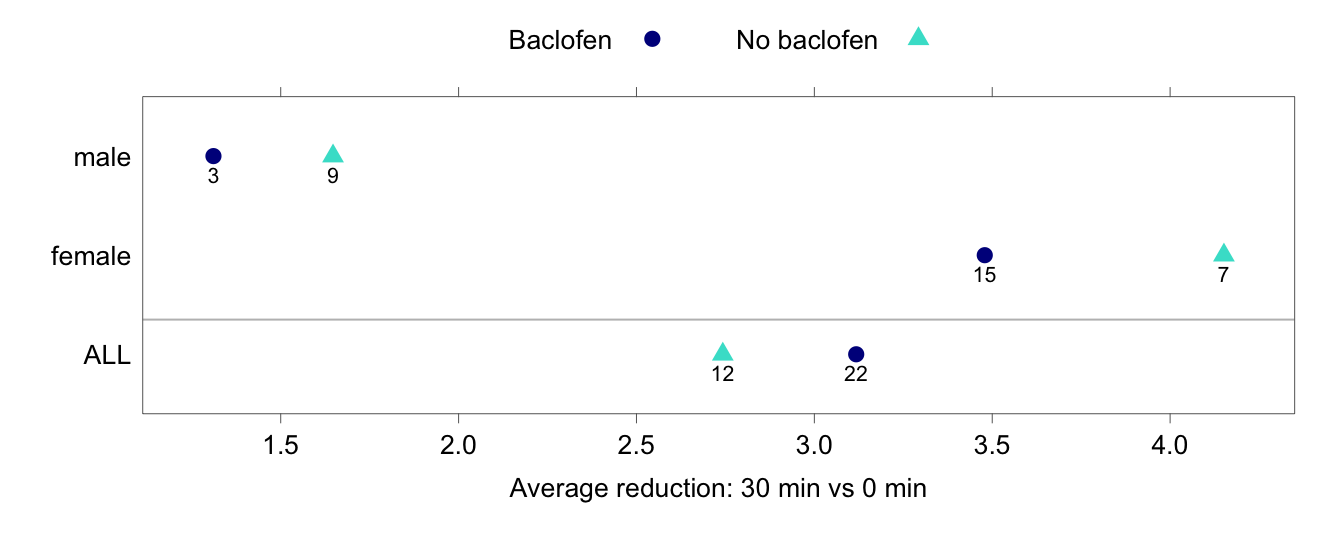
\includegraphics{06-weighting_files/figure-latex/painkiller-1} 

}

\caption{Data are pain reduction scores. Subgroup numbers, shown
    below each point, weight the overall average (''ALL'') for
    baclofen towards the high female average, and for no baclofen
    slightly towards the low male average.}\label{fig:painkiller}
\end{figure}

In work reported in Cohen (\citeproc{ref-cohen1996}{1996}), researchers were comparing two analgesic treatments, without and with baclofen. When the paper was first submitted for publication, an alert reviewer spotted that some of the treatment groups contained more women than men, and asked whether this might account for the results.

For a fair overall comparison:

\begin{itemize}
\tightlist
\item
  Calculate means for each subgroup separately.
\item
  Overall treatment effect is average of subgroup differences.
\end{itemize}

The effect of baclofen (reduction in pain score from time 0) is then:

\begin{itemize}
\tightlist
\item
  Females: 3.479 - 4.151 = -0.672 (-ve, therefore an increase)
\item
  Males: 1.311 - 1.647 = -0.336
\item
  Average, male \& female = -0.5 \(\times\) (0.672+0.336) = -0.504
\end{itemize}

\subsection*{Web page revenue per click}\label{web-page-revenue-per-click}
\addcontentsline{toc}{subsection}{Web page revenue per click}

Smith (\citeproc{ref-smith-sd}{2014}) (p.111) describes an experiment where a US Internet company collected data that compared the effectiveness of two strategies. In the 1-click strategy, an advert appeared on the website's first page. The 2-click strategy required the user to click on a keyword which then led to a page with the advert. The response (total dollar value of purchases) was compared between the two.

The following, with numbers changed to make the comparison relatively simple, shows a scenario that is not unlike that given by Smith:

\begin{longtable}[]{@{}llllllll@{}}
\toprule\noalign{}
1-click & & & & 2-click & & & \\
\midrule\noalign{}
\endhead
\bottomrule\noalign{}
\endlastfoot
Revenue & Users & RP1000 & & Revenue & Users & RP1000 & \\
\$2500 & 200 & \$12.50 & & \$3000 & 300 & \$15.00 & \\
\end{longtable}

The 1-click strategy appears to give a better return.

Now, see how the numbers divide up when a split is made between US and international visitors to the site. The numbers (thousands) for the two strategies divide up thus, with the revenue per thousand users given, in each case, in brackets:

\begin{longtable}[]{@{}lll@{}}
\toprule\noalign{}
& 1-click & 2-click \\
\midrule\noalign{}
\endhead
\bottomrule\noalign{}
\endlastfoot
US & 50 & 80 \\
& (\$32) & (\$30) \\
Int & 150 & 120 \\
& (\$6) & (\$5) \\
\end{longtable}

The 1-click strategy clearly gives a better return, both for US and for international users.

The overall figure is dominated by the result for the 150,000 international users (as opposed to 50,000 US) in the 1-click sample. This compares with the much weaker weighting towards international users (120,000 as opposed to 80,000) in the 2-click sample.

In the case that Smith reported, the type of analysis shown was followed up with a randomized experiment (an A/B test), where the probability of assignment to 1-click, as opposed to 2-click, was the same for both classes of user.

\section{Cricket Bowling Averages}\label{cricket-bowling-averages}

\subsection*{\texorpdfstring{Runs (R), wickets (W) and runs per wicket (\{\em RPW\})}{Runs (R), wickets (W) and runs per wicket (\{\})}}\label{runs-r-wickets-w-and-runs-per-wicket}
\addcontentsline{toc}{subsection}{Runs (R), wickets (W) and runs per wicket (\{\em RPW\})}

\vspace*{-8pt}

\begin{center}
\begin{tabular}{lrrr||rrr||rrr}
\hline
 & \multicolumn{3}{c}{1st innings} & \multicolumn{3}{c}{2nd innings} &
\multicolumn{3}{c}{Overall} \\
\cline{2-4} \cline{5-7} \cline{8-10}
& R & W & {\em RPW}   & R & W & {\em RPW} & R & W
& {\em RPW}\\
Bowler A & 40 & 4 & {\em 10.0} & 240 & 6 & {\em 40.0} & 280 & 10 &
{\em 28.0}\\
Bowler B & 70 & 5 & {\em 14.0} & 50 & 1 & {\em 50.0} & 120 & 6 & {\em 20.0} \\
\hline
\end{tabular}
\end{center}

\subsection*{\texorpdfstring{Fair comparison: Compare runs per wicket (\{\em RPW\})}{Fair comparison: Compare runs per wicket (\{\})}}\label{fair-comparison-compare-runs-per-wicket}
\addcontentsline{toc}{subsection}{Fair comparison: Compare runs per wicket (\{\em RPW\})}

\vspace*{-5pt}

\begin{center}
\begin{tabular}{lrr||rr||rr}
\hline
 & \multicolumn{2}{c}{1st innings} & \multicolumn{2}{c}{2nd innings} &
\multicolumn{2}{c}{Overall} \\
\cline{2-3} \cline{4-5} \cline{6-7}
         &  RPW & {\em W}   &  RPW & {\em W} &
           RPW & {\em W} \\[4pt]
Bowler A &  10.0 & (4) & 40.0 & (6)  &
$\frac{10+40}{2} = 25$ & (10)\\[4pt]
Bowler B & 14.0 & (5)  & 50.0 & (1) & $\frac{50+14}{2} = 32$  &  (6)\\[4pt]
\cline{2-3} \cline{4-5} \cline{6-7}
\end{tabular}
\end{center}

\section{Epistatic effects in genetic studies}\label{epistatic-effects-in-genetic-studies}

In population genetics, Simpson's paradox type effects are known as epistasis. Most human societies are genetically heterogeneous. In San Francisco, any gene that is different between the European and Chinese populations will be found to be associated with the use of chopsticks! If a disease differs in frequency between the European and Chinese populations, then a naive analysis will find an association between that disease and any gene that differs in frequency between the European and Chinese populations.

Such effects are major issues for gene/disease population association studies. It is now common to collect genetic fingerprinting data that should identify major heterogeneity. Providing such differences are accounted for, large effects that show up in large studies are likely to be real. Small effects may well be epistatic.

\chapter{Matters of consequence}\label{matters-of-consequence}

\section{\texorpdfstring{\href{https://en.wikipedia.org/wiki/MMR_vaccine_controversy}{The MMR vaccine scandal}}{The MMR vaccine scandal}}\label{the-mmr-vaccine-scandal}

The MMR vaccine was developed to for~use in preventing measles, mumps, and rubella. Andrew Wakefield was the lead author of a study published in 1998, based on just twelve children, that claimed to find indications of a link between the MMR vaccine and autism. The journalist Brian Deer had a key role in identifying issues with the work,~including fraudulent manipulation of~the medical~evidence.

It emerged that

\begin{itemize}
\tightlist
\item
  Wakefield had multiple undeclared conflicts of interest
\item
  Funding came from a group of lawyers who were interested in possible personal injury lawsuits
\item
  From 9 children said to have regressive autism

  \begin{itemize}
  \tightlist
  \item
    Only 1 had been diagnosed; 3 had no autism
  \item
    5 had developmental problems before the vaccine
  \end{itemize}
\end{itemize}

Wakefield's 1998 claims were widely reported

\begin{itemize}
\tightlist
\item
  Vaccination rates in the UK and Ireland dropped sharply
\item
  The incidence of measles and mumps increased, resulting in deaths and in severe and permanent injuries.
\end{itemize}

Wakefield was found guilty by the General Medical Council of serious professional misconduct in May 2010 and was struck off the Medical Register.\\
Following the initial claims in 1998, multiple large epidemiological studies failed to find any link between MMR and autism.

Fact boxes on the Harding site summarize evidence of the effectiveness of the \href{https://www.hardingcenter.de/de/search/node?keys=mmr}{MMR vaccine}\footnote{\url{https://www.hardingcenter.de/de/search/node?keys=mmr}}

\section{Sally Clark's disturbing cot death story}\label{sally-clarks-disturbing-cot-death-story}

Sudden Infant Death (SID), also referred to as ``cot death'', is the name given to the unexplained sudden death of very young children. The story of Sally Clark's unfortunate brush with the law, following the death of a second child, is interesting, disturbing, and educational. Sally's experience highlighted ways in which the UK legal system needed to take on board issues that affect the use of medical evidence --- issues of a type that can be important in medical research.

Paediatrician Sir Roy Meadow had argued in his 1997 book \textbf{ABC of Child Abuse} that ``unless proved otherwise, one cot death is tragic, two is suspicious and three is murder.'' Was this an example of ``Too hard! Try something easier, and wrong!'' Or was it the triumph of assumed ``knowledge'' over hard evidence?

Meadow's role as an expert witness for the prosecution in several trials played a crucial part in wrongful convictions for murder. The case that attracted greatest attention is that of Sally Clarke, both of whose children were ``cot death'' victims. Following the death of the second child, Meadow gave evidence at her 1999 trial, and appeal in 2000. Sally Clark was finally acquitted in 2003.

\begin{itemize}
\tightlist
\item
  Meadow gave 1 in 8,500 as cot death rate in affluent non-smoking families

  \begin{itemize}
  \tightlist
  \item
    Squared 8,500 to get odds of 73,000,000:1 against for two deaths.
  \item
    Meadow assumed, wrongly, that the probability of a death from natural causes was the same in all families.
  \item
    A first ``cot death'' is, in some families at least, evidence of a greater proneness to death from natural causes.
  \end{itemize}
\item
  Royal Statistical Society press release: ``Figure has no statistical basis''

  \begin{itemize}
  \tightlist
  \item
    2000 appeal judges: The figure was a ``sideshow'' that would not have influenced the jury's decision.
  \item
    The appeal judges' statement was described by a leading QC, not involved in the case as: ``a breathtakingly intellectually dishonest judgment.''
  \end{itemize}
\item
  2003: It emerged that 2nd death was from bacterial infection

  \begin{itemize}
  \tightlist
  \item
    In a second appeal, Sally Clark was freed.
  \end{itemize}
\item
  2005: Meadow was struck from medical register

  \begin{itemize}
  \tightlist
  \item
    2006: reinstated by appeal court --- misconduct fell short of ``serious''!
  \end{itemize}
\end{itemize}

Meadow was in effect assuming, without evidence, the absence of family-specific genetic or social factors that make cot deaths more likely in some families than in others. Why was Meadow's assumption of independence not challenged in the 1999 trial? Issues of whether or not different pieces of evidence are independent are surely crucial to assessing the total weight of evidence. Meadow had only enough understanding of probability to be dangerous.

Sally Clark was finally acquitted on her second appeal in 2003, with her sense of well-being damaged beyond repair. The forensic evidence had been weak. The web page \url{https://plus.maths.org/content/os/issue21/features/clark/index} has a helpful summary of the statistical issues. It quotes a study that suggests that the probability of a second cot death in the same family is somewhere between 1 in 60 and 1 in 130. Even after this adjustment, the probability of death from natural causes of two children in the same family is low. But so also is the probability that an apparently caring mother from an affluent middle class family, with no history of abuse, will murder two of her own children. Those are the two probabilities that must be compared. Anyone who plans to work as a criminal lawyer ought to understand this crucial point. In a large population, there will from time to time be two deaths from natural causes in the one family.

A small number of appeals were subsequently launched against other convictions where evidence of the same type had been presented, most of them successful. A further consequence was that the law was changed such that no person could be convicted on the basis of expert testimony alone.

The Watkins (\citeproc{ref-watkins2000conviction}{2000}) article ``Conviction by mathematical error?: Doctors and lawyers should get probability theory right'' provides a trenchant critique of the perils of allowing non-statisticians to present unsound statistical arguments, with no effective challenge.

\begin{quote}
Guidelines for using probability theory in criminal cases are urgently needed. The basic principles are not difficult to understand, and judges could be trained to recognise and rule out the kind of misunderstanding that arose in this case.
\end{quote}

Watkins, who was at the time Director of Public Health for Stockport in the UK, argued that the calculation of the relevant probability should have had no regard to the probability of an initial cot death. It surely has some relevance. The basic principles are perhaps~more difficult than Watkins was willing to allow.

\section{The Reinhart and Rogoff saga}\label{the-reinhart-and-rogoff-saga}

Figure \ref{fig:debt2gdp12} plots data, for 1946 -- 2009 from 20 ``advanced'' countries, that underpinned the 2010 paper ``\emph{Growth in Time of Debt}'' by the two Harvard economic historians Reinhart and Rogoff \[RR\].

\begin{figure}[H]

{\centering 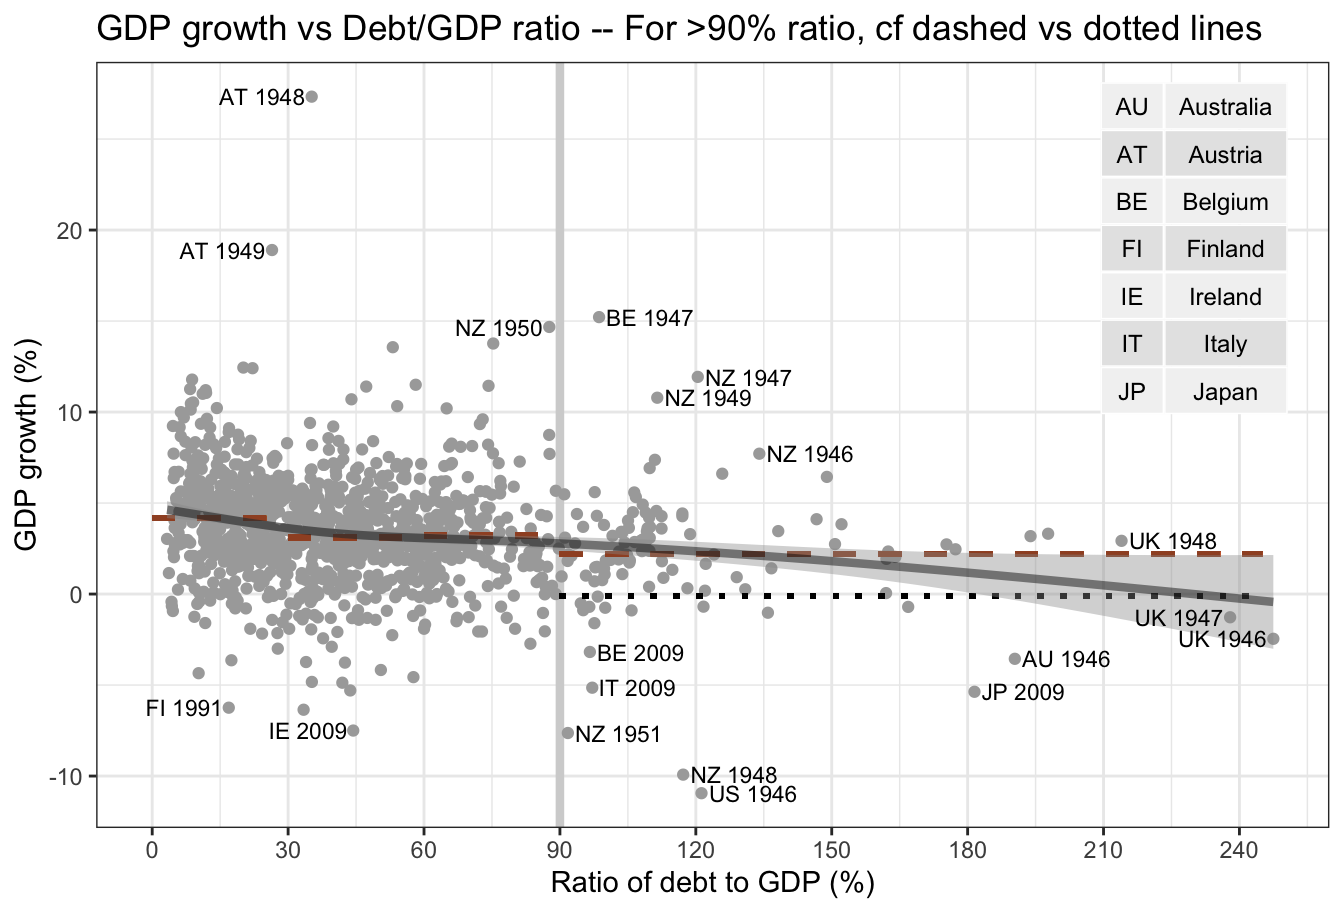
\includegraphics[width=1\linewidth]{07-notable_files/figure-latex/debt2gdp12-1} 

}

\caption{Dashed horizintal lines show means by Debt/GDP category, 
for 20 'advanced' countries, for the years 1946 --- 2009.
(Data are missing for some countries in some years.)
RR's mean (dots) for > 90\% Debt/GDP was from 10 only of the 20. 
The smooth gray curve treats points as independent.}\label{fig:debt2gdp12}
\end{figure}

The paper (\citeproc{ref-reinhart2010growth}{Reinhart and Rogoff 2010}) has been widely quoted in support of economic austerity programs internationally. There was a huge stir, in the media and on the blogosphere, when graduate student Herndon found and published details of coding and other errors in the results that RR had presented.\footnote{\url{http://www.peri.umass.edu/fileadmin/pdf/working_papers/working_papers_301-350/WP322.pdf}}

As well as coding errors, Hendon identified selective exclusion of available data, and unconventional weighting of summary statistics. There was no consideration that the relationship studied has varied substantially by country and over time. Half of the 20 countries had missing data for 5 or more of the years, with the largest number missing in the years 1946 to 1949.

In response to Herndon, Ash, and Pollin (\citeproc{ref-herndon2014does}{2014}) and other critics, Reinhart and Rogoff accepted that coding errors had led to the omission of several countries, but pushed back against other criticisms. Their revised analysis addresses only the most egregious errors in their work. Among other issues, their insistence on treating each data point for each country as an independent piece of evidence makes no sense. The smooth curve fitted in Figure \ref{fig:debt2gdp12} may be regarded as an average over the ten countries, but as Figure \ref{fig:debt2gdp-3} shows, with huge country to~country~variation.

\begin{figure}[H]

{\centering 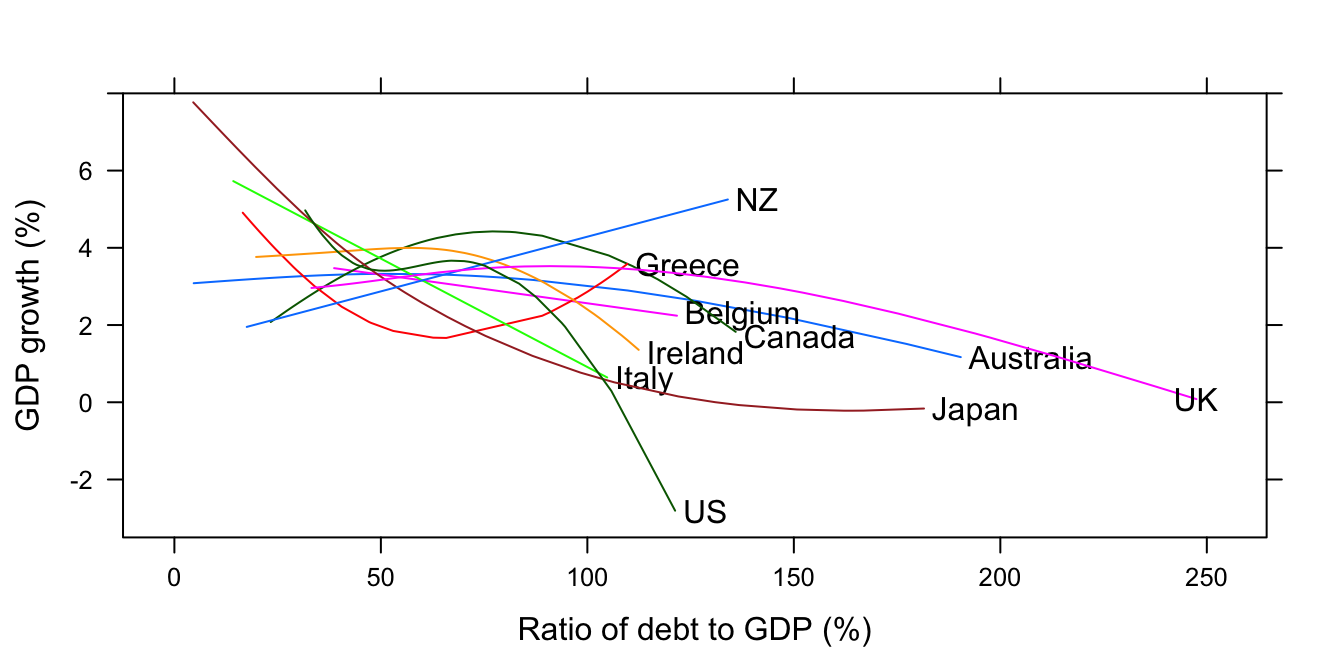
\includegraphics{07-notable_files/figure-latex/debt2gdp-3-1} 

}

\caption{Smooths have been fitted for each of the 10 countries
for which debt to GDP ratios were in some years greater than 90\%.
There is no consistent pattern, as there should be if RR's claim
is to hold up.}\label{fig:debt2gdp-3}
\end{figure}

\subsection*{Is there a pattern across countries?}\label{is-there-a-pattern-across-countries}
\addcontentsline{toc}{subsection}{Is there a pattern across countries?}

There were just 10 countries where debt to GDP ratios were greater than 90\% for one or more years. For 9 of those countries, the average of their GDP growth in the years at issue was on average positive relative to the previous year. The average percentage growth over all 10 countries, weighted according to number of years, was 2.168.

\subsection*{There are further serious issues of interpretation}\label{there-are-further-serious-issues-of-interpretation}
\addcontentsline{toc}{subsection}{There are further serious issues of interpretation}

\begin{itemize}
\tightlist
\item
  Does GDP drive debt/GDP ratio, or is it the other way round?

  \begin{itemize}
  \tightlist
  \item
    Or does a third factor drive both?
  \end{itemize}
\item
  Is the effect immediate, or on future economic performance
\end{itemize}

Smith (p.64) refers to work indicating that economic performance is more closely correlated with economic growth in the past than with future growth.

\subsection*{Parting comments}\label{parting-comments}
\addcontentsline{toc}{subsection}{Parting comments}

Herndon, Ash, and Pollin (\citeproc{ref-herndon2014does}{2014}) comment

``\ldots{} RR's findings have served as an intellectual bulwark in support of austerity politics. The fact that RR's findings are wrong should therefore lead us to reassess the austerity agenda itself in both Europe and the United States.''

The saga emphasizes the importance of working with reproducible code, rather than with spreadsheet calculations. The errors in RR's calculations were from one perspective fortunate. Once highlighted, the errors drew critical attention to the paper, and to the serious flaws in the analysis.

\section[What do malaria drugs do to Covid-19 patients?]{\texorpdfstring{What do malaria drugs do to Covid-19 patients?\footnote{Lancet, May 2020, \url{https://bit.ly/3xqncMt}}}{What do malaria drugs do to Covid-19 patients?}}\label{sec:lancet}

Thirteen days after it was published on May 20 2020, three of the four authors withdrew a paper that claimed to~find that malaria drugs, when used experimentally with patients with Covid-19, led to around 30\% excess deaths. Irrespective of the problems with the data that will be noted shortly, serious flaws in the analysis ought to~have attracted the attention of referees. There was inadequate adjustment for known and measured confounders (disease severity, temporal effects, site effects, dose used).

The study claimed to~be based on data from 96,032 hospitalized COVID-19 patients from six continents, of which 66\% were from North America. Very soon after it appeared, the article attracted critical attention, with a number of critics joining together to submit the Watson et al. (\citeproc{ref-watson2020open}{2020}) letter to Lancet.

The sources from which the data had been obtained could not be verified, data that claimed to be from just five Australian sources had more cases than the total of Australian government figures, and similarly for Australian deaths, there were implausibly small reported variances in baseline variables, mean daily doses of hydroxychloroquine that were 100 mg higher than US FDA recommendations.

Randomized trials designed to test the effectiveness of the drugs, and that were in progress at the time when the paper appeared, were temporarily halted. The eventual~conclusion was that the drugs did not improve medical outcomes. There was some evidence that hydroxychloroquine could have adverse effects.

With current web-based technology, randomized controlled trials can be planned and carried out and yield definitive answers, in much the same time as it would take to collect and analyze the data that are required for an observational study whose conclusions can be, at best, suggestive. Data confidentiality issues are easier to handle in the context of an RCT.

\section{A simplistic use of publicly available data}\label{a-simplistic-use-of-publicly-available-data}

A June 2021 paper in \emph{Vaccines}, titled ``The Safety of COVID-19 Vaccinations -\/--- We Should Rethink the Policy.''\footnote{\emph{Vaccines}, June 2021, bit.ly/3dTg1oh} massively over-stated vaccine risk. The paper claimed that ``For three deaths prevented by vaccination we have to accept two inflicted by vaccination.''

\begin{itemize}
\tightlist
\item
  Deaths were from any cause, post-vaccination, reported both by professionals and the public\\
  (Such data has to~be used with a `baseline' comparison)
\item
  Vaccine benefits extend far beyond 6 weeks of Israeli study
\item
  The paper focused on immediate risk to individual, not community.
\item
  The way that any risk from the vaccine balances out against risk of death from Covid-19 will vary depending on the the age structure of the population, on proportion immunized within each age group, and on the age and health of the individual.
\end{itemize}

Deaths that could be verified as from the Pfizer vaccine have been, with the possible exception of frail elderly people, extremely rare. See US CDC report on risk (for Pfizer, anaphylaxis)\footnote{www.cdc.gov/coronavirus/2019-ncov/vaccines/safety/adverse-events.html}, and Helen Petousis-Harris' commentary on risks.\footnote{sciblogs.co.nz/diplomaticimmunity/2021/04/15/covid-vaccines-and-blood-clots-what-is-this-about/}

\chapter{Regression and Correlation}\label{sec:reg}

When two variables show a relationship, they are said to be correlated. Regression and correlation offer alternative, and complementary, perspectives on the relationship.\footnote{The discussion will avoid the technicalities of alternative ways to measure correlation. The particular correlation measure that is used in the examples that follow is the product-moment or Pearson correlation, which relates directly to linear (straight line) regression.} Nonsense correlations that arise where the third variable is time provide simple examples.\footnote{Yule-Simpson type effects, discussed in Section \ref{sec:yule1}, are important in a regression context also.}

\section{Correlation is not causation}\label{correlation-is-not-causation}

Variable A may cause variable B. Or variable B may cause variable A. Or both A and B may be caused (or driven) by a third variable C.

The following are examples where causation likely goes in the other direction, or where a third variable is likely to be involved. Such examples help highlight how correlation can and cannot reasonably be interpreted.

\begin{enumerate}
\def\labelenumi{\arabic{enumi}.}
\tightlist
\item
  Children of parents who try to control eating are more likely to be overweight.
\item
  Ice cream consumption \& polio were closely correlated in the 1950s.

  \begin{itemize}
  \tightlist
  \item
    Summer was when the virus thrived.
  \end{itemize}
\end{enumerate}

Cases where the third variable is time, as in Figure \ref{fig:socAnti}, are a fruitful source of examples of spurious correlations.\footnote{Figure \ref{fig:socAnti} is one of many such examples that are available from\\
  \url{http://www.tylervigen.com/spurious-correlations}.} Is there a third factor, or is this just a chance relationship?

\begin{figure}

{\centering 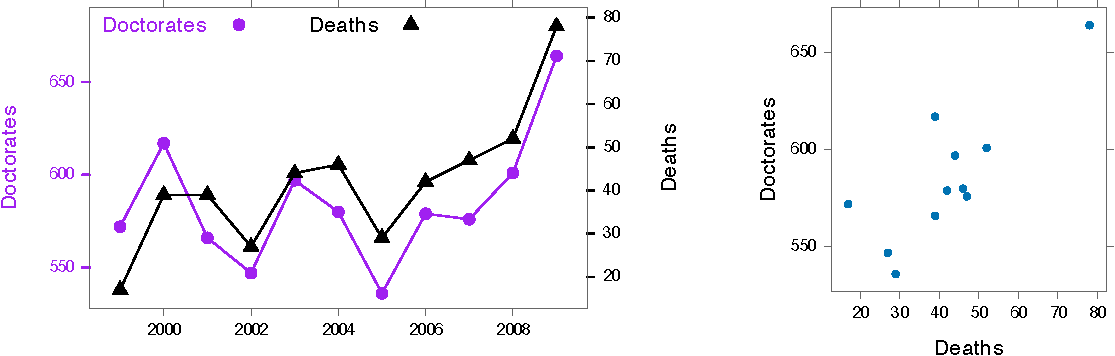
\includegraphics[width=1\linewidth]{08-regress_files/figure-latex/socAnti-1} 

}

\caption{Sociology PhDs awarded (from US National Science 
Foundation data) vs Deaths from Anticoagulants.  Notice
that `Doctorates` and `Deaths` show a very similar pattern
of change from year to year.}\label{fig:socAnti}
\end{figure}

Another example is that, over 1997 to 2009, US Sociology PhDs awarded correlated strongly with worldwide non-commercial space launches. These correlations would seem to be the result of chance. Look at enough variable pairs, and such correlatiosn will sometimes appear.

\section{Regression to the mean}\label{regression-to-the-mean}

Tall fathers are likely to have tall sons, but shorter than themselves. Tall sons are likely to have tall fathers, but shorter than themselves. The data shown in Figure \ref{fig:pearson} are from Pearson and Lee (\citeproc{ref-pearson1903laws}{1903}). The correlation between son's height and father's height is 0.5.\footnote{Kahneman argues, perhaps too simplistically that as height is mainly due to genetic factors, and fathers share half of their genes with their sons, this is to be expected.}

Notice that the points that are plotted show a a symmetrical elliptical shaped scatter about the mean (shown with a large solid dot in Panel A). This type~of scatter is, strictly, required for uses of the correlation that will now be discussed.

\begin{figure}[H]

{\centering 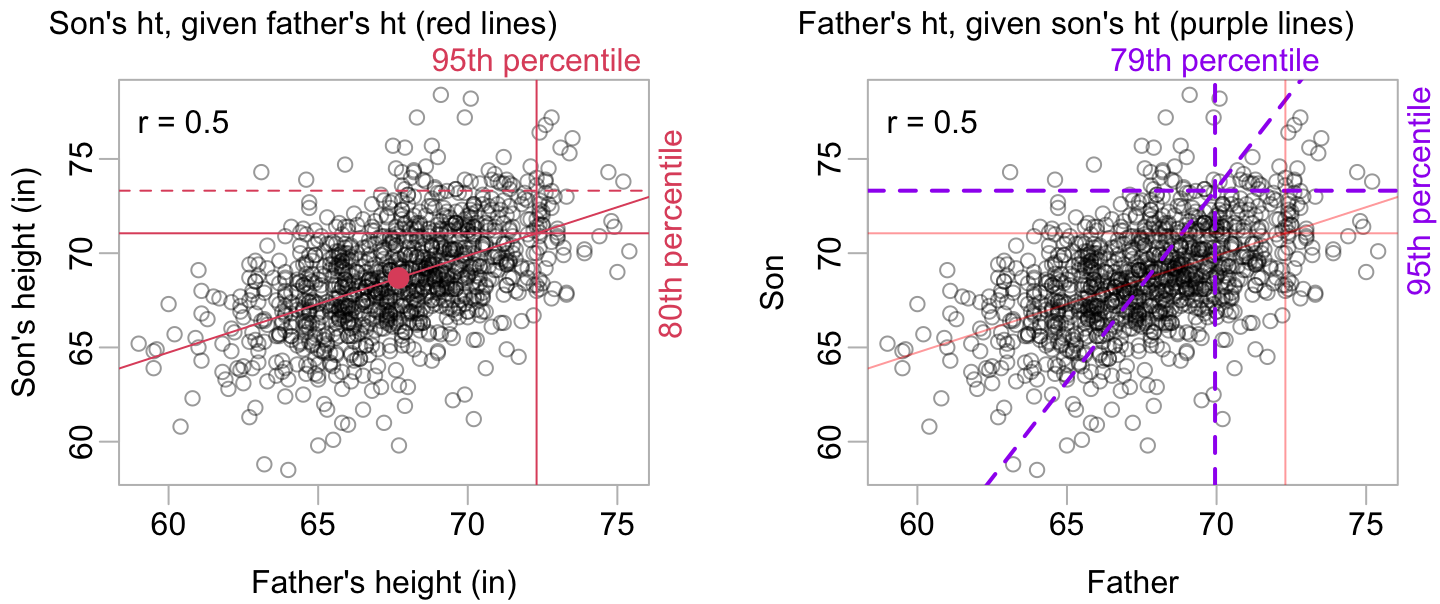
\includegraphics[width=1\linewidth]{08-regress_files/figure-latex/pearson-1} 

}

\caption{Tall fathers are likely to have tall sons, but shorter than themselves. 
Tall sons are likely to have tall fathers, but shorter than themselves.}\label{fig:pearson}
\end{figure}

Consider a father whose height is 72 inches, which is the 95th percentile of heights for fathers. What is a best guess for the height of a son? One can read the predicted value off from the graph (the solid horizontal line in Panel A). Or use the regression equation. Or, reason thus:

\begin{itemize}
\tightlist
\item
  If the correlation between father's height and son's height were 0, the best guess would be the mean for son's, i.e., 68.7 inches
\item
  If the correlation were 1, the son's height would be the 95th percentile of heights for sons, i.e., 73.3 inches.
\item
  But, as the correlation is 0.5, the expected height is 68.7 + 0.5\(\times\)(73.3-68.7) = 71.0 inches, i.e., start at the mean and move 0.5 of the distance up to the 95th percentile.
\end{itemize}

Now consider a son whose height is 73.3 inches (the 95th percentile for sons). The argument now goes:

\begin{itemize}
\tightlist
\item
  The best estimate of the father's~height is 67.7 + 0.5\(\times\)(73.3-67.7)=2.8 inches, i.e., start at the mean for fathers and move 0.5 of the distance up to the 95th percentile.
\end{itemize}

Galton's 1886 data, which predates Pearson's data, shows a 0.46 correlation between child height and the average of the parent height.

\section{NBA player points --- correlations decline over time}\label{nba-player-points-correlations-decline-over-time}

In Figure \ref{fig:NBA}, Panel A shows total points for 2016-2017 versus 1 year earlier, for players who competed in both seasons. The correlation is 0.83. Panel B is for 2016-2017 versus 5 years earlier, with the correlation now reducing to 0.41.

\begin{figure}[H]

{\centering 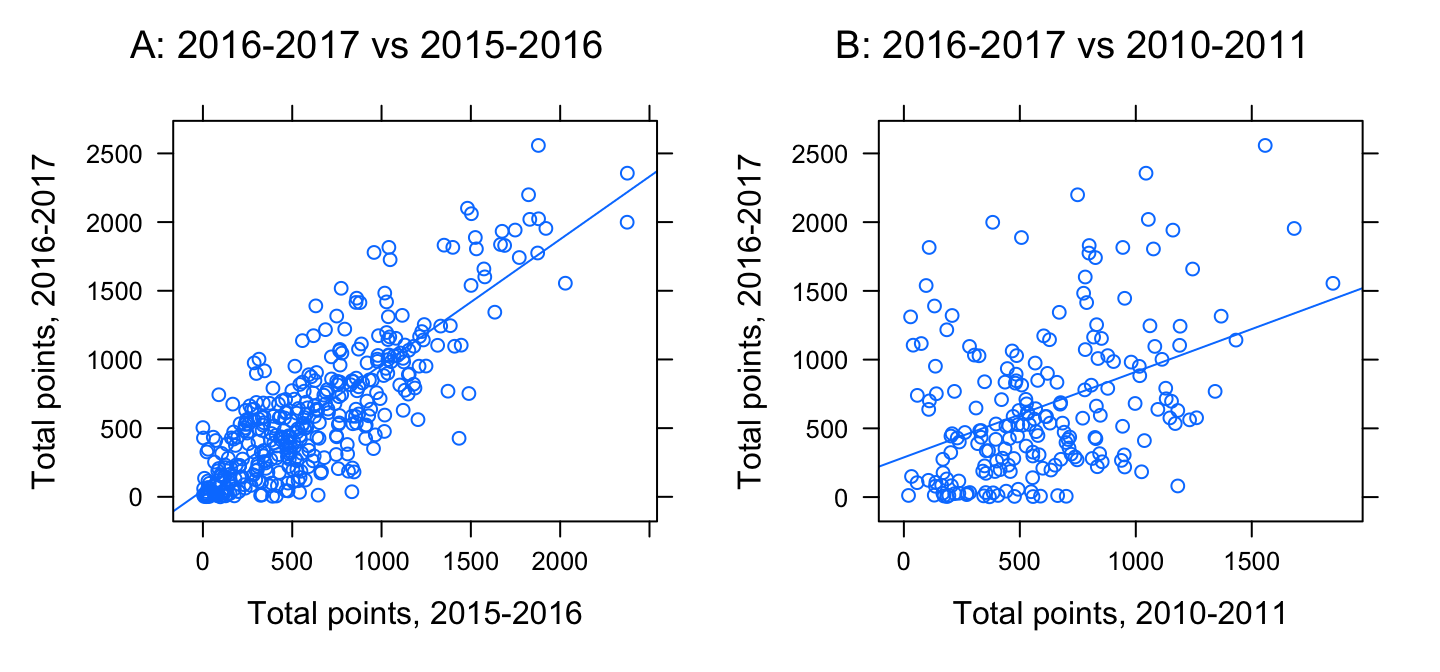
\includegraphics[width=1\linewidth]{08-regress_files/figure-latex/NBA-1} 

}

\caption{As time progresses, correlation decreases, and regression to the mean increases.  For Panel A, the correlation is 0.83, while in Panel B it is 0.41.}\label{fig:NBA}
\end{figure}

The scatter of points increases as values increase, on both axes. Calculations of the type given in the previous section, based on the usual correlation measure, while giving more approximate results, are adequate for present purposes.

\section{Secrist's ``The Triumph of Mediocrity in Business''}\label{secrists-the-triumph-of-mediocrity-in-business}

Horace Secrist's 1933 book The Triumph of Mediocrity in Business'' was based on annual data for 1920 to 1930. Secrist took 73 different industries, in each case examined the ratios

\begin{quote}
Profits:sales; Profits:assets; Expenses:sales; Expenses:assets
\end{quote}

For each industry in 1920: he then split firms into 4 quartiles: top 25\%, 2nd highest 25\%, 2nd lowest 25\%, lowest 25\%.

\begin{itemize}
\tightlist
\item
  Took average for each statistic, for each quartile, for each year.
\item
  Surprise, surprise, the best went, on average, down \ldots{}
\end{itemize}

\begin{quote}
Complete freedom to enter trade and the continuance of competition mean the perpetuation of mediocrity. \ldots{} neither superiority or inferiority will tend to persist. Rather, mediocrity tends to become the rule. (\citeproc{ref-secrist1933triumph}{Secrist 1933})
\end{quote}

\begin{figure}[H]

{\centering 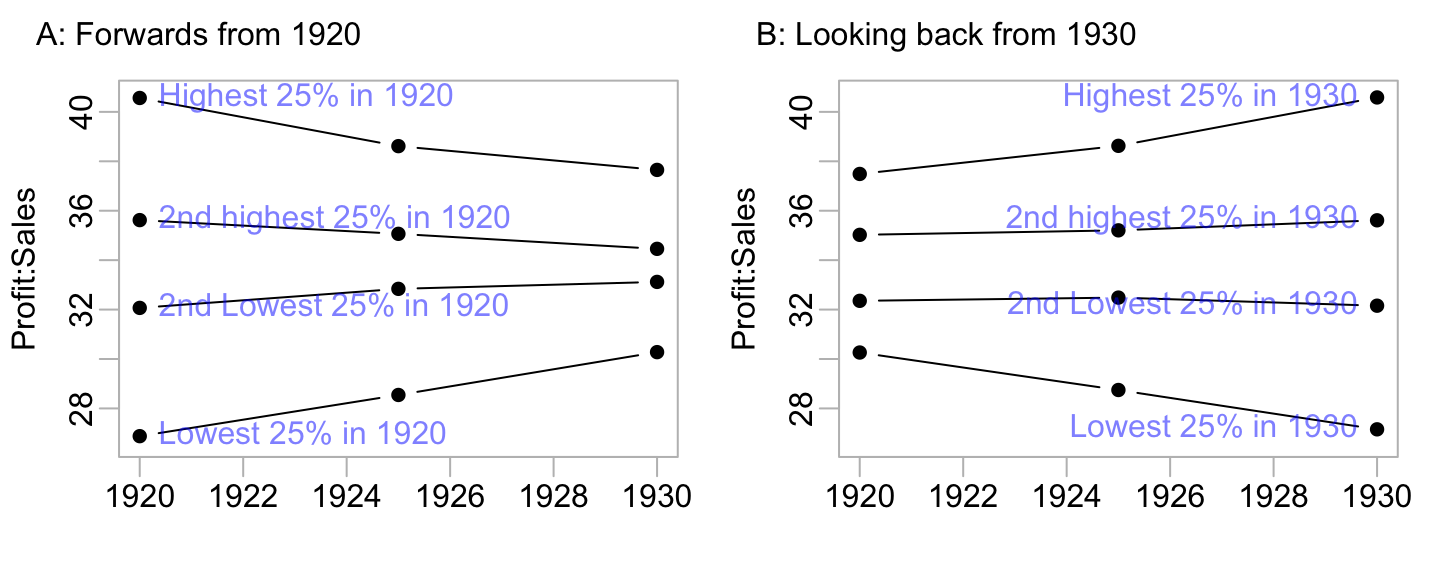
\includegraphics[width=1.05\linewidth]{08-regress_files/figure-latex/sim-1} 

}

\caption{Secrist's data showed a correlation of 0.5 between
time intervals five years apart.  Panel A uses shows means of simulations,
starting with the four performance quartiles in 1920 and looking ahead.
Panel B starts with the equivalent quartiles in 1930, and looks back.}\label{fig:sim}
\end{figure}

Secrist was seeing regression to the mean. Figure \ref{fig:sim} makes the point that if one takes the four quartiles in 1930 and looks back to 1920, in each case there is a regression back to the mean. Given a correlation of 0.7 between time intervals five years apart, The absolute difference from the mean moves from 8 to 0.7\(\times\) 8 (= 5.6) to 0.7\(\times\) 5.6 (= 3.92), whether one moves by two successive five year intervals forward in time, or back in time.

\subsection*{``Do old fallacies ever die?''}\label{do-old-fallacies-ever-die}
\addcontentsline{toc}{subsection}{``Do old fallacies ever die?''}

Smith (\citeproc{ref-smith-sd}{2014}) gives references to work by prominent economists in the past half-century that had quoted Secrist approvingly or repeated his error.

\begin{itemize}
\tightlist
\item
  1980s investment textbook: ``Ultimately, economic forces will force the convergence of the profitability and growth rates of different firms.'' This was backed up with a 1980/1966 Secrist type comparison.
\item
  2000: (Journal article) ``\ldots{} profitability is mean-reverting within as well as across industries. Other firms eventually mimic products and technologies that produce above normal profitability \ldots{}''
\item
  Wainer (\citeproc{ref-wainerRegress}{2000}) cites other examples.
\end{itemize}

\subsection*{Decathlon performances in 2006}\label{decathlon-performances-in-2006}
\addcontentsline{toc}{subsection}{Decathlon performances in 2006}

\begin{figure}[H]

{\centering 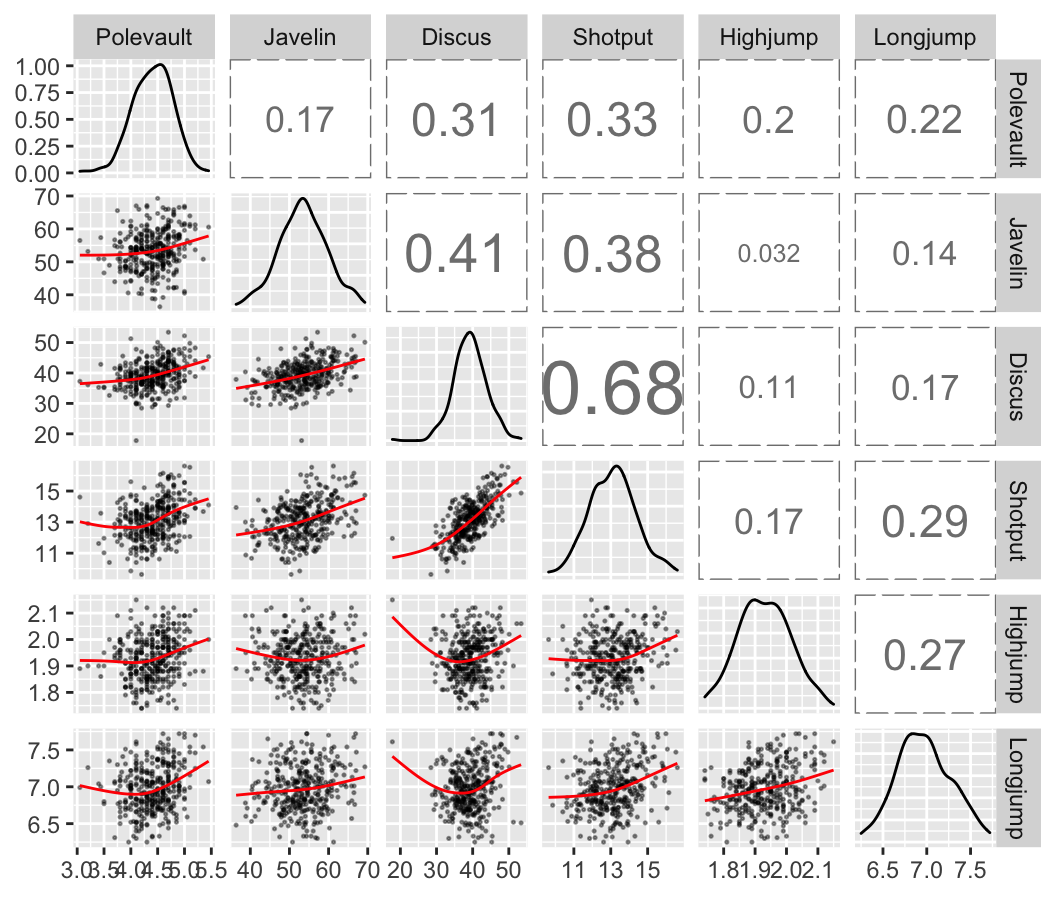
\includegraphics[width=0.68\linewidth]{08-regress_files/figure-latex/selected-1} 

}

\caption{Between event correlations for top performances in six
of the ten decathlon events in 2006.  Points that are plotted,
and correlations, are for times or distances achieved.}\label{fig:selected}
\end{figure}

Figure \ref{fig:selected} shows between event correlations for top performances (6800 points and over) for six events in the 2006 decathlon.\footnote{The dataset \texttt{Decathlon} in the R package \texttt{GDAdata} has data for the 21-year period after new rules were introduced in 1985. See also the Estonian website \url{http://www.decathlon2000.com/}} Note the 0.032 correlation of javelin with high jump. Performance in one of these two sports was not a useful indicator of what to expect in the other.

The correlation between shot put distances and long jump distances is shown as a more informative 0.29. If we find that an athlete has achieved a distance of 14.9 meters in the shot put, which is at the 93\(^{th}\) percentile across athletes as a whole (7\% did better), a best estimate for the long jump can be obtained thus:

\begin{itemize}
\tightlist
\item
  A 14.9 meter put is at the 93\(^{th}\) centile (7\% will do better)
\item
  The long jump mean is 6.97, with the 93\% mark = 7.47

  \begin{itemize}
  \tightlist
  \item
    The difference from the mean is 7.47-6.97 = 0.5
  \end{itemize}
\item
  The estimate for the long jump is then 6.97+0.29 \(\times\) 0.5 = 7.12
\end{itemize}

\section{Moderating predictive assessments}\label{moderating-predictive-assessments}

\subsection*{Moderating sales estimates}\label{moderating-sales-estimates}
\addcontentsline{toc}{subsection}{Moderating sales estimates}

You are the sales forecaster for a department store chain. All stores are similar in size and merchandise offered, but random factors affect sales in any year. Overall sales are expected to increase by 10\% from 2020 to 2021. Sales in 2020, with the expected total and mean for 2021 are, in millions of dollars:

\begin{longtable}[]{@{}lll@{}}
\toprule\noalign{}
Store & 2020 & 2021 \\
\midrule\noalign{}
\endhead
\bottomrule\noalign{}
\endlastfoot
1 & 10 & --- \\
2 & 23 & --- \\
3 & 18 & --- \\
4 & 29 & --- \\
TOTAL & 80 t each of the & \\
\end{longtable}

stores in 2021. The mean sales amount in 2021 is predicted to be 22,000,000 dollars? With a correlation of 0.4, the predicted sales for the individual stores are obtained thus:

\begin{longtable}[]{@{}
  >{\raggedright\arraybackslash}p{(\columnwidth - 8\tabcolsep) * \real{0.1045}}
  >{\raggedright\arraybackslash}p{(\columnwidth - 8\tabcolsep) * \real{0.0896}}
  >{\raggedright\arraybackslash}p{(\columnwidth - 8\tabcolsep) * \real{0.1940}}
  >{\raggedright\arraybackslash}p{(\columnwidth - 8\tabcolsep) * \real{0.3582}}
  >{\raggedright\arraybackslash}p{(\columnwidth - 8\tabcolsep) * \real{0.2537}}@{}}
\toprule\noalign{}
\begin{minipage}[b]{\linewidth}\raggedright
Store
\end{minipage} & \begin{minipage}[b]{\linewidth}\raggedright
2020
\end{minipage} & \begin{minipage}[b]{\linewidth}\raggedright
Subtract 20
\end{minipage} & \begin{minipage}[b]{\linewidth}\raggedright
Xply by 0.4, add to 22
\end{minipage} & \begin{minipage}[b]{\linewidth}\raggedright
Predicted sales
\end{minipage} \\
\midrule\noalign{}
\endhead
\bottomrule\noalign{}
\endlastfoot
1 & 10 & -10 & 22-4 & 18 \\
2 & 23 & +3 & 22+1.2 & 23.2 \\
3 & 18 & -2 & 22-0.8 & 21.2 \\
4 & 29 & +9 & 29+3.6 & 32.6 \\
MEAN & 20 & 0 & 22 & 22 \\
\end{longtable}

In the real world of 2020 and 2021, the Covid-19 pandemic makes all such predictions hazardous!

\subsection*{Choosing from job applicants}\label{choosing-from-job-applicants}
\addcontentsline{toc}{subsection}{Choosing from job applicants}

Correlation between presentation \& performance is likely to be lower for the less well-known. In both cases performance is likely, relative to presentation, to move in closer to the mean. For less well-known candidates, the shift towards the mean is likely to~be greater.

\subsection*{Kahneman's comments on regression to the mean}\label{kahnemans-comments-on-regression-to-the-mean}
\addcontentsline{toc}{subsection}{Kahneman's comments on regression to the mean}

\begin{quote}
``Extreme predictions and a willingness to predict rare events from weak evidence are both manifestations of System 1. \ldots{}''
\end{quote}

\begin{quote}
``Regression to the mean is also a problem for System 2. The very idea \ldots{} is alien and difficult to communicate and comprehend. This is a case where System 2 requires special training.''
\end{quote}

\begin{quote}
``We intuitively want to match predictions to the evidence.''
\end{quote}

\begin{quote}
``We will not learn to understand regression from experience.''
\end{quote}

\subsection*{Regression to the mean in verse}\label{regression-to-the-mean-in-verse}
\addcontentsline{toc}{subsection}{Regression to the mean in verse}

\url{https://www.youtube.com/watch?v=sxMllckUWaw}

\section{Time per unit distance for hillraces}\label{time-per-unit-distance-for-hillraces}

Regression coefficients may differ greatly depending on what adjustments are made for other variables. This is important for attaching meaning to a coefficient. For the hillrace data that will now be considered, it is relatively easy to tease out the role of the explanatory variables that have been included in one or alternative versions of the regression equation. Especially where there are three or more explanatory variables, with the manner in which they should enter into the regression equation is unclear, the effect of an individual variable that is of interest can be difficult or impossible to tease out.

The hillrace dataset has record times for 23 Northern Ireland Mountain Running Association hillraces, as given in the 2007 calendar. In the models fitted and graphs shown that follow, the distance measure is \texttt{Dist} (distance converted to kilometers), the climb measure is \texttt{Climb} (vertical distance between lowest and highest point, in meters), and the time measure is \texttt{Time} (in minutes).

How does time per unit distance (\texttt{timePerKm}) vary with distance. We will fit two equations, both with \(y\) = \texttt{timePerKm}.

\begin{figure}[H]

{\centering 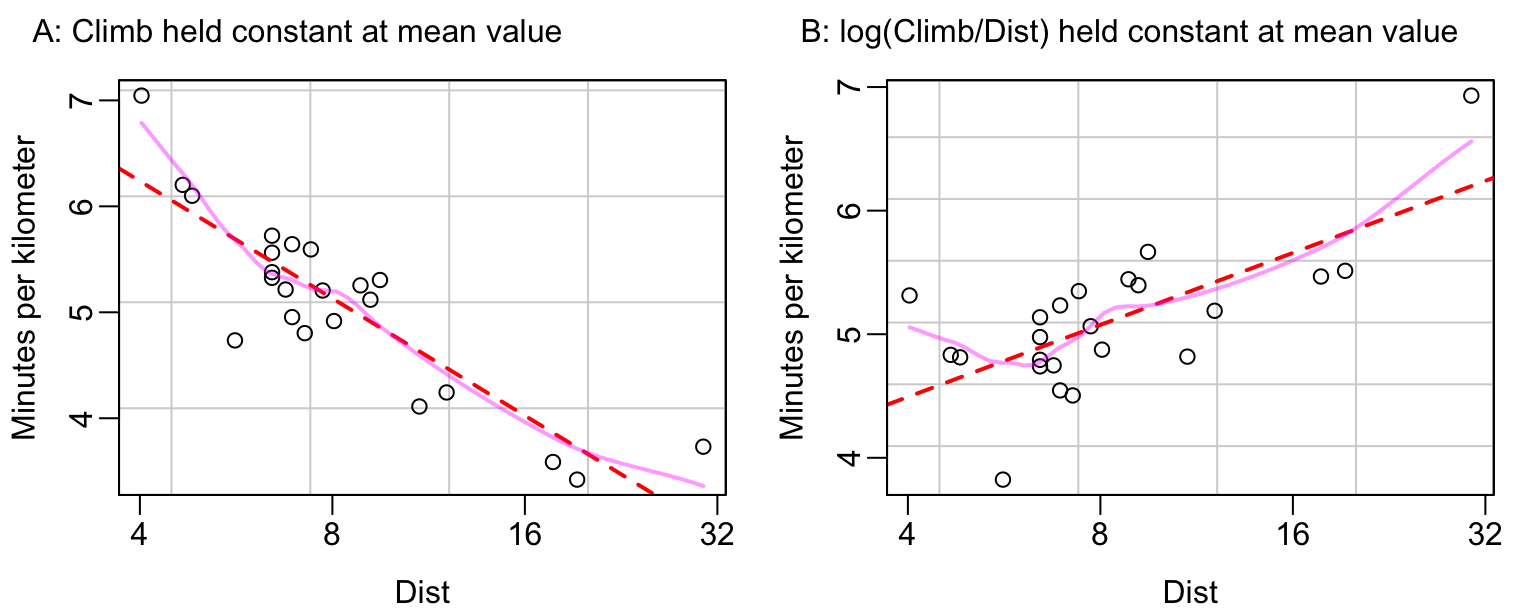
\includegraphics[width=1\linewidth]{08-regress_files/figure-latex/partial-1} 

}

\caption{Variation in time per unit distance with distance.  Panel A
shows the pattern of change when `log(Climb)` is held constant at its 
mean value, while Panel B shows the pattern of change when 
`log(Climb/Dist)` is held constant at its mean value.}\label{fig:partial}
\end{figure}

Figure \ref{fig:partial}A shows the dependence of \texttt{timePerKm} depends on \texttt{log(Dist)}, when \texttt{log(Climb)} is held at its mean value. Use of \texttt{log(Dist)} rather than \texttt{Dist} means that distance on the \(x\)-axis from 2 to 4 (km) is the same as from 4 to 8, or from 8 to 16, or from 16 to 32, i.e., equal distances correspond to equal multiplicative changes. The equation that is plotted is

\begin{quote}
\texttt{timePerKm} = 8.5 -1.6 \(\times\) \texttt{log(Dist)}
\end{quote}

Figure \ref{fig:partial}B shows the dependence of \texttt{timePerKm} depends on \texttt{log(Dist)}, when \texttt{log(Climb/Dist)} is held at its mean value. The equation that is plotted is

\begin{quote}
\texttt{timePerKm} = 3.33 + 0.84 \(\times\) \texttt{log(Dist)}
\end{quote}

In Panel A, time per kilometer decreases quite sharply as distance increases. This happens because the ratio of \texttt{Climb} to \texttt{Dist} decreases if \texttt{Climb} is held constant while \texttt{Dist} increases, i.e., longer distance races involve gentler ascents and descents.

Panel B~shows what happens when \texttt{Climb/Dist} is held constant, i.e., we are comparing races with the same ratio of \texttt{Climb} to \texttt{Dist}. As expected, time per kilometer does then decrease as distance increases.

\section{Model that do not correctly fit the data readily mislead}\label{model-that-do-not-correctly-fit-the-data-readily-mislead}

\subsection*{Are herricanes more dangerous than himmicanes?}\label{are-herricanes-more-dangerous-than-himmicanes}
\addcontentsline{toc}{subsection}{Are herricanes more dangerous than himmicanes?}

\begin{figure}[H]

{\centering 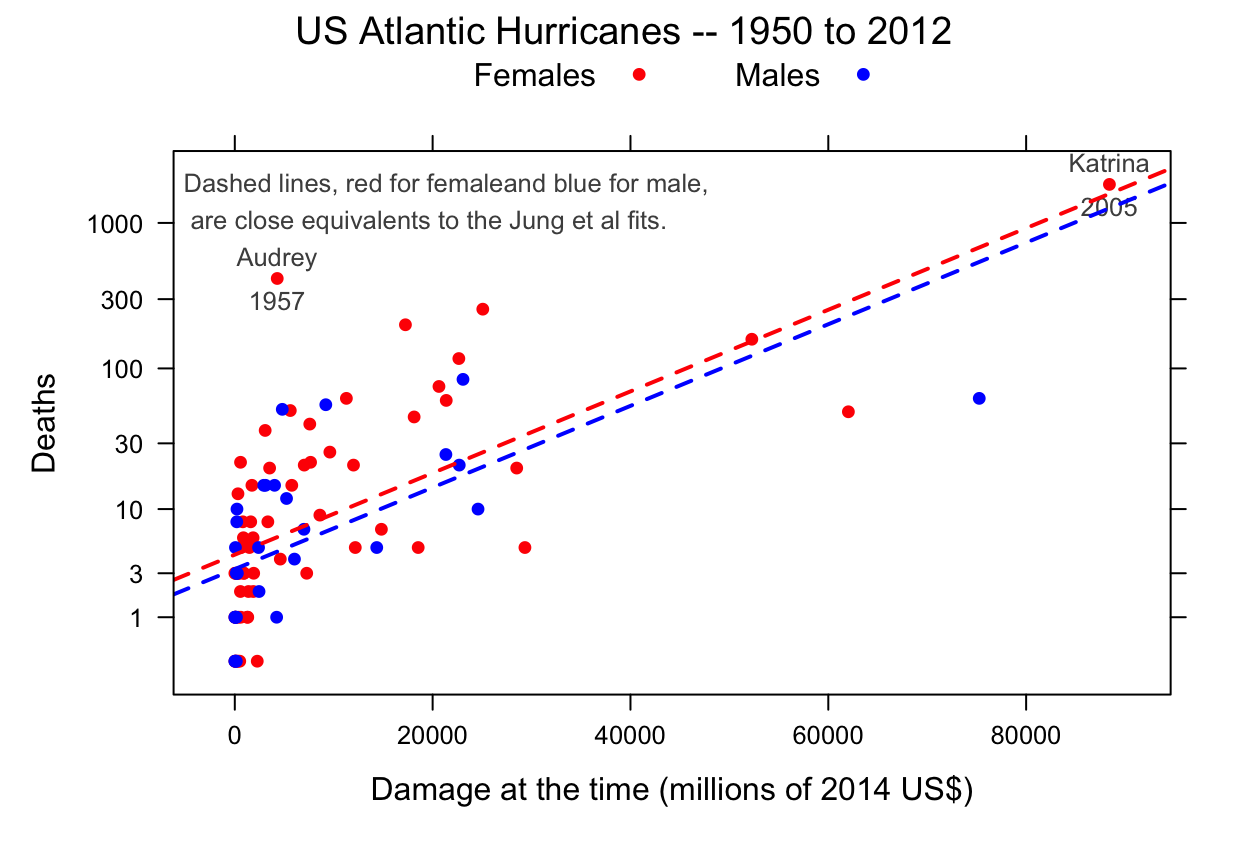
\includegraphics[width=0.8\linewidth]{08-regress_files/figure-latex/hurricanes1-1} 

}

\caption{Deaths versus damage estimate in US dollars. The red (for female) 
and blue (for male) dashed lines are close equivalents of Jung at al's fit
to the data. The $y$-axis uses a scale of equal relative numbers of deaths, 
while the $x$-axis uses a scale of equal dollar damage costs.}\label{fig:hurricanes1}
\end{figure}

The United States National Hurricane Center began formally naming hurricanes in 1950, a task now under control of the World Meteorological Organization. Female names were used for Atlantic hurricanes from 1953 to 1978, with a mix of male and female names used from 1979 onwards.

In a paper titled ``Female hurricanes are deadlier than male hurricanes'', Jung et al. (\citeproc{ref-jung2014female}{2014}) used data for 94 Atlantic hurricanes that made landfall in the United States during 1950-2012 to argue that death rates from those with female names were overall higher than for those with male names. The suggestion was that where names were female, authorities took the risk less seriously. The paper attracted wide interest on the blogosphere, with female hurricanes jokingly called herricanes and males called himmicanes.

\begin{figure}[H]

{\centering 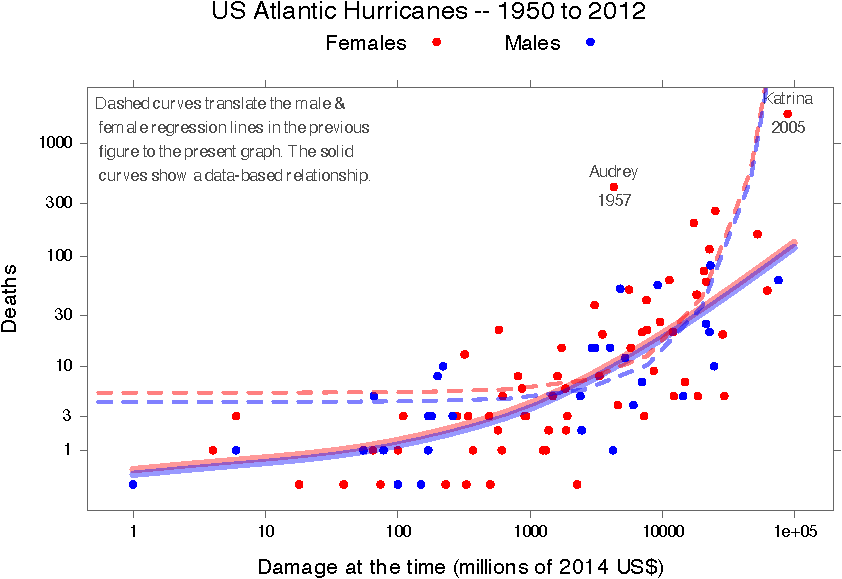
\includegraphics[width=0.8\linewidth]{08-regress_files/figure-latex/hurricanes2-1} 

}

\caption{Deaths versus damage estimate in US dollars, with logarithmic scales
               on both axes. Separate fitted lines for male and female
               hurricanes cannot be distinguished. Jung et al used a 
               logarithmic scale on the vertical axis only, which on
               this graph leads to the dashed curves.}\label{fig:hurricanes2}
\end{figure}

The separate dotted lines in Figure \ref{fig:hurricanes1}, red for female and blue for male, are a close equivalent to the authors' fit to the data. Notice the use of a relative (numbers of deaths) scale on the \(y\)-axis, and a dollar scale on the \(x\)-axis. An unfortunate~consequence of the use of a linear dollar scale on the \(x\)-axis is that the slopes of the lines are strongly influenced by the final four points at the upper~end of the scale. Why did the authors not use, at least as a starting point, the same relative scale on both axes, as in Figure \ref{fig:hurricanes2}?

As well as using a relative scale on the \(x\)-axis, Figure \ref{fig:hurricanes2} uses a methodology that allows the data to determine the form of the response. Deaths do on average increase more at a higher rate than the damage measure, but not at the rate suggested by the dashed curves. There is now no evident difference between the two curves.

Jung et al omitted \texttt{Audrey} (in 1957) and \texttt{Katrina} (in 2005), as outliers. These are included in Figures \ref{fig:hurricanes1} and \ref{fig:hurricanes2}, with the curves fitted using a ``robust'' fitting method that is relatively insensitive to outliers. Other differences between the Jung et al analysis, and the analyses reflected in Figures \ref{fig:hurricanes1} and \ref{fig:hurricanes2} are documented in Note 1 , on p.~\pageref{hurricanes}

\subsection*{Historical speed of light estimates --- is there a pattern?}\label{historical-speed-of-light-estimates-is-there-a-pattern}
\addcontentsline{toc}{subsection}{Historical speed of light estimates --- is there a pattern?}

\begin{figure}[H]

{\centering 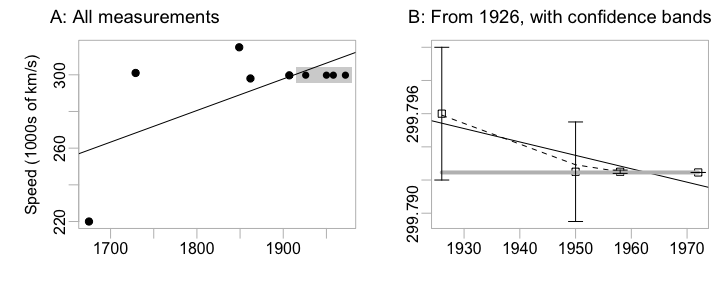
\includegraphics{08-regress_files/figure-latex/plot-c-data-1} 

}

\caption{Successive speed of light estimates.  Panel B 
limits attention to measurements made in 1926 and later. 
The line was fitted with no adjustment for the very
different error estimates.  The dashed curve, which 
incorporates such adjustments, is statistically 
indistinguishable from the thick gray horizontal line.}\label{fig:plot-c-data}
\end{figure}

Creationist Barry Setterfield has argued that a reduction over time in the speed of light has led the passage of time to slow down, relative to the remote past, so that the universe is thousands rather than billions of years old. His arguments rely on making various adjustments to figures obtained historically, selecting what he regarded as the most reliable data, and then fitting a curve.

Setterfield tells a story that, while a little different from that of the line in Panel A of Figure \ref{fig:plot-c-data}, makes equally little sense. The right panel is limited to the points from 1926 and on, marked off with the gray background on the left panel.\footnote{Data are from \url{https://en.wikipedia.org/wiki/Speed_of_light}}

For the measurements from 1862 onward, estimates of accuracy are available. Until 1950, each new estimate lay outside the bounds for the previous estimate, indicating that these were underestimates. Even if one were to accept Setterfield's manipulation of the data, it makes no sense at all to fit either lines such as are shown, or curves, to data values which have such very different accuracies.

Even if one were to accept Setterfield's manipulation of the data, it makes no sense at all to fit either lines such as are shown, or curves, to data values which have such very different accuracies as those shown in the graphs. For the measurements from 1862 onwards, estimates of accuracy are available. Until 1950, each new estimate lay outside the bounds for the previous estimate, indicating that these were underestimates.

\subsection{Global mean temperature trends}\label{global-mean-temperature-trends}

Figure \ref{fig:climate} plots global \href{https://iridl.ldeo.columbia.edu/SOURCES/.NASA/.GISS/.GISSTEMP/.Global/.LOTI/}{air and sea surface temperature anomaly data} against year. Anomalies, in hundredths of a degree centigrade, are differences from the 1951-1980 global average. The grey curve plots the average anomaly up to that point in time.

\begin{figure}[H]

{\centering 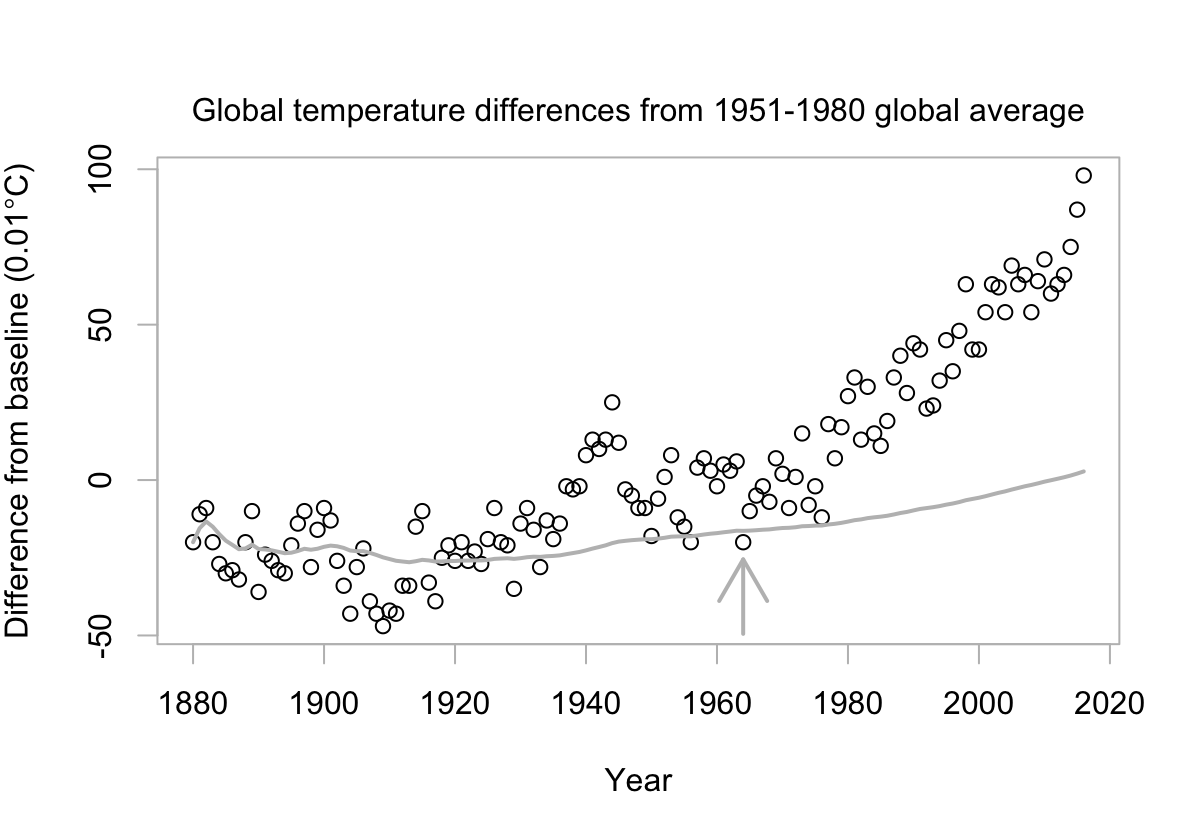
\includegraphics[width=0.8\linewidth]{08-regress_files/figure-latex/climate-1} 

}

\caption{Anomalies (differences) in hundredths of a degree centigrade
from global average temperatures over 1951-1980, plotted against year.
The gray curve shows, for each year, the average anomaly up to that
point in time.  The last year in which this lay below the gray line
was 1962.}\label{fig:climate}
\end{figure}

Observe that 1964 was the last year in which the global temperature fell below the average to that time. For the 52 subsequent years (from 1965 to 2016 inclusive), the global average was above the average up to that date. Under the (false) assumption that global temperature is varying randomly (and therefore independently) about a common mean, the probability of this happening is 2\(^{-40}\) = 9.1 \(\times\) 10\(^{-13}\). A variation of this argument came from a speaker on the Australian ABC Science Show on April 3 2011.

Under any model that accounts for what are now fairly well understood patterns of correlation over time, the probability, while very small, is not that small! Arguments that overstate the case for what is now a well-established pattern of change are unhelpful

It is likewise nonsensical to fit a line to the cherry-picked years 1998-2008, where the trend was relatively flat. Year to year temperatures are correlated.

\chapter{Critiquing scientific claims}\label{critiquing-scientific-claims}

To be credible, scientific claims must be able to survive
informed criticism. The nature of the critique that is
needed will vary, depending on what is in question.
It will vary, at a broader level, depending on whether
what is in question is

\begin{itemize}
\tightlist
\item
  Measurements

  \begin{itemize}
  \tightlist
  \item
    e.g., as in astronomy, distances to other planets,
    stars, and galaxies
  \end{itemize}
\item
  or the results of~an experiment

  \begin{itemize}
  \tightlist
  \item
    e.g., showing that plants grow better when compost is
    added to a nutrient deficient soil
  \end{itemize}
\item
  or a theory, such as Newton's law of gravity or laws of motion.

  \begin{itemize}
  \tightlist
  \item
    A theory is a model that is designed to describe natural
    phenomena. A theory in conceptual, relying on entities
    such as electrons and waves that lie outside of normal
    human experience, where a law is a mathematical description
    of observable phenomena.
  \end{itemize}
\item
  Large parts of science, and scientific applications, rely on
  models that in turn build on scientific theories/laws.

  \begin{itemize}
  \tightlist
  \item
    Epidemiological models have been crucial to informing
    New Zealand's response to the Covid-19 pandemic.
  \end{itemize}
\item
  Climate models are an example of very complex models. These
  rely on

  \begin{itemize}
  \tightlist
  \item
    The basic laws of physics, fluid motion, and chemistry
  \item
    Knowledge of the way that atmosphere, oceans, land
    surface, ice, and solar radiation interact to change
    climate.
  \item
    Computer simulation to build in the effects of areas
    of uncertainty.
  \end{itemize}
\end{itemize}

Measurements and experimental~results must be replicable
--- i.e., another experimenter must be able to repeat the
experiment and obtain the same results. Theories must
be able to~make successful predictions.

In areas where results depend on the sharing of data and
skills between different scientists and groups of~scientists,
the critique that authors provide to the work of their fellow
authors will commonly ensure that what is submitted for peer
review is soundly based.

For experimental studies that are designed to stand on
their own, the past decade has seen the emergence of
concerning evidence that a large amount of published
work is, when put to the test, not replicable. The
steps needed to implement change are well understood.
The slow pace of reform is disappointing.

More generally, uncritical and faulty statistical analyses,
such as have been documented earlier in this book, are a
cause for concern. Too~often, model fitting becomes a ritual,
without the use of standard types of diagnostic checks that
would have demonstrated that the model was faulty.\\
Stark and Saltelli (\citeproc{ref-stark2018cargo}{2018}) comment:

\begin{quote}
The mechanical, ritualistic application of statistics is contributing to a crisis in science. Education, software and peer review have encouraged poor practice--and it is time for statisticians to fight back.
. . .
The problem is one of cargo-cult statistics - the ritualistic miming of
statistics rather than conscientious practice. This has become the norm
in many disciplines, reinforced and abetted by statistical education,
statistical software, and editorial policies.
\end{quote}

It is not just statisticians who should be fighting back, but all
scientists who care about the public credibility of scientific
processes.

\section{What results can be trusted?}\label{what-results-can-be-trusted}

Scientific processes work best when claims made by one scientist
or group of scientists attract widespread interest and critique
from a wider group of scientists who understand the work well
enough to provide informed and incisive criticism. This can be
an effective way to identify claims that have no sound basis.
Examples are the May 2020 Lancet and New England Journal of
Medicine studies, claiming to~be based on observational data,
arguing that use of the drug hydroxychloroquine as a treatment
for Covid-19 was increasing patient deaths.\\
Issues with these papers were quickly identified because they
made claims that bore on an issue of major concern,~and attracted
attention from readers who carefully scrutinized their detailed
statements. They were quickly retracted. How much that has no
sound basis does that attract such attention, and is never
challenged?

Heavy reliance on the sharing of data and skills, and full use of
the benefits that modern technology has to offer, have been vital
to progress in such areas as earthquake science, the study of
viruses and vaccines, modelling of epidemics, and climate science.
This sharing of data and skills, and use of modern technology, also
helps in the critique of what has been published earlier.
Areas where there has not been the same impetus for change are much
more susceptible to the damage that arises from systems for funding
and publishing science that encourage the formal publication of
what would better be treated as preliminary results --- a first
stab at an answer. Publication of experimental results should not
be a once-for-all event, but a staged process that moves from
``this looks promising'' to ``has been independently replicated'',
and to post-publication critique.

Publication does not of itself validate scientific claims,
Rather, as stated in Popper (\citeproc{ref-popper_1963}{1963})

\begin{quote}
Observations or experiments can be accepted as supporting a theory (or a hypothesis, or a scientific assertion) only if these observations or experiments are severe tests of the theory -- or in other words, only if they result from serious attempts to refute the theory.
\end{quote}

The demand that experimental results are shown to be replicable is
central to effective scientific processes. As Fisher (\citeproc{ref-fisher_1937}{1937}) wrote

\begin{quote}
No isolated experiment, however significant in itself, can suffice for the experimental demonstration of any natural phenomenon . . . In order to assert that a natural phenomenon is experimentally demonstrable we need, not an isolated record, but a reliable method of procedure.
\end{quote}

\subsection*{Sources of failure}\label{sources-of-failure}
\addcontentsline{toc}{subsection}{Sources of failure}

Fraud, though uncommon, happens more often than one might hope.
What is disturbing is the small number of scientists with
large numbers of papers that were retracted on account of
fraud. How were they able to get away with publishing so
many papers, usually with fraudulent data, before the
first identification of fraud that led to a checking of all
their work? Ritchie (\citeproc{ref-ritchie2020science}{2020, 67--68})) cites,
as an extreme example, the case of a Japanese anesthesiologist
with 183 retracted papers.

More common are mistakes in data collection, unacknowledged
sources of bias, hype, mistakes or~biases in the handling of
data and/or in data analysis, attaching a much higher
degree of certainty to~statistical evidence than the results
warrant, and selection effects.

What gets published can be strongly affected~by selection
effects. There may be selection of a subset of data where
there appears to be an effect of~interest, choice of the
outcome variable and/or analysis approach that most nearly
gives the result that is wanted, and so on. In analysis of
data from experiments where two treatments are compared,
the common use of the arbitrary \(p \leq 0.05\)
criterion as a cutoff for deciding what will be published
has the inevitable effect of selecting out for publication
one in twenty (or more) results where there was no difference
of consequence.\footnote{Note 2 (p.~\pageref{pval}) in the notes at the end of the book makes relatively technical comments on common misunderstandings that affect the use of \(p\)-values.}

\section{The case of Eysenck and his collaborators}\label{the-case-of-eysenck-and-his-collaborators}

At the time of his death in 1997, Eysenck was the living psychologist
most frequently cited in the peer-reviewed scientific literature.
Much of~his work was controversial in its time, with papers
containing ``questionable data and results so dramatic they beggared
belief'' (\citeproc{ref-o2020famous}{O'Grady 2020}). He relied heavily on what has now been
identified as heavily doctored data that was supplied to him by
German collaborator Grossarth-Maticek. Particularly egregious was
the claim that individuals with an identifiably cancer-prone personality
had a risk of dying from cancer that was as much as 121 times higher
than that of people with a ``healthy'' personality --- one of several
links that the duo~claimed to have found between personality and
mortality. Investigations into~Eysenck's work, including
collaborative work~with Grossarth-Maticek, are ongoing. Fourteen
papers have been retracted, and another 71 have received
``expressions of concern''. A large replication study conducted in
2004 found none of~the claimed links, apart from a modest link between
personality and cardiovascular disease.\footnote{See further Craig, Pelosi, and Tourish (\citeproc{ref-CraigEtAl}{2021}).}

In a book published two years before his death, Eysenck made
comments that provide an intriguing insight into his thinking.

\begin{quote}
Scientists have extremely high motivation to succeed in discovering the truth; their finest and most original discoveries are rejected by the vulgar mediocrities filling the ranks of orthodoxy. .. . . The figures don't quite fit, so why not fudge them a little bit to confound the infidels and unbelievers? Usually the genius is right, of course, and we may in retrospect excuse his childish games, but clearly this cannot be regarded as a licence for non-geniuses to foist their absurd beliefs on us. (\citeproc{ref-eysenck1995genius}{Eysenck 1995, 197})
\end{quote}

Eysenck was alluding to~claims that Newton had manipulated data, and
suggesting that it was excusable for other ``geniuses'' to do the same.

\section{Detection of Covid-19 from chest images}\label{detection-of-covid-19-from-chest-images}

Roberts et al. (\citeproc{ref-roberts2021common}{2021}) identified an astonishing 320 papers and preprints
that appeared between 1 January 2020 to 3 October 2020, and which
describe the use of new machine learning models for the diagnosis of
COVID-19 from chest radiographic (CXR) and chest computed tomography
(CT) images. Quality screening reduced this~number to 62, which were
then examined in more detail. None of the 62 satisfied these more
detailed requirements, designed to check whether the algorithms used
had been shown to~be effective for~use in clinical practice. Among
other deficiencies, 48 did not complete any external validation, and
55 had a high risk of bias with respect to at least one of
participants, predictors, outcomes and analysis. A significant number
of systems were~trained on X-rays from adults with covid-19 and
children without, so~that they were likely to detect whether the
X-ray was from adult or child, rather than whether the person had
Covid-19.

In an account of the results that appeared in New Scientist,
Roberts (\citeproc{ref-roberts2021AIcovid19}{2021}) comments that, relative to persisting to
develop a model that will survive a rigorous
checking process and~might be used in practice, ``it is far easier
to~develop~a model with poor rigour and {[}apparent{]} excellent
performance and publish this.'' This is a damning indictment of
the way that large parts of the research and publication process
currently work. The public good would~be much better served
by a process that encourages researchers to persist until it
has been demonstrated that researchers have a model that meets
standards such as are set out in Roberts (\citeproc{ref-roberts2021common}{2021}).

\section{Laboratory studies --- what do~we find?}\label{sec:lab}

In the past several years, there has been a steady accumulation
of evidence that relates to the claim, in Ioannidis (\citeproc{ref-r19_ioannidis_2005}{2005}),
that ``most published research findings are false''. Ioannidis
has in mind, not published results in general, but primarily
laboratory studies. Papers that have added to the
body of evidence that broadly support claims made in the
Ioannidis paper include:

\begin{itemize}
\tightlist
\item
  Amgen: Reproduced 6 only of 53 `landmark' cancer studies.

  \begin{itemize}
  \tightlist
  \item
    Begley and Ellis (\citeproc{ref-r23_begley_ellis_2012}{2012})
  \item
    Begley (\citeproc{ref-r2_begley_2013}{2013}) notes issues with the studies that failed
  \end{itemize}
\item
  Bayer: Main results from 19 of 65 `seminal' drug studies

  \begin{itemize}
  \tightlist
  \item
    NB, journal impact factor was not a good predictor!
  \item
    Prinz, Schlange, and Asadullah (\citeproc{ref-r9_prinz_schlange_asadullah_2011}{2011})
  \end{itemize}
\item
  fMRI studies: 57 of 134 papers (42\%) had \(\geq\) 1 case lacking
  check on separate test image.
  Another 14\%, unclear \ldots{}

  \begin{itemize}
  \tightlist
  \item
    Kriegeskorte et al. (\citeproc{ref-r8_kriegeskorte_simmons_bellgowan_baker_2009}{2009})
  \end{itemize}
\end{itemize}

Issues that Begley (\citeproc{ref-r2_begley_2013}{2013}) notes are important both across
the pre-clinical studies such as are his concern, and for
clinical studies such as have been used, and are being used,
the check the effectiveness and side effects of Covid-19
vaccines. Begley comments that the flaws many of the
flaws that he identified ``were identified and expunged from
clinical studies decades ago''. They include

\begin{itemize}
\tightlist
\item
  Were experiments blinded?

  \begin{itemize}
  \tightlist
  \item
    Was recording of all results done by another investigator
    who did not know what treatment had been applied?
  \end{itemize}
\item
  Were basic counts, measurements, and tests such as are done
  using Western blotting (used to detect specific proteins in a
  mixture) repeated?
\item
  Were all results presented?

  \begin{itemize}
  \tightlist
  \item
    One concern is that when images are shown (e.g., of Western
    blot gels), images may be cropped in ways that more clearly
    identify the protein than is really the case.
  \end{itemize}
\item
  Were results shown for crucial control experiments?

  \begin{itemize}
  \tightlist
  \item
    Readers should be provided with evidence that there was
    unlikely to be any bias in the comparison of treatment
    with control.
  \end{itemize}
\item
  Were reagents validated?

  \begin{itemize}
  \tightlist
  \item
    Reagents must be shown to be fit for purpose, with results
    shown from analyses that validate their use.
  \end{itemize}
\item
  Were statistical tests appropriate?

  \begin{itemize}
  \tightlist
  \item
    Begley comments on common analysis flaws.
  \end{itemize}
\end{itemize}

Begley comments

\begin{quote}
What is also remarkable is that many of these flaws were
identified and expunged from clinical studies decades ago.
In such studies it is now the gold standard to blind investigators,
include concurrent controls, rigorously apply statistical tests
and analyse all patients --- we cannot exclude patients because
we do not like their outcomes.
\end{quote}

\subsection*{Positive developments in the psychology community}\label{positive-developments-in-the-psychology-community}
\addcontentsline{toc}{subsection}{Positive developments in the psychology community}

The psychological science community is further advanced in
addressing these issues that many other communities, with
The Center for Open Science (COS) taking a strong lead in
studies designed to document the extent of the issues.

Other Center for Open Science (COS) Projects have included

\begin{itemize}
\tightlist
\item
  The Reproducibility: Psychology project. This replicated
  100 studies, from 100 journals in cognitive and social
  psychology.

  \begin{itemize}
  \tightlist
  \item
    In order to keep~the graph simple, Figure
    \ref{fig:effect-size} limits attention to~the
    subset that relate to social psychology.
  \item
    OSC (\citeproc{ref-osc_EstRep2015}{2015})
  \end{itemize}
\item
  Many Labs --- reproduce 13 classical psych studies

  \begin{itemize}
  \tightlist
  \item
    Of 13 studies --- 10: successful, 1: weakly, 2: no!
  \item
    Plots show scatter across the 36 participating teams
  \item
    Klein et al. (\citeproc{ref-r7_klein_others_2014}{2014})
  \end{itemize}
\item
  Cancer Studies --- 50 ``most impactful'' from 2010-2012

  \begin{itemize}
  \tightlist
  \item
    Kaiser (\citeproc{ref-r5_kaiser_2015}{2015})
  \end{itemize}
\item
  Details from other relevant studies are given in the
  recent~book Ritchie (\citeproc{ref-ritchie2020science}{2020}) ``Science fictions: Exposing
  fraud, bias, negligence and hype in science.''
\end{itemize}

In the areas of science to which these studies relate,
it is then clear that published claims that have not
been replicated are as likely as not to be false. As
Begley (\citeproc{ref-r2_begley_2013}{2013}) notes, however, there are clues that
can allow a discerning to make a judgement on the
credibility that should be given to claims that are
made.

Figure \ref{fig:effect-size} compares the effect size
for the replicate with the effect size for the original,
for the 54 social psychology studies included in the
Reproducibility: Psychology project.

\begin{figure}[H]

{\centering 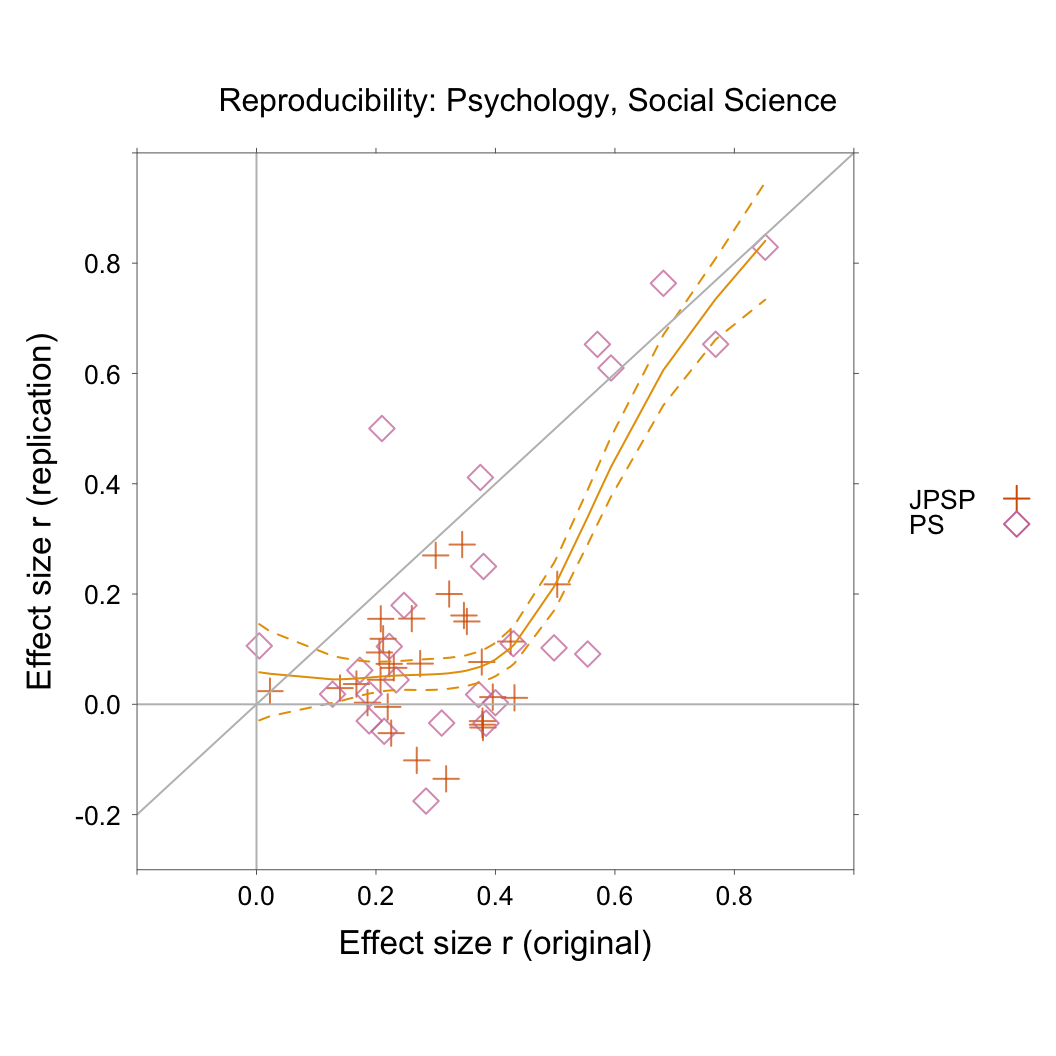
\includegraphics[width=0.6\linewidth]{09-science_files/figure-latex/effect-size-1} 

}

\caption{Psychology reproducibility project. Effect sizes are
compared between the replication and the initial study, for the 
54 social psychology studies included in the Reproducibility:
Psychology project. The journals that are represented are 
Psychological Science (PS), and Journal of Personality and 
Social Psychology (JPSP)}\label{fig:effect-size}
\end{figure}

The effect size is a measure of the average difference found,
divided by an estimate of variability for the individual
results. The effect size is smaller for the replication in 47
out of the 54 studies. A smooth curve, with confidence interval,
has been fitted. It is only for an original effect size
greater than 0.4 that one starts to see a positive correlation
between the effect sizes for the replicate and that for the
original.

\subsection*{Other replication studies}\label{other-replication-studies}
\addcontentsline{toc}{subsection}{Other replication studies}

The critiques have limited relevance to areas where the nature
of the work forces collaboration between scientists with
diverse skills, widely across different research groups.
Where all data and code used in modelling are out in the open
for all to see and evaluate, and research requires co-operation
internationally across multiple areas of expertise, ill-founded
or exaggerated claims are unlikely to survive long. Differences
in the extent to which the nature of the work force co-operation
go a long way to explaining the large variation that is evident
in standards for published work.

Experimental results that have not~been independently
replicated should be treated as provisional, awaiting
confirmation. Replication provides an indispensable
check on all the processes involved. If there are gaps
or inaccuracies in the report and/or supplementary
material that make it impossible to replicate work,
this soon becomes obvious. Another research group,
especially one that has developed expertise in
checking over the work of others, will not usually
repeat the same mistakes.

The peer review process does at least impose some minimal
checks on what is published. In some cases, issues
may be identified subsequent to publication. The case is
at least better than for claims made by those who promote
``alternative medicines'', nowadays often on the internet,
offering ``evidence'' that is anecdotal.

\section{Truths that special interests find inconvenient}\label{truths-that-special-interests-find-inconvenient}

The evidence that human induced greenhouse gas emissions
are driving global warming has for the past two decades
or~more been overwhelming. Fierce criticism of any weakness
in the evidence presented has,~while~delaying effective
action, helped ensure that published work~in this area meets
unusually high standards.

\subsection*{Styles of argument}\label{styles-of-argument}
\addcontentsline{toc}{subsection}{Styles of argument}

The tobacco industry has made extensive use of ``the science is
not settled'' arguments in its efforts to dismiss the evidence
that smoking causes lung cancer. The same PR firms,~and the same
researchers used to support these efforts were later used in the
attempt to undermine climate
science.\footnote{\url{https://www.scientificamerican.com/article/tobacco-and-oil-industries-used-same-researchers-to-sway-public1/}\textgreater{}}
The goal has been to raise doubt, create confusion, and undermine
the science.

In spite of the support that has been available from the fossil
fuel industry for research that is critical of mainstream climate
science research, no substantially different alternative account
has emerged, and no climate change models have emerged that give
results that differ widely from the consensus. Richard Muller's
Berkeley Earth Surface Temperature Study (BEST) is interesting
because Richard Muller had been known for his climate skepticism,
in part based on legitimate scientific concerns. A large part of
the funding came from the right-wing billionaire Charles Koch,
known for funding climate skeptic groups such as the Heartland
Institute.

Muller made headlines when he announced his acceptance of what
climate scientists had been saying for more than 15 years previous:

\begin{quote}
After years of denying global warming, physicist Richard Muller now says ``global warming is real and humans are almost entirely the cause.''\footnote{\url{https://courses.seas.harvard.edu/climate/eli/Courses/global-change-debates/Sources/Hockeystick-global-temperature/more/Richard-Muller/Muller-is-a-believer-Hallelujah.pdf}\textgreater{}}
\end{quote}

The broad sweep of work in climate science is, because it has
survived informed critique, and because of the diversity of
contributing skills and data, unusually secure. Details,
especially as they affect what may happen in individual
countries, are subject to continual revision.

A particular issue is the role of the greenhouse gases, and of
their interactions with water vapour. Their direct effect is
greatly magnified by the consequent warming of the air in which
water vapour is present, allowing it to retain more vapour and trap
more heat). A standard denialist trump card has been to claim the
authority of scientists who have standing in their own areas for
the claim that the contribution of greenhouse gases is small
relative to that of water
vapour.\footnote{See \url{https://west.web.unc.edu/climate-change/} and
  \textless\textgreater{}}
The scientists involved are among a number who have fossil fuel
industry links, and have allowed themselves to be used as
advocates for an industry that sees action on climate change
as a threat.\footnote{\url{https://insideclimatenews.org/news/12032015/leaked-email-reveals-whos-who-list-climate-denialists-merchants-of-doubt-oreskes-fred-singer-marc-morano-steve-milloy}}

\subsection*{Big Pharma --- inconvenient data}\label{big-pharma-inconvenient-data}
\addcontentsline{toc}{subsection}{Big Pharma --- inconvenient data}

Between 1999 and 2019, opioid deaths in the United States increased
by a factor of six, to almost 50,000.
A large contributor has been the increased use of prescription
opioids. Purdue Pharma stands out for its aggressive marketing of
oxycodone, sold under the brand name OxyContin, arguing that
concerns over addiction and other dangers from the drugs were
overblown. In September 2019, Purdue Pharma declared bankruptcy,
facing significant liability in OxyContin and opioid addiction
lawsuits. Details of settlements are still being worked in the
courts.\footnote{ \url{https://topclassactions.com/lawsuit-settlements/open-lawsuit-settlements/opioids/purdue-opioid-addiction-class-action-settlement/}}

Strict regulations govern, in most countries, the approval~of
prescription drugs. Purdue Pharma exploited the much more
limited control over off-label use of approved drugs, i.e.,
use for purposes for which they have not received formal
approval, and for a time stayed under the radar.

Another scandal that demonstrates how drug companies can
sometimes work their way around the approval process
concerns the drug Vioxx, likewise marketed as a
painkiller.(\citeproc{ref-valentine2007timeline}{Valentine and Prakash 2007}) Concerns that the
drug might be increasing the risk of heart attacks began
to~emerge in the months following its approval for use
in May 1999. By November 1, a study set up to investigate
these concerns reported 79 heart attacks out of 4000
among those taking the drug, as opposed to 41 among a
comparator group that was taking naproxen. The drug
continued on the market as the evidence against Vioxx
strengthened further. It was argued, with no evidence
to~back this up, that naproxen likely had a protective
effect. In any case, why allow Vioxx to go to~market
when naproxen was clearly carried less risk.

In September 2004,
when a colon-polyp prevention study showed that Vioxx
increased the risk of heart attack after 18 months,
Merck withdrew the drug. A Lancet paper that was
published later estimated that between 88,000 and
140,000 Americans had heart attacks from taking
Vioxx.\footnote{Jüni et al. (\citeproc{ref-juni2004risk}{2004})} The increased risk continued
long after patients had ceased taking the drug.

\subsection*{What can one trust?}\label{what-can-one-trust}
\addcontentsline{toc}{subsection}{What can one trust?}

One may hope that checks on any new drug will be
stricter than was the case for Vioxx, that lessons
have been learned, that where in future drugs come
up for approval, checks will continue on possible
long-term effects. With fringe and quack medicines,
there are no such checks.

One can take encouragement from the way in which
evidence of the type discussed, that one other drug
is doing more harm than good, has in the cases
discussed finally come to~light. They illustrate
the importance of collecting the relevant data, and
of taking note of what the data have to say.

It has been interesting to follow approval processes
for Covid-19 vaccines. At the time of writing, the
Pfizer, Astrazena and Moderna vaccines have had, in
addition to their testing in clinical trials,
extraordinary levels of testing in clinical practice,
with risks that are small relative to the small risk
that we take ever time we cross a busy road. The
trials, and the use of these vaccines in clinical
practice, have been unusual in the levels of scrutiny
that they have attracted from experts worldwide.

\section{Tricks used to dismiss established results}\label{tricks-used-to-dismiss-established-results}

The headings, and some of commentary, are adapted from an article by
Associate Professor Hassan Vally from La Trobe University,
\href{https://theconversation.com/5-ways-to-spot-if-someone-is-trying-to-mislead-you-when-it-comes-to-science-138814?utm_medium=email&utm_campaign=Latest\%20from\%20The\%20Conversation\%20for\%20March\%209\%202021\%20-\%201883318379&utm_content=Latest\%20from\%20The\%20Conversation\%20for\%20March\%209\%202021\%20-\%201883318379+CID_6009c8d7af2a01f376a88d0491598cfa&utm_source=campaign_monitor&utm_term=5\%20ways\%20to\%20spot\%20if\%20someone\%20is\%20trying\%20to\%20mislead\%20you\%20when\%20it\%20comes\%20to\%20science}{that appeared in \emph{The Conversation} for March 9 2021.}

\begin{enumerate}
\def\labelenumi{\arabic{enumi}.}
\tightlist
\item
  ``The `us versus them' narrative''\\
  The powers that be are trying to deceive us.'' Ask who is
  making the real attempt to deceive --- commercial interest groups,
  peddlers of quack treatments, influence peddlers, . . .
\item
  `I'm not a scientist, but\ldots{}'\\
  Meaning perhaps: ``I'm not a scientist, but that does not stop me
  making an authoritative pronouncement that flies in the face of
  established results.'' Or: ``I know what the science says, but
  I'm keeping an open mind''. Politicians are among the most
  frequent offenders.
\item
  Reference to `the science not being settled'\\
  Much science is of course not settled, and one can then
  expect scientists to openly argue different points of view
  based on available evidence. Or, what has come to be accepted
  wisdom, may turn out to be wrong or in need of substantial
  revision. Challenges to~the accepted wisdom have, however, to be
  carefully argued, and themselves survive informed critique.
\item
  Overly simplistic explanations\\
  Oversimplifications and generalizations are central to many
  anti-science arguments. Science is often messy, complex and full
  of nuance. The truth can be harder to explain, and sometimes
  sound less plausible, than a simple but incorrect explanation.
  Simplistic statistical arguments are common, e.g., fit a
  line to world average temperature data for the cherry-picked years
  1998-2008, ignoring year to year correlation as well as influences
  that operate over longer time periods.
\item
  Cherry-picking\\
  One is not entitled to choose one study over another just because it aligns
  with what you prefer to believe. This is not how science works.\\
  Not all studies are equal; some provide much stronger evidence than others.
  The way that choices are made has to stand up to critical scrutiny.
\end{enumerate}

\chapter{Notes}\label{notes}

\section*{\texorpdfstring{1. The Jung et al. (\citeproc{ref-jung2014female}{2014}) US hurricane data}{1. The Jung et al. (2014) US hurricane data}}\label{hurricanes}
\addcontentsline{toc}{section}{1. The Jung et al. (\citeproc{ref-jung2014female}{2014}) US hurricane data}

Figures \ref{fig:hurricanes1} and \ref{fig:hurricanes2} checked for a difference between the fitted male and female line or curve. Jung et al's approach was, instead, to examine whether numbers of deaths varied with the ``femaleness'' of name, as judged by students in 2014.

As a check on how the popularity of a name for each of females and males may have changed with time, Table \ref{tab:changetab} uses US social security administration data to show numbers for names where the range of variation over 1950 to 2012 in the relative number of females was 0.08 or more.

\begin{table}

\caption{\label{tab:changetab}The minimum and maximum value of the relative proportion
of female names, and the difference, are shown for the eight names
that showed the greatest change over the years 1950 to 2012.}
\centering
\begin{tabular}[t]{l|r|r|r|r|r|r|r|r}
\hline
  & Fran & Charley & Cleo & Sandy & Erin & Inez & Carmen & Bret\\
\hline
Minimum & 0 & 0.00 & 0.39 & 0.68 & 0.84 & 0.86 & 0.88 & 0.00\\
\hline
Maximum & 1 & 0.87 & 0.94 & 0.95 & 0.99 & 1.00 & 0.98 & 0.08\\
\hline
Difference & 1 & 0.87 & 0.55 & 0.28 & 0.15 & 0.14 & 0.10 & 0.08\\
\hline
\end{tabular}
\end{table}

In other cases, relative number of females were always either in the range 0 to 0.07 (i.e., mostly female), or in the range 0.93 to 1 (i.e., mostly female).

Figure \ref{fig:plotchanges} shows how the numbers of each sex changed over time, for the first six of the names in Table \ref{tab:changetab}.

\begin{figure}

{\centering 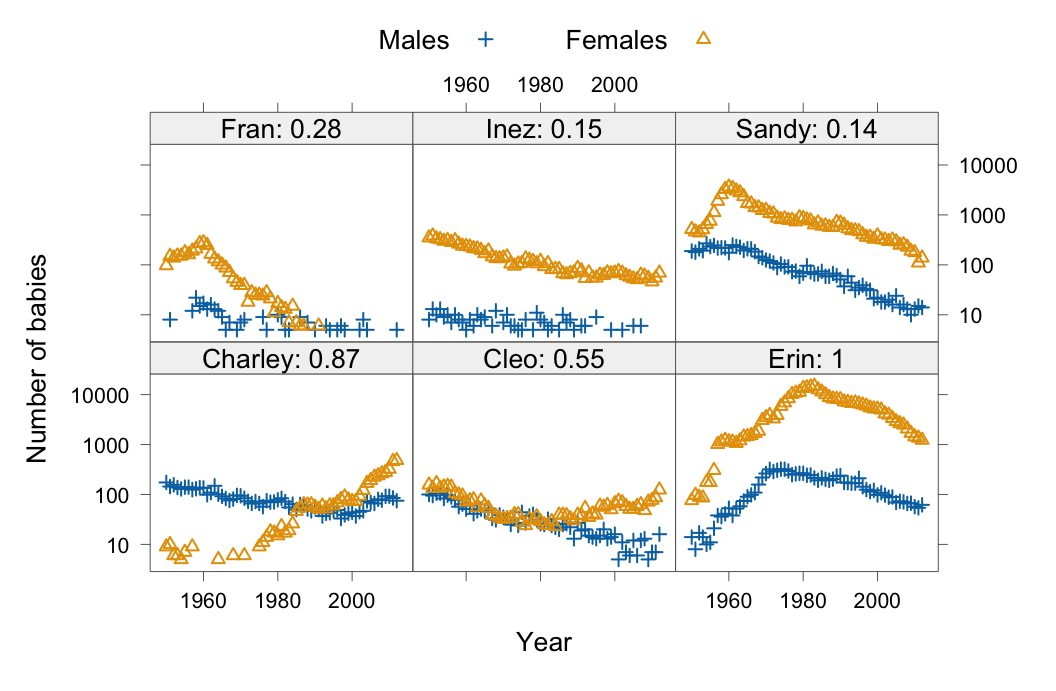
\includegraphics[width=0.9\linewidth]{10-notes_files/figure-latex/plotchanges-1} 

}

\caption{Change in numbers of names given to males and females
over the years 1950 to 2012, for the six names where the 
maximum difference in relative frequency was more than 0.1.
The maximum change is shown against each name.}\label{fig:plotchanges}
\end{figure}

The names where the choices of parents at the time are likely to most different from that for students in 2014 are those where there has been greatest change over time (i.e., especially, Charley, Cleo and Fran).

\enlargethispage{21pt}

Other differences from the analyses on which Figures \ref{fig:hurricanes1} and \ref{fig:hurricanes2} were based are

\begin{itemize}
\tightlist
\item
  As the primary measure of the risk posed by the hurricanes, the authors used a 2013 US\$ estimate of damage, intended for insurance purposes, for a comparable hurricane in 2013. Figure \ref{fig:hurricanes1} uses what is surely the~more relevant measure, namely \texttt{NDAM2014} --- this converts the estimate of damage caused at the time to 2014 US\$.\footnote{Fortuitously, this change makes no difference of consequence to the graph or to the conclusions reached.}
\item
  Jung et al allowed for minor effects from barometric pressure at landfall, and interactions. Again, these do not affect the conclusions reached.
\end{itemize}

\section*{\texorpdfstring{2. \(^*\)What does a \(p\)-value tell the experimenter?}{2. \^{}*What does a p-value tell the experimenter?}}\label{pval}
\addcontentsline{toc}{section}{2. \(^*\)What does a \(p\)-value tell the experimenter?}

\(P\)-values are widely used to indicate whether a difference. What follows introduces technicalities that have been avoided in the preceding chapters.

Consider an experiment that compares a treatment with a control. For example, does taking a drug of interest reduce sleeplessness? The starting point for a \(p\)-value calculation is the NULL hypothesis assumption of no difference in effect between treatment and control. A \(p\)-value measures the probability that a difference in measured effect as large as that observed, or larger would, assuming the NULL hypothesis, occur by chance. The definition says nothing about the \(p\)-value that can be expected if there is a difference. It does not give, as is sometimes thought, the probability that there really is no difference.

Issues for understanding the meaning of a \(p\)-value are:

\begin{itemize}
\tightlist
\item
  Finding \(p \leq 0.05\) is all very well. What one really needs to know is that there is an alternative that is substantially more likely.
\item
  \(p = 0.05\), or close to 0.05, is at the upper end of the range of \(p\)-values that occur with a probability of 0.05. Treating \(p = 0.05\) as an event that occurs with probability 0.05 under the NULL exaggerates the evidence that it provides against the NULL.

  \begin{itemize}
  \tightlist
  \item
    In fact, under the NULL, all values between 0 and 1 are equally likely!
  \end{itemize}
\item
  Prior probabilities matter. If for example the data is from one of a set of drug trials where 99 out of 100 can be expected to show no effect, the 99 out of 100 instances where there is a 1 in 20 change of \(p\) \textless= 0.05 have to be set again 1 out of 100 instances where there is a potential to detect an effect. A \(p\) \textless= 0.05 is more than 99/20 = 4.95 times as likely to come from a drug with no effect as from one that has a real effect.

  \begin{itemize}
  \tightlist
  \item
    What size of effect is, based on whatever is known from past comparable investigations, likely? A reasonable default is to center the distribution on zero, with values that become increasingly less likely as the distance from zero increases. Under plausible assumptions of this general type, it can be shown that with \(p\)=0.05, the prior relative likelihood should be multiplied by, at most, around 2.5.\footnote{See \url{https://statisticsbyjim.com/hypothesis-testing/interpreting-p-values/}}
  \end{itemize}
\end{itemize}

\backmatter

\chapter{Books, videos, and websites}\label{app:more}

\subsection*{Books referred to in the text}\label{books-referred-to-in-the-text}
\addcontentsline{toc}{subsection}{Books referred to in the text}

\begin{itemize}
\tightlist
\item
  Kahneman (\citeproc{ref-kahneman_2013}{2013}) . Thinking, fast and slow.

  \begin{itemize}
  \tightlist
  \item
    \href{https://www.youtube.com/watch?v=PirFrDVRBo4}{Interview with Kahneman}\footnote{\url{https://www.youtube.com/watch?v=PirFrDVRBo4}}
  \item
    \href{https://www.youtube.com/watch?v=uqXVAo7dVRU&t=28s}{A brief animated overview of some key points}\footnote{\url{https://www.youtube.com/watch?v=uqXVAo7dVRU&t=28s}}
  \end{itemize}
\item
  Smith (\citeproc{ref-smith-sd}{2014}) . Standard Deviations: Flawed Assumptions, Tortured Data, and Other Ways to Lie with Statistics

  \begin{itemize}
  \tightlist
  \item
    \href{http://www.garysmithn.com/standard-deviations.html}{Brian Lehrer interview with Smith}\footnote{\url{http://www.garysmithn.com/standard-deviations.html}}
  \end{itemize}
\item
  Ellenberg (\citeproc{ref-ellenberg_2015}{2015}) . How not to be wrong.

  \begin{itemize}
  \tightlist
  \item
    \href{http://www.thelavinagency.com/news/new-videos-jordan-ellenberg-runs-the-numbers}{There are links to several Ellenberg video clips}\footnote{\url{http://www.thelavinagency.com/news/new-videos-jordan-ellenberg-runs-the-numbers}}
  \end{itemize}
\item
  Levitin (\citeproc{ref-levitin_2016}{2016}) . A field guide to lies and statistics.
\item
  Nisbett (\citeproc{ref-nisbett}{2016}) . Tools for smart thinking.
\item
  Cairo (\citeproc{ref-cairo_2013}{2013}) . The functional art: an introduction to information graphics and visualization.
\item
  Ritchie (\citeproc{ref-ritchie2020science}{2020}) . Science fictions: Exposing fraud, bias, negligence and hype in science.
\end{itemize}

\subsection*{Videos}\label{videos}
\addcontentsline{toc}{subsection}{Videos}

\begin{itemize}
\tightlist
\item
  \href{https://www.youtube.com/watch?v=Wy7qpJeozec}{Randomized controlled trials --- animated summary of key issues}\footnote{\url{https://www.youtube.com/watch?v=Wy7qpJeozec}}
\item
  \href{https://www.youtube.com/watch?v=ZDinnCwP3dg}{Yule-Simpson paradox --- animated video}\footnote{\url{https://www.youtube.com/watch?v=ZDinnCwP3dg}}
\end{itemize}

\subsection*{Websites}\label{websites}
\addcontentsline{toc}{subsection}{Websites}

\begin{itemize}
\tightlist
\item
  \href{http://www.bbc.co.uk/editorialguidelines/guidance/reporting-statistics}{BBC links to helpful web resources}\footnote{\url{http://www.bbc.co.uk/editorialguidelines/guidance/reporting-statistics}}
\item
  The \href{https://www.cochrane.org/}{Cochrane Center}\footnote{\url{https://www.cochrane.org/}}
\item
  \href{https://www.hardingcenter.de/en}{Harding Center for Risk Literacy}\footnote{\url{https://www.hardingcenter.de/en}}
\item
  \href{https://wintoncentre.maths.cam.ac.uk/}{Winton Centre for Risk and Evidence Communication}\footnote{\url{https://wintoncentre.maths.cam.ac.uk/}}
\end{itemize}

\chapter*{References}\label{references}
\addcontentsline{toc}{chapter}{References}

\phantomsection\label{refs}
\begin{CSLReferences}{1}{0}
\bibitem[\citeproctext]{ref-anglemyer2014healthcare}
Anglemyer, Andrew, Hacsi T Horvath, and Lisa Bero. 2014. {``Healthcare Outcomes Assessed with Observational Study Designs Compared with Those Assessed in Randomized Trials.''} \emph{Cochrane Database of Systematic Reviews}, no. 4.

\bibitem[\citeproctext]{ref-arkes2012psychological}
Arkes, Hal R, and Wolfgang Gaissmaier. 2012. {``Psychological Research and the Prostate-Cancer Screening Controversy.''} \emph{Psychological Science} 23 (6): 547--53.

\bibitem[\citeproctext]{ref-r2_begley_2013}
Begley, C. G. 2013. {``Reproducibility: Six Red Flags for Suspect Work.''} \emph{Nature} 497 (7450): 433--34. \url{https://doi.org/10.1038/497433a}.

\bibitem[\citeproctext]{ref-r23_begley_ellis_2012}
Begley, C. G., and L. M. Ellis. 2012. {``Drug Development: Raise Standards for Preclinical Cancer Research.''} \emph{Nature} 483 (7391): 531--33. \url{https://doi.org/10.1038/483531a}.

\bibitem[\citeproctext]{ref-boot2008new}
Boot, HM, and JH Maindonald. 2008. {``New Estimates of Age-and Sex-Specific Earnings and the Male--Female Earnings Gap in the British Cotton Industry, 1833--1906 1.''} \emph{The Economic History Review} 61 (2): 380--408.

\bibitem[\citeproctext]{ref-brawley2018prostate}
Brawley, Otis W. 2018. {``Prostate Cancer Screening: And the Pendulum Swings.''} Wiley Online Library.

\bibitem[\citeproctext]{ref-cairo_2013}
Cairo, Alberto. 2013. \emph{The Functional Art: An Introduction to Information Graphics and Vizualisation}. 1st ed. New Riders.

\bibitem[\citeproctext]{ref-chalmers2009avoidable}
Chalmers, Iain, and Paul Glasziou. 2009. {``Avoidable Waste in the Production and Reporting of Research Evidence.''} \emph{The Lancet} 374 (9683): 86--89. https://doi.org/\url{https://doi.org/10.1016/S0140-6736(09)60329-9}.

\bibitem[\citeproctext]{ref-chisholm_2016}
Chisholm, Donna. 2016. {``Birth Control.''} \emph{The NZ Listener, October 8 - 14}, 18--24.

\bibitem[\citeproctext]{ref-cohen1996}
Cohen, P. 1996. {``Pain Discriminates Between the Sexes.''} New Scientist, 2 November 1996.

\bibitem[\citeproctext]{ref-cokely2012measuring}
Cokely, Edward T, Mirta Galesic, Eric Schulz, Saima Ghazal, and Rocio Garcia-Retamero. 2012. {``Measuring Risk Literacy: The Berlin Numeracy Test.''} \emph{Judgment and Decision Making}.

\bibitem[\citeproctext]{ref-coleman2019causality}
Coleman, Thomas. 2019. {``Causality in the Time of Cholera: John {S}now as a Prototype for Causal Inference.''} \emph{Available at SSRN 3262234}.

\bibitem[\citeproctext]{ref-collins_2001}
Collins, Jim. 2001. \emph{Good to Great: Why Some Companies Make the Leap ... And Others Dont}. Random House.

\bibitem[\citeproctext]{ref-CraigEtAl}
Craig, Russell, Anthony Pelosi, and Dennis Tourish. 2021. {``Research Misconduct Complaints and Institutional Logics: The Case of Hans Eysenck and the British Psychological Society.''} \emph{Journal of Health Psychology} 26 (2): 296--311. \url{https://doi.org/10.1177/1359105320963542}.

\bibitem[\citeproctext]{ref-du2015randomized}
Du Toit, George, Graham Roberts, Peter H Sayre, Henry T Bahnson, Suzana Radulovic, Alexandra F Santos, Helen A Brough, et al. 2015. {``Randomized Trial of Peanut Consumption in Infants at Risk for Peanut Allergy.''} \emph{N Engl J Med} 372: 803--13.

\bibitem[\citeproctext]{ref-ellenberg_2015}
Ellenberg, Jordan. 2015. \emph{How Not to Be Wrong}. 1st ed. Penguin Books.

\bibitem[\citeproctext]{ref-erik2007strengthening}
Erik von Elm, MD, Douglas G Altman, Matthias Egger, Stuart J Pocock, Peter C Gøtzsche, and Jan P Vandenbroucke. 2007. {``The Strengthening the Reporting of Observational Studies in Epidemiology (STROBE) Statement: Guidelines for Reporting Observational Studies.''} \emph{Ann Intern Med} 147 (8): 573e7.

\bibitem[\citeproctext]{ref-essermanwisdom}
Esserman, LJ, and WISDOM Study and Athena Investigators. 2017. {``The WISDOM Study: Breaking the Deadlock in the Breast Cancer Screening Debate. NPJ Breast Cancer 3: 34.''} \emph{NPJ Breast Cancer}. \url{https://doi.org/10.1038/s41523-017-0035-5}.

\bibitem[\citeproctext]{ref-eyler1973william}
Eyler, John M. 1973. {``William Farr on the Cholera: The Sanitarian's Disease Theory and the Statistician's Method.''} \emph{Journal of the History of Medicine and Allied Sciences} 28 (2): 79--100.

\bibitem[\citeproctext]{ref-eyler2004changing}
---------. 2004. {``The Changing Assessments of John Snow's and William Farr's Cholera Studies.''} In \emph{A History of Epidemiologic Methods and Concepts}, 129--39. Springer.

\bibitem[\citeproctext]{ref-eysenck1995genius}
Eysenck, Hans Jürgen. 1995. \emph{Genius: The Natural History of Creativity}. 12. Cambridge University Press.

\bibitem[\citeproctext]{ref-farquhar2016letter}
Farquhar, Cynthia, Lesley McCowan, and S Fleming. 2016. {``Letter to the Editor of PloSMedicine.''}

\bibitem[\citeproctext]{ref-fisher_1937}
Fisher, Ronald Aylmer. 1937. \emph{The Design of Experiments}. 2nd ed. Oliver; Boyd.

\bibitem[\citeproctext]{ref-fung2020cancer}
Fung, Jason. 2020. \emph{The Cancer Code: A Revolutionary New Understanding of a Medical Mystery}. Harper Wave.

\bibitem[\citeproctext]{ref-gelman2020regression}
Gelman, Andrew, Jennifer Hill, and Aki Vehtari. 2020. \emph{Regression and Other Stories}. Cambridge University Press.

\bibitem[\citeproctext]{ref-gotzsche2013screening}
Gøtzsche, Peter C, and Karsten Juhl Jørgensen. 2013. {``Screening for Breast Cancer with Mammography.''} \emph{Cochrane Database of Systematic Reviews}, no. 6.

\bibitem[\citeproctext]{ref-harris2016book}
Harris, Ian. 2016. \emph{Surgery, the Ultimate Placebo: A Surgeon Cuts Through the Evidence}. NewSouth.

\bibitem[\citeproctext]{ref-hassall1850memoir}
Hassall, Arthur Hill. 1850. {``Memoir ON THE ORGANIC ANALYSIS OR MICROSCOPIC EXAMINATION OF WATER: Supplied to the Inhabitants of London and the Suburban Districts.''} \emph{The Lancet} 55 (1382): 230--35.

\bibitem[\citeproctext]{ref-herndon2014does}
Herndon, Thomas, Michael Ash, and Robert Pollin. 2014. {``Does High Public Debt Consistently Stifle Economic Growth? A Critique of Reinhart and Rogoff.''} \emph{Cambridge Journal of Economics}. Oxford University Press. \url{http://www.peri.umass.edu/fileadmin/pdf/working_papers/working_papers_301-350/WP322.pdf}.

\bibitem[\citeproctext]{ref-hu2013resolved}
Hu, Frank B. 2013. {``Resolved: There Is Sufficient Scientific Evidence That Decreasing Sugar-Sweetened Beverage Consumption Will Reduce the Prevalence of Obesity and Obesity-Related Diseases.''} \emph{Obesity Reviews} 14 (8): 606--19.

\bibitem[\citeproctext]{ref-r19_ioannidis_2005}
Ioannidis, John P. A. 2005. {``Why Most Published Research Findings Are False.''} \emph{CHANCE} 18 (4): 40--47. \url{https://doi.org/10.1080/09332480.2005.10722754}.

\bibitem[\citeproctext]{ref-jung2014female}
Jung, Kiju, Sharon Shavitt, Madhu Viswanathan, and Joseph M Hilbe. 2014. {``Female Hurricanes Are Deadlier Than Male Hurricanes.''} \emph{Proceedings of the National Academy of Sciences} 111 (24): 8782--87. \url{http://www.pnas.org/cgi/doi/10.1073/pnas.1402786111}.

\bibitem[\citeproctext]{ref-juni2004risk}
Jüni, Peter, Linda Nartey, Stephan Reichenbach, Rebekka Sterchi, Paul A Dieppe, and Matthias Egger. 2004. {``Risk of Cardiovascular Events and Rofecoxib: Cumulative Meta-Analysis.''} \emph{The Lancet} 364 (9450): 2021--29.

\bibitem[\citeproctext]{ref-kahneman_2013}
Kahneman, Daniel. 2013. \emph{Thinking, Fast and Slow}. 1st ed. Farrar, Straus; Giroux.

\bibitem[\citeproctext]{ref-r5_kaiser_2015}
Kaiser, Jocelyn. 2015. {``The Cancer Test.''} \emph{Science} 348 (6242): 1411--13.

\bibitem[\citeproctext]{ref-r7_klein_others_2014}
Klein, Richard A, Kate A Ratliff, Michelangelo Vianello, Reginald B Adams Jr, Štěpán Bahnı́k, Michael J Bernstein, Konrad Bocian, et al. 2014. {``Investigating Variation in Replicability.''} \emph{Social Psychology} 45 (3): 142--52. \url{https://doi.org/10.1027/1864-9335/a000178}.

\bibitem[\citeproctext]{ref-r8_kriegeskorte_simmons_bellgowan_baker_2009}
Kriegeskorte, Nikolaus, W Kyle Simmons, Patrick S F Bellgowan, and Chris I Baker. 2009. {``Circular Analysis in Systems Neuroscience: The Dangers of Double Dipping.''} \emph{Nature Neuroscience} 12 (5): 535--40. \url{https://doi.org/10.1038/nn.2303}.

\bibitem[\citeproctext]{ref-levitin_2015}
Levitin, Daniel J. 2015. \emph{The Organized Mind}. 1st ed. Penguin.

\bibitem[\citeproctext]{ref-levitin_2016}
---------. 2016. \emph{A Field Guide to Lies and Statistics}. 1st ed. Penguin Random House.

\bibitem[\citeproctext]{ref-loberg2015benefits}
Løberg, Magnus, Mette Lise Lousdal, Michael Bretthauer, and Mette Kalager. 2015. {``Benefits and Harms of Mammography Screening.''} \emph{Breast Cancer Research} 17 (1): 1--12.

\bibitem[\citeproctext]{ref-lord1967paradox}
Lord, Frederic M. 1967. {``A Paradox in the Interpretation of Group Comparisons.''} \emph{Psychological Bulletin} 68 (5): 304.

\bibitem[\citeproctext]{ref-martin2018effect}
Martin, Richard M, Jenny L Donovan, Emma L Turner, Chris Metcalfe, Grace J Young, Eleanor I Walsh, J Athene Lane, et al. 2018. {``Effect of a Low-Intensity PSA-Based Screening Intervention on Prostate Cancer Mortality: The CAP Randomized Clinical Trial.''} \emph{JAMA} 319 (9): 883--95.

\bibitem[\citeproctext]{ref-MORAN2022115073}
Moran, Patrick, and John Cullinan. 2022. {``Is Mammography Screening an Effective Public Health Intervention? Evidence from a Natural Experiment.''} \emph{Social Science \& Medicine} 305: 115073. https://doi.org/\url{https://doi.org/10.1016/j.socscimed.2022.115073}.

\bibitem[\citeproctext]{ref-Murphygutjnl-2021-325001}
Murphy, Caitlin C, Piera M Cirillo, Nickilou Y Krigbaum, Amit G Singal, MinJae Lee, Timothy Zaki, Ezra Burstein, and Barbara A Cohn. 2021. {``Maternal Obesity, Pregnancy Weight Gain, and Birth Weight and Risk of Colorectal Cancer.''} \emph{Gut}. \url{https://doi.org/10.1136/gutjnl-2021-325001}.

\bibitem[\citeproctext]{ref-national1975science}
National Science Foundation, DC. National Science Board, Washington. 1975. \emph{Science Indicators, 1974}. Superintendent of Documents.

\bibitem[\citeproctext]{ref-nisbett}
Nisbett, Richard E. 2016. \emph{Mindware. Tools for Smart Thinking.} 1st ed. Penguin Books.

\bibitem[\citeproctext]{ref-o2020famous}
O'Grady, Cathleen. 2020. {``Famous Psychologist Faces Posthumous Reckoning.''} American Association for the Advancement of Science.

\bibitem[\citeproctext]{ref-oneil_2016}
O'Neil, Cathy. 2016. \emph{Weapons of Math Destruction}. 1st ed. Crown.

\bibitem[\citeproctext]{ref-osc_EstRep2015}
OSC. 2015. {``Estimating the Reproducibility of Psychological Science.''} \emph{Science} 349 (6251): aac4716--16. \url{https://doi.org/10.1126/science.aac4716}.

\bibitem[\citeproctext]{ref-pashayan2020personalized}
Pashayan, Nora, Antonis C Antoniou, Urska Ivanus, Laura J Esserman, Douglas F Easton, David French, Gaby Sroczynski, et al. 2020. {``Personalized Early Detection and Prevention of Breast Cancer: ENVISION Consensus Statement.''} \emph{Nature Reviews Clinical Oncology} 17 (11): 687--705.

\bibitem[\citeproctext]{ref-pearl2018book}
Pearl, Judea, and Dana Mackenzie. 2018. \emph{The Book of Why: The New Science of Cause and Effect}. Basic Books.

\bibitem[\citeproctext]{ref-pearson1903laws}
Pearson, Karl, and Alice Lee. 1903. {``On the Laws of Inheritance in Man: I. Inheritance of Physical Characters.''} \emph{Biometrika} 2 (4): 357--462.

\bibitem[\citeproctext]{ref-popper_1963}
Popper, Karl Raimund. 1963. {``Science: Problems, Aims, Responsibilities.''} \emph{Federation of American Societies for Experimental Biology} 22: 961--72.

\bibitem[\citeproctext]{ref-r9_prinz_schlange_asadullah_2011}
Prinz, Florian, Thomas Schlange, and Khusru Asadullah. 2011. {``Believe It or Not: How Much Can We Rely on Published Data on Potential Drug Targets?''} \emph{Nature Reviews Drug Discovery} 10 (9): 712--12. \url{https://doi.org/10.1038/nrd3439-c1}.

\bibitem[\citeproctext]{ref-raichand2017conclusions}
Raichand, Smriti, Adam G Dunn, Mei-Sing Ong, Florence T Bourgeois, Enrico Coiera, and Kenneth D Mandl. 2017. {``Conclusions in Systematic Reviews of Mammography for Breast Cancer Screening and Associations with Review Design and Author Characteristics.''} \emph{Systematic Reviews} 6 (1): 1--8. \url{https://www.ncbi.nlm.nih.gov/pubmed/28532422}.

\bibitem[\citeproctext]{ref-reinhart2010growth}
Reinhart, Carmen M, and Kenneth S Rogoff. 2010. {``Growth in a Time of Debt.''} \emph{American Economic Review} 100 (2): 573--78.

\bibitem[\citeproctext]{ref-ritchie2020science}
Ritchie, Stuart. 2020. \emph{Science Fictions: Exposing Fraud, Bias, Negligence and Hype in Science}. Random House.

\bibitem[\citeproctext]{ref-roberts2021AIcovid19}
Roberts, Michael. 2021. {``Artificial Intelligence Has Been of Little Use for Diagnosing Covid-19.''} New Scientist, 22 May 2021.

\bibitem[\citeproctext]{ref-roberts2021common}
Roberts, Michael, Derek Driggs, Matthew Thorpe, Julian Gilbey, Michael Yeung, Stephan Ursprung, Angelica I Aviles-Rivero, et al. 2021. {``Common Pitfalls and Recommendations for Using Machine Learning to Detect and Prognosticate for COVID-19 Using Chest Radiographs and CT Scans.''} \emph{Nature Machine Intelligence}, no. 3335: 199--217.

\bibitem[\citeproctext]{ref-RosBook}
Rosenbaum, P R. 2002. \emph{Observational Studies}. 2nd ed. Springer.

\bibitem[\citeproctext]{ref-Schulzc332}
Schulz, Kenneth F, Douglas G Altman, and David Moher. 2010. {``CONSORT 2010 Statement: Updated Guidelines for Reporting Parallel Group Randomised Trials.''} \emph{BMJ} 340. \url{https://doi.org/10.1136/bmj.c332}.

\bibitem[\citeproctext]{ref-secrist1933triumph}
Secrist, H. 1933. \emph{The Triumph of Mediocrity in Business}. Business Studies. Bureau of Business Research, Northwestern University. \url{https://books.google.co.nz/books?id=n8RAAAAAIAAJ}.

\bibitem[\citeproctext]{ref-seigworth1980bloodletting}
Seigworth, Gilbert R. 1980. {``Bloodletting over the Centuries.''} \emph{New York State Journal of Medicine} 80 (13): 2022--28.

\bibitem[\citeproctext]{ref-simon1992explanation}
Simon, Herbert A. 1992. {``What Is an {`Explanation'} of Behavior?''} \emph{Psychological Science} 3 (3): 150--61.

\bibitem[\citeproctext]{ref-smith-sd}
Smith, G. 2014. \emph{Standard Deviations: Flawed Assumptions, Tortured Data, and Other Ways to Lie with Statistics}. Duckworth Overlook.

\bibitem[\citeproctext]{ref-snow1849mode}
Snow, John. 1855a. {``On the Mode of Communication of Cholera.''} John Churchill.

\bibitem[\citeproctext]{ref-snow1855mode}
---------. 1855b. \emph{On the Mode of Communication of Cholera}. John Churchill.

\bibitem[\citeproctext]{ref-soni2019comparison}
Soni, Payal D, Holly E Hartman, Robert T Dess, Ahmed Abugharib, Steven G Allen, Felix Y Feng, Anthony L Zietman, Reshma Jagsi, Matthew J Schipper, and Daniel E Spratt. 2019. {``Comparison of Population-Based Observational Studies with Randomized Trials in Oncology.''} \emph{Journal of Clinical Oncology} 37 (14): 1209.

\bibitem[\citeproctext]{ref-stark2018cargo}
Stark, Philip B, and Andrea Saltelli. 2018. {``Cargo-Cult Statistics and Scientific Crisis.''} \emph{Significance} 15 (4): 40--43.

\bibitem[\citeproctext]{ref-thaler2015misbehaving}
Thaler, Richard H, and LJ Ganser. 2015. \emph{Misbehaving: The Making of Behavioral Economics}. WW Norton New York.

\bibitem[\citeproctext]{ref-tu2011statistical}
Tu, Yu-Kang, and Mark S Gilthorpe. 2011. \emph{Statistical Thinking in Epidemiology}. CRC Press.

\bibitem[\citeproctext]{ref-tversky1983extensional}
Tversky, Amos, and Daniel Kahneman. 1983. {``Extensional Versus Intuitive Reasoning: The Conjunction Fallacy in Probability Judgment.''} \emph{Psychological Review} 90 (4): 293.

\bibitem[\citeproctext]{ref-us1989guide}
US Preventive Services Task Force. 1989. \emph{Guide to Clinical Preventive Services: Report of the US Preventive Services Task Force}. Diane Publishing Company.

\bibitem[\citeproctext]{ref-valentine2007timeline}
Valentine, Vikki, and Snigdha Prakash. 2007. {``Timeline: The Rise and Fall of Vioxx.''} \emph{NPR (National Public Radio)} 10.

\bibitem[\citeproctext]{ref-wainerRegress}
Wainer, Howard. 2000. {``Visual Revelations.''} \emph{CHANCE} 13 (1): 47--48. \url{https://doi.org/10.1080/09332480.2000.10542192}.

\bibitem[\citeproctext]{ref-waterman1982search}
Waterman, Robert H, and Thomas J Peters. 1982. \emph{In Search of Excellence: Lessons from America's Best-Run Companies}. New York: Harper \& Row.

\bibitem[\citeproctext]{ref-watkins2000conviction}
Watkins, Stephen J. 2000. {``Conviction by Mathematical Error?: Doctors and Lawyers Should Get Probability Theory Right.''} British Medical Journal Publishing Group.

\bibitem[\citeproctext]{ref-watson2020open}
Watson, J, A Adler, A Agweyu, et al. 2020. {``Open Letter to MR Mehra, SS Desai, f Ruschitzka, and AN Patel, Authors of {`Hydroxychloroquine or Chloroquine with or Without a Macrolide for Treatment of COVID-19: A Multinational Registry Analysis'}.''} \emph{Lancet}, 31180--86.

\bibitem[\citeproctext]{ref-wernham_EtAl_2016}
Wernham, Ellie, Jason Gurney, James Stanley, Lis Ellison-Loschmann, and Diana Sarfati. 2016. {``A Comparison of Midwife-Led and Medical-Led Models of Care and Their Relationship to Adverse Fetal and Neonatal Outcomes: A Retrospective Cohort Study in New Zealand.''} \emph{PLOS Medicine} 13 (9): e1002134. \url{https://doi.org/10.1371/journal.pmed.1002134}.

\bibitem[\citeproctext]{ref-young2014improving}
Young, Scott WH. 2014. {``Improving Library User Experience with a/b Testing: Principles and Process.''} \emph{Weave: Journal of Library User Experience} 1 (1).

\end{CSLReferences}

\newpage

\thispagestyle{empty}

\chapter*{About the author}\label{author}
\addcontentsline{toc}{chapter}{About the author}

For the major part of his career, John Maindonald has worked with other
researchers as a quantitative problem solver.
He has held positions at Victoria University of Wellington, in DSIR, in HortResearch Crown Research Institute (now Plant and Food), and at The Australian National University (ANU).
He joined the then newly formed ANU Centre for Bioinformation Science in 2001, formally retiring in 2005.
Between 1983 and 1996, and occasionally after 1996, he reviewed the statistical content of numerous papers that appeared in DSIR (later, Royal Society) journals, notably the New Zealand Journal of Agricultural Research and the New Zealand Journal of Crop and Horticultural Research.

Between 2003 and 2015, he fronted 35 short courses (one week, or less)
across different parts of Australia that demonstrated the use of the open source R data analysis and graphics system for data analysis purposes.
He is the author of a book on Statistical Computation, and the senior author of
the texts

\begin{itemize}
\tightlist
\item
  \emph{Data Analysis and Graphics Using R --- An Example-Based Approach}, Maindonald and Braun, Cambridge University Press 2010.
  This has sold more than 11,000 copies over the three editions.\\
\item
  \emph{A Practical Guide to Data Analysis Using R -- An Example Based Approach},
  Maindonald, Braun, Andrews. Cambridge University Press 2024 (in press).
\end{itemize}

\end{document}
